\section{Intermediate $\AR$s with $3 < \AR < 4.75$}


\begin{figure}
  \centering
  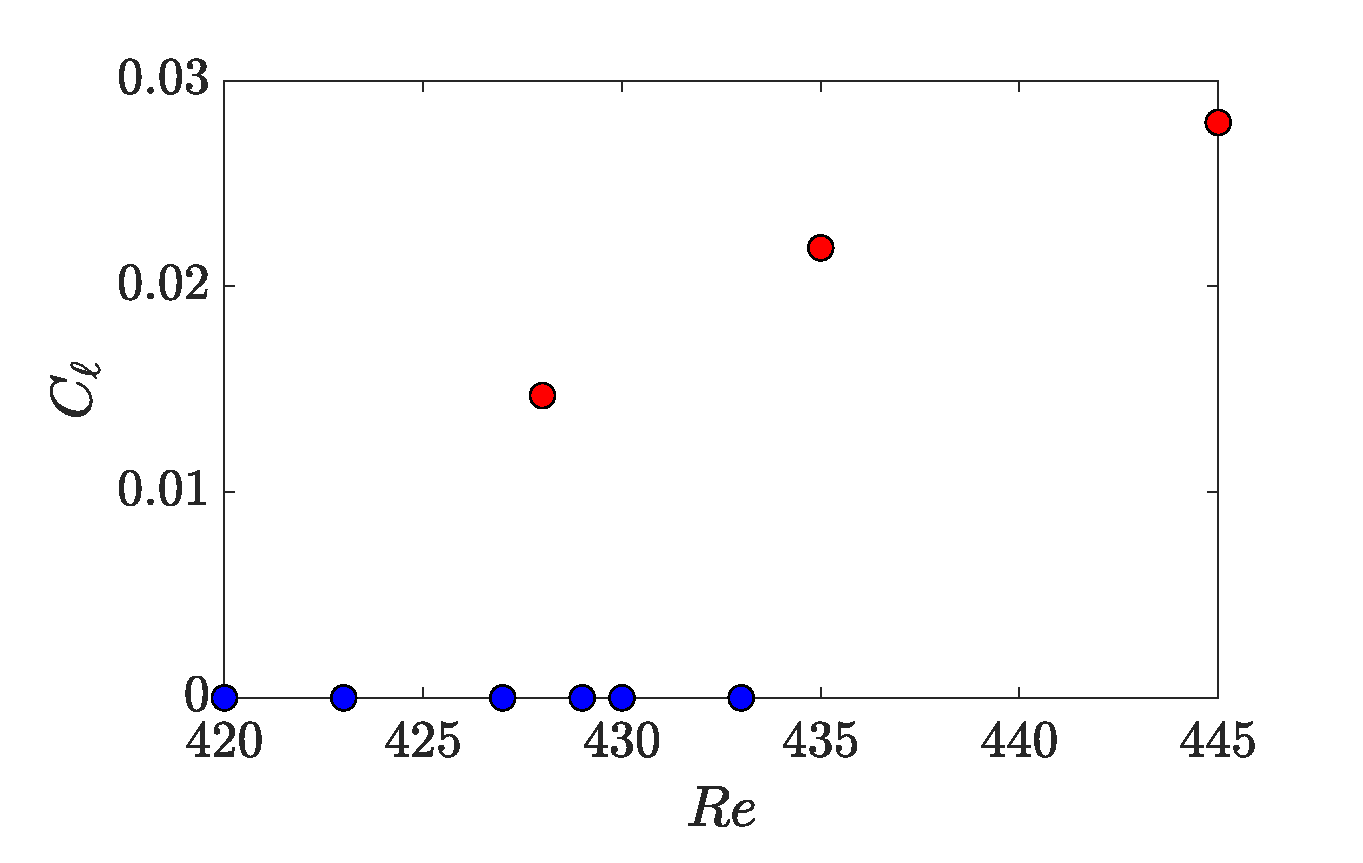
\includegraphics[width=0.49\textwidth]{./fig/AR4_Cl_Re.eps}
  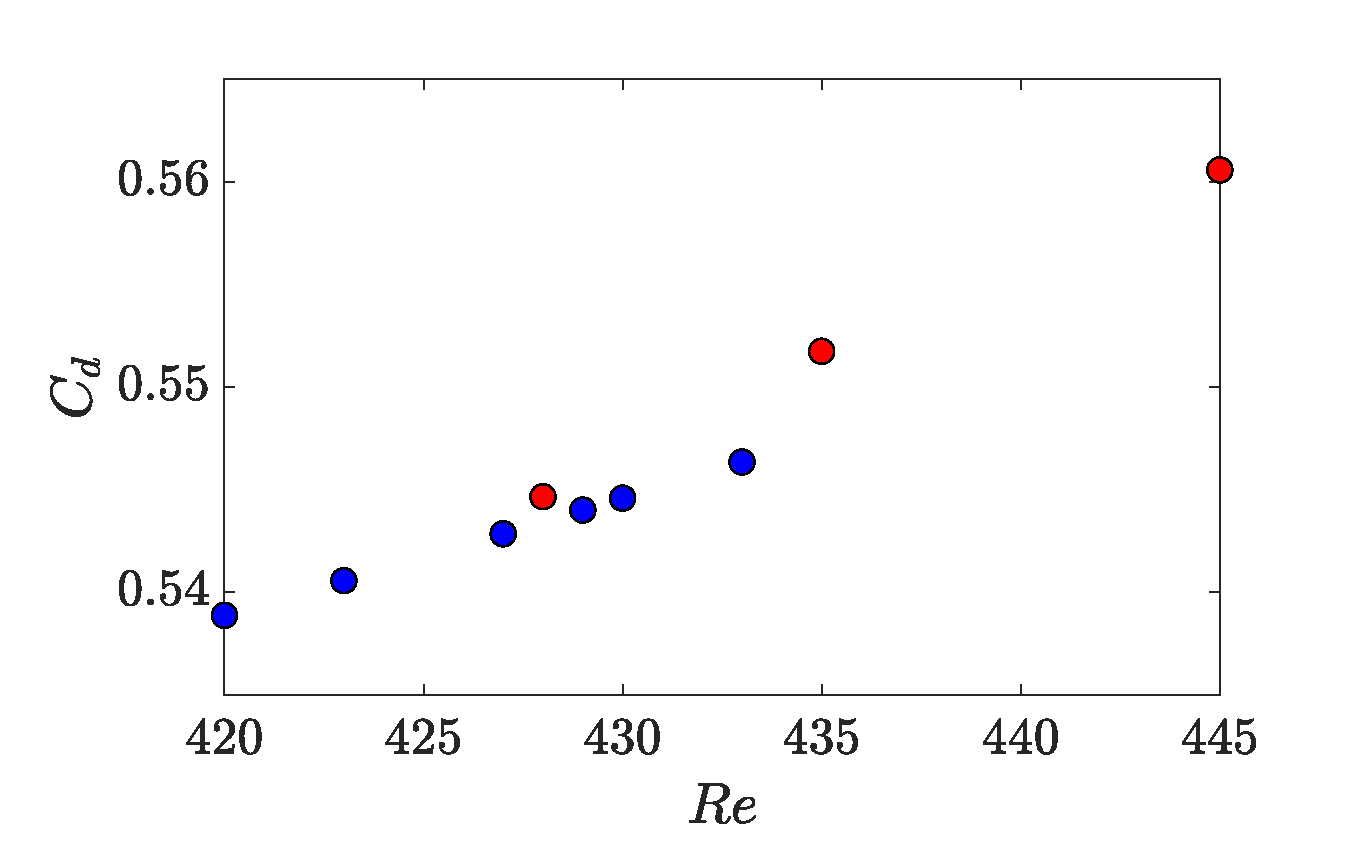
\includegraphics[width=0.49\textwidth]{./fig/AR4_Cd_Re.eps}
  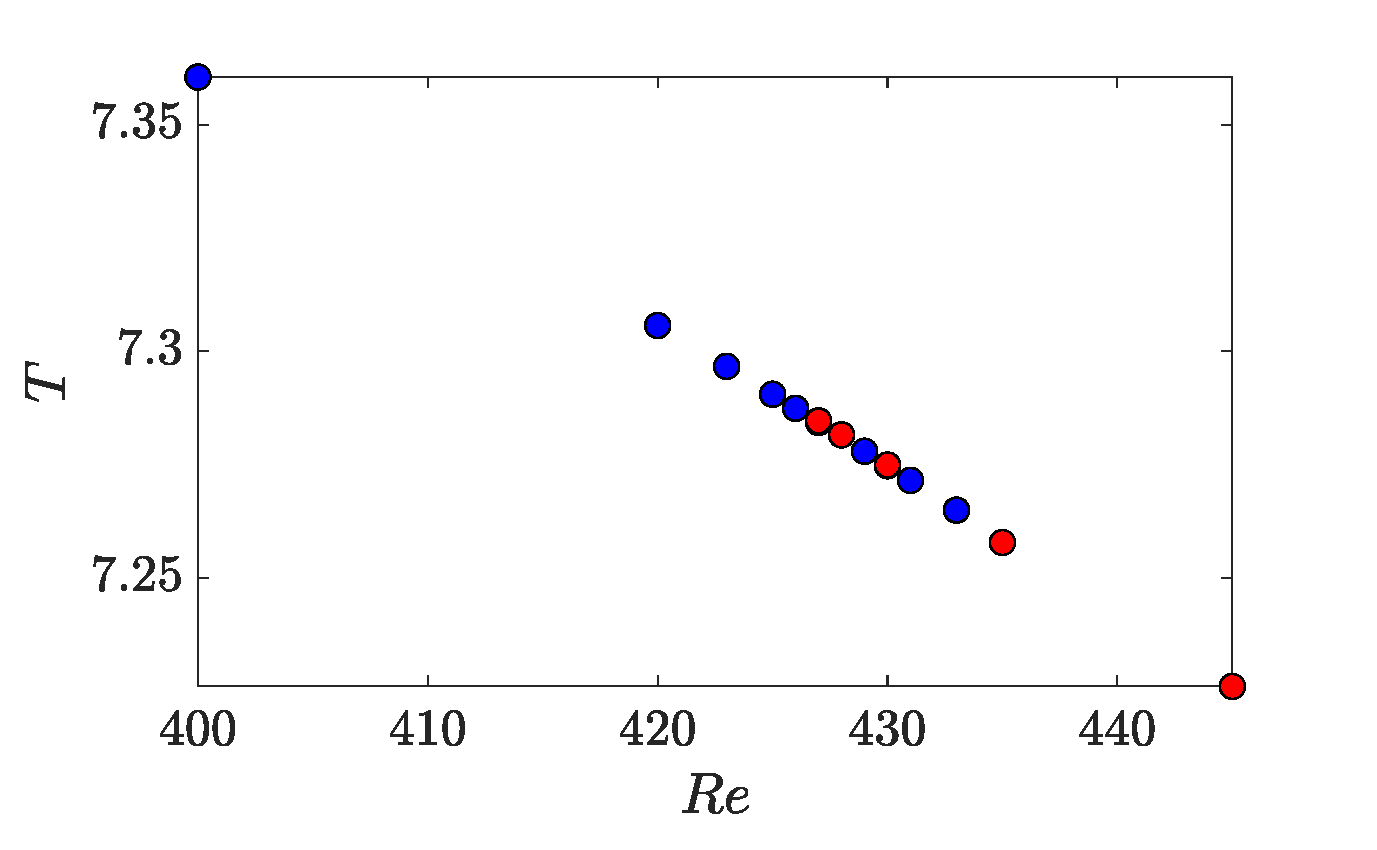
\includegraphics[width=0.49\textwidth]{./fig/AR4_T_Re.eps}
  \caption{Dependence of $C_\ell$, $C_d$ and $T$ on the Reynolds number $Re$.}
  \label{fig:Cl-Cd-AR4}
\end{figure}

\begin{figure}
\centering
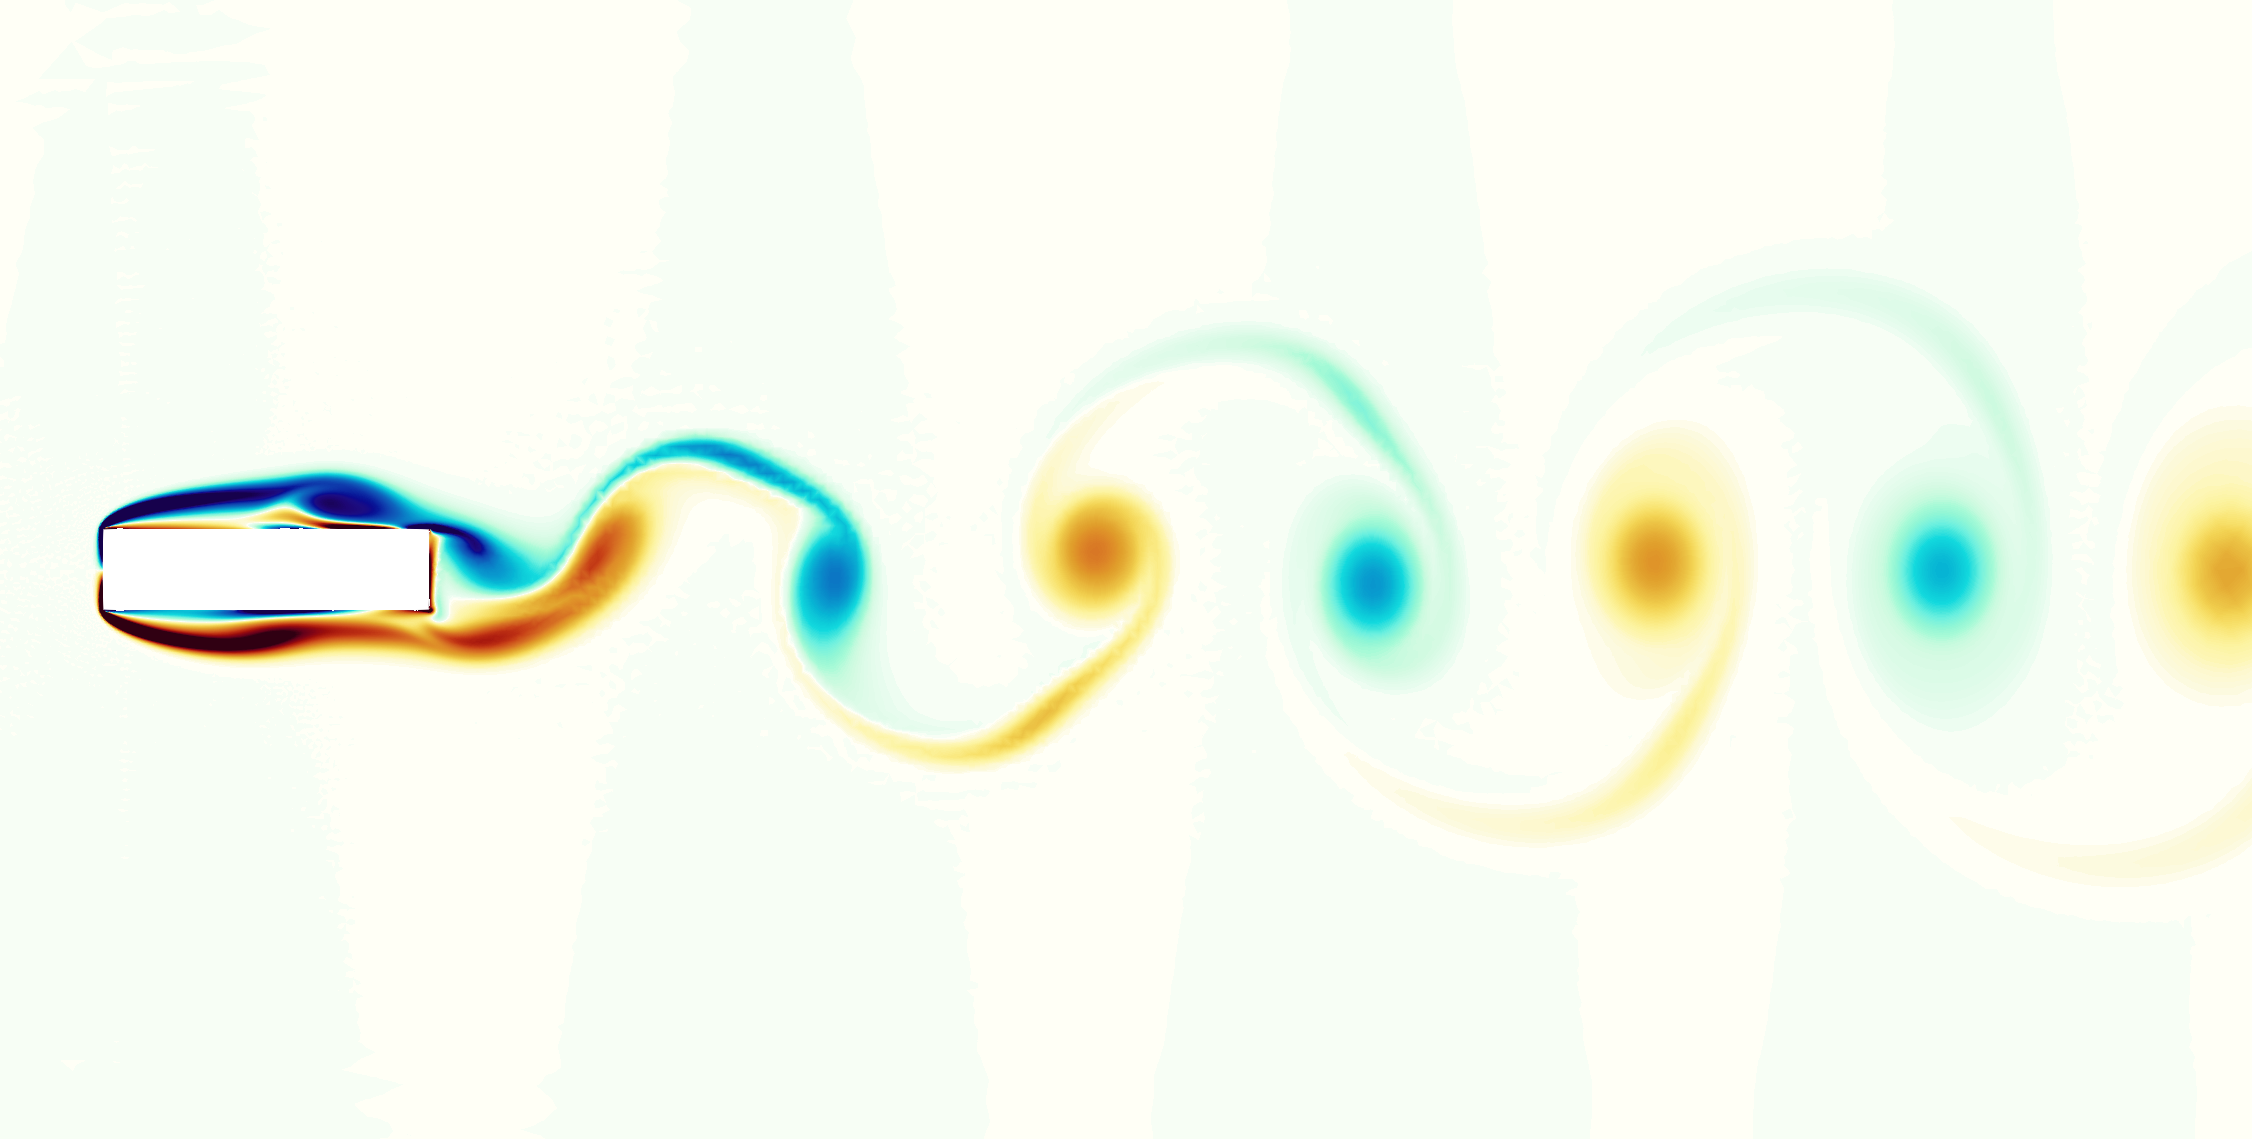
\includegraphics[trim={0 100 0 100},clip,width=0.49\textwidth]{./fig/vort_Re425_25.png}
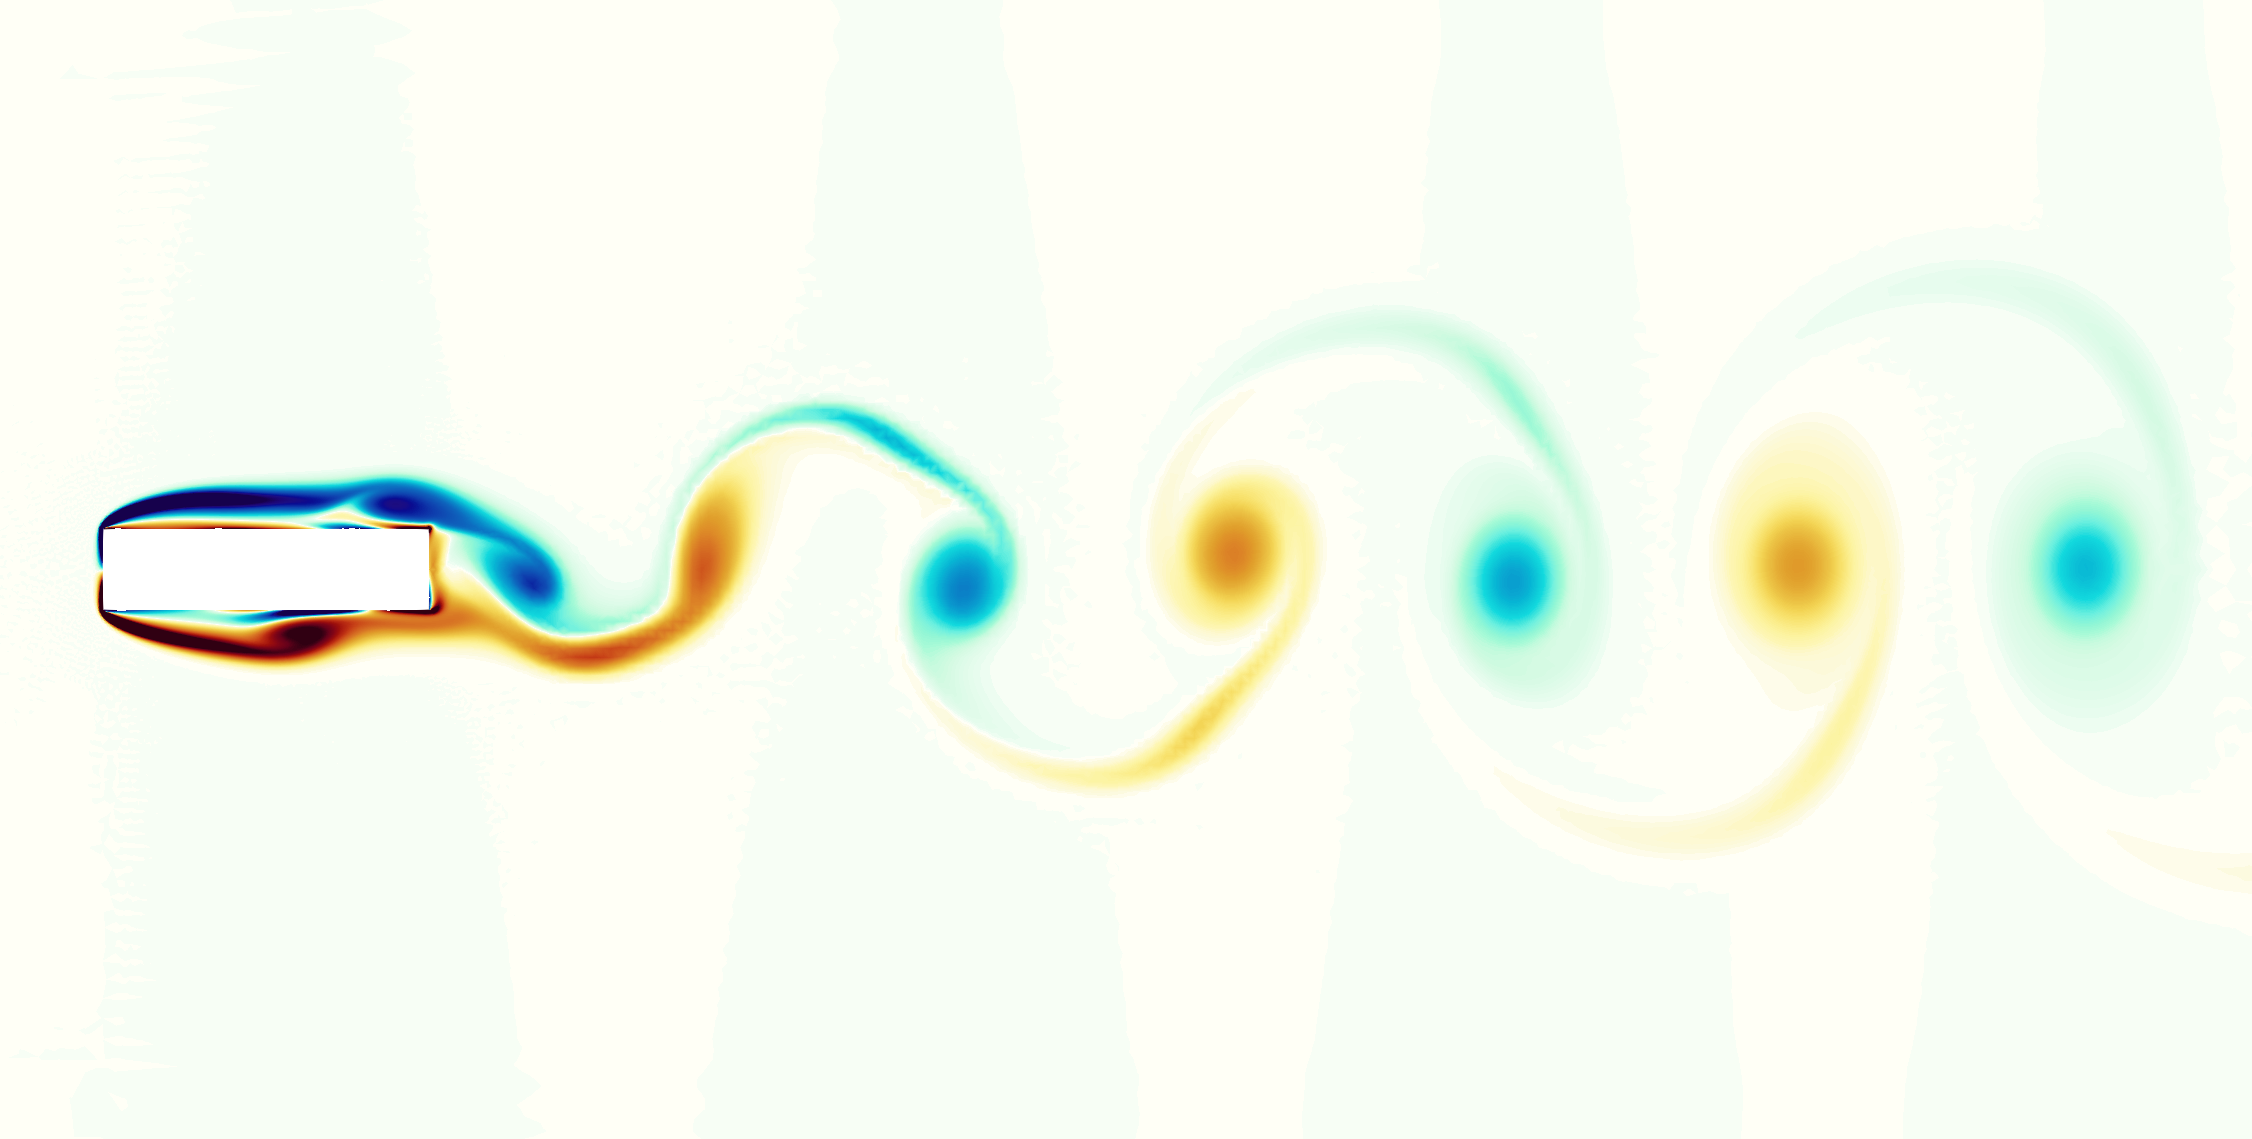
\includegraphics[trim={0 100 0 100},clip,width=0.49\textwidth]{./fig/vort_Re425_50.png}
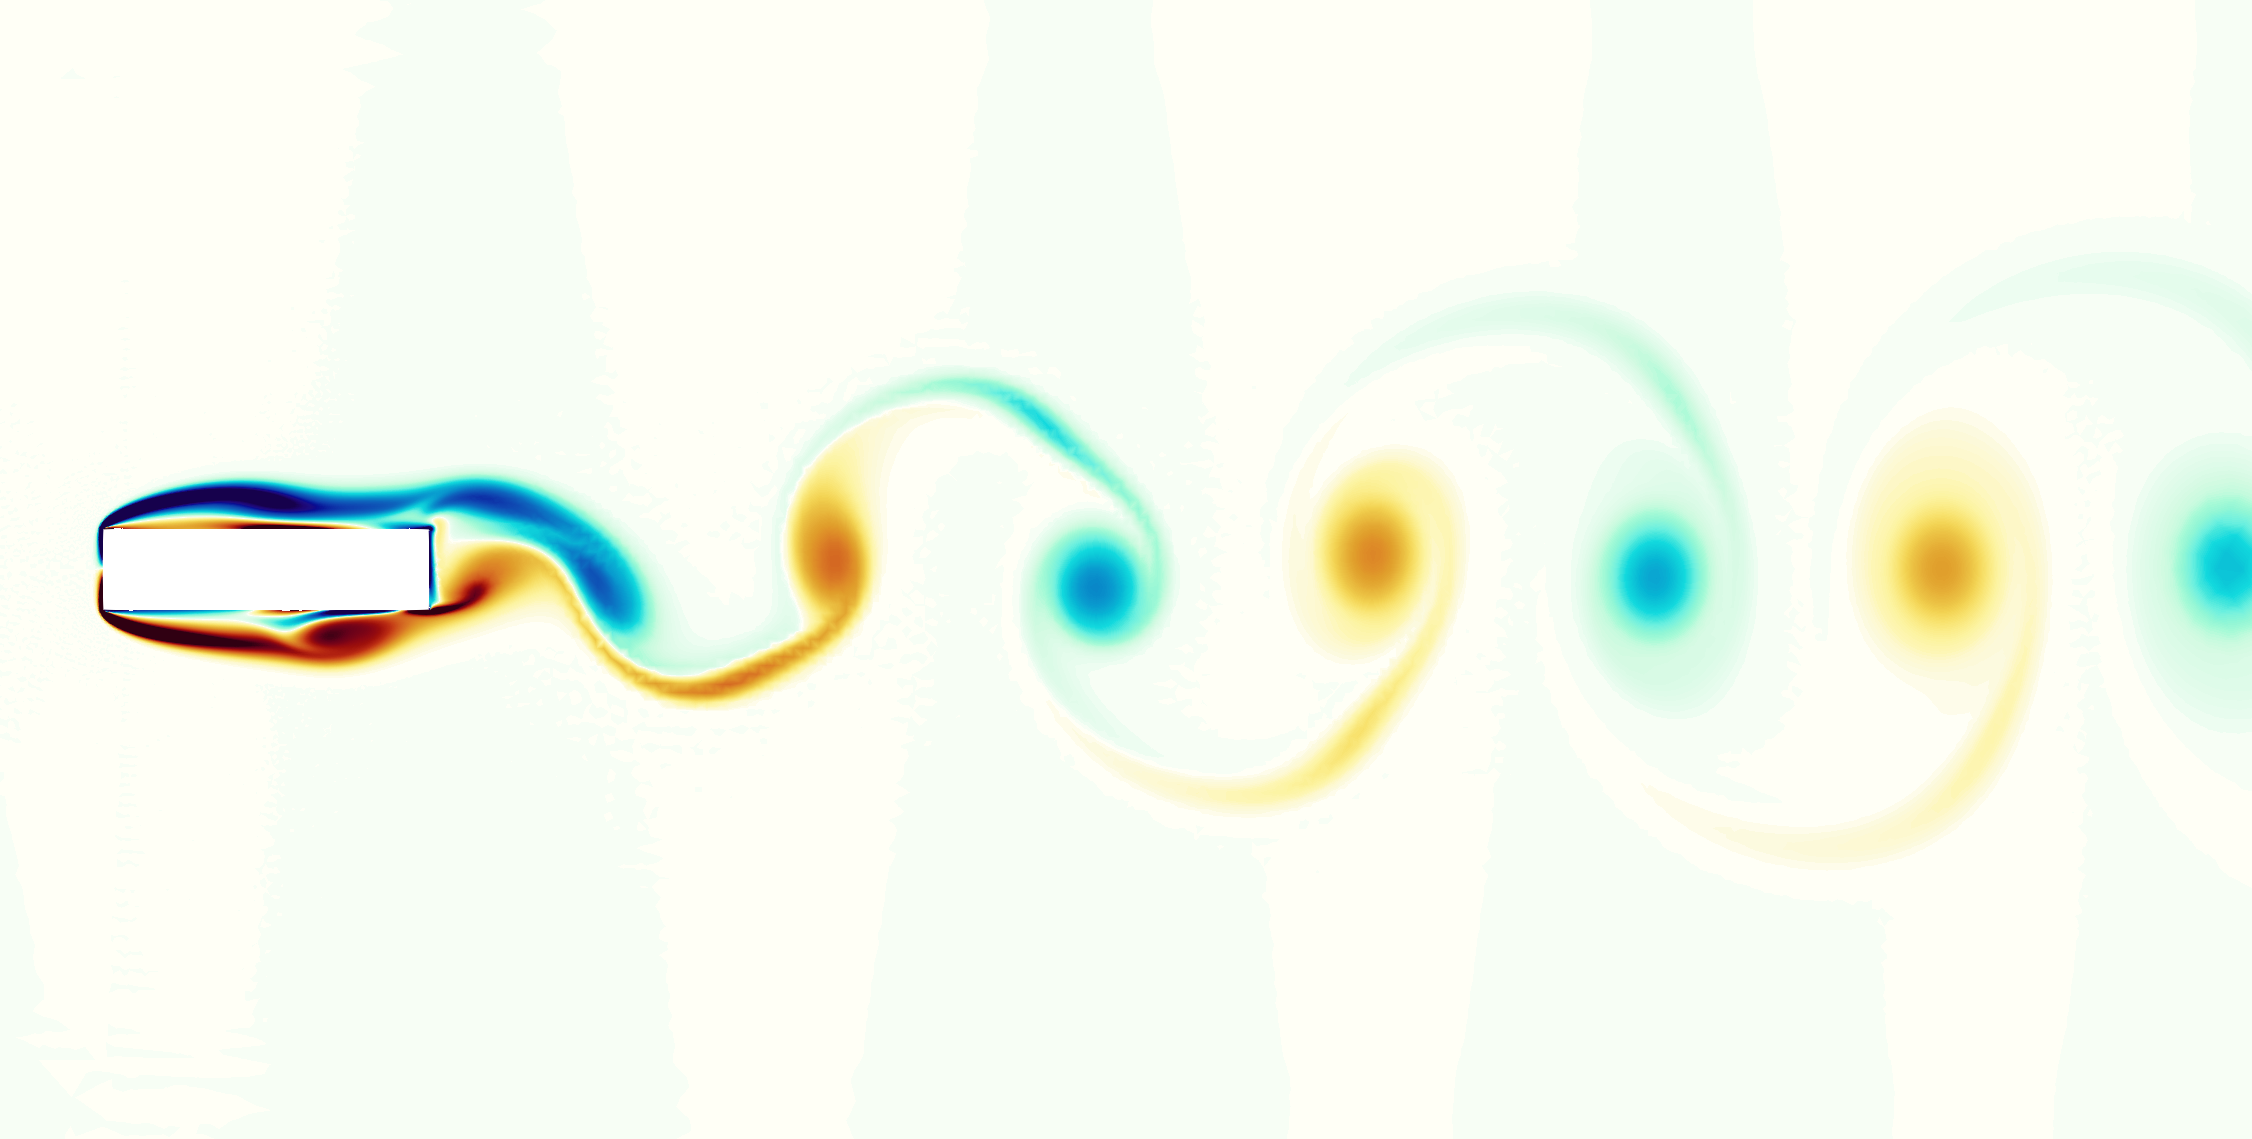
\includegraphics[trim={0 100 0 100},clip,width=0.49\textwidth]{./fig/vort_Re425_75.png}
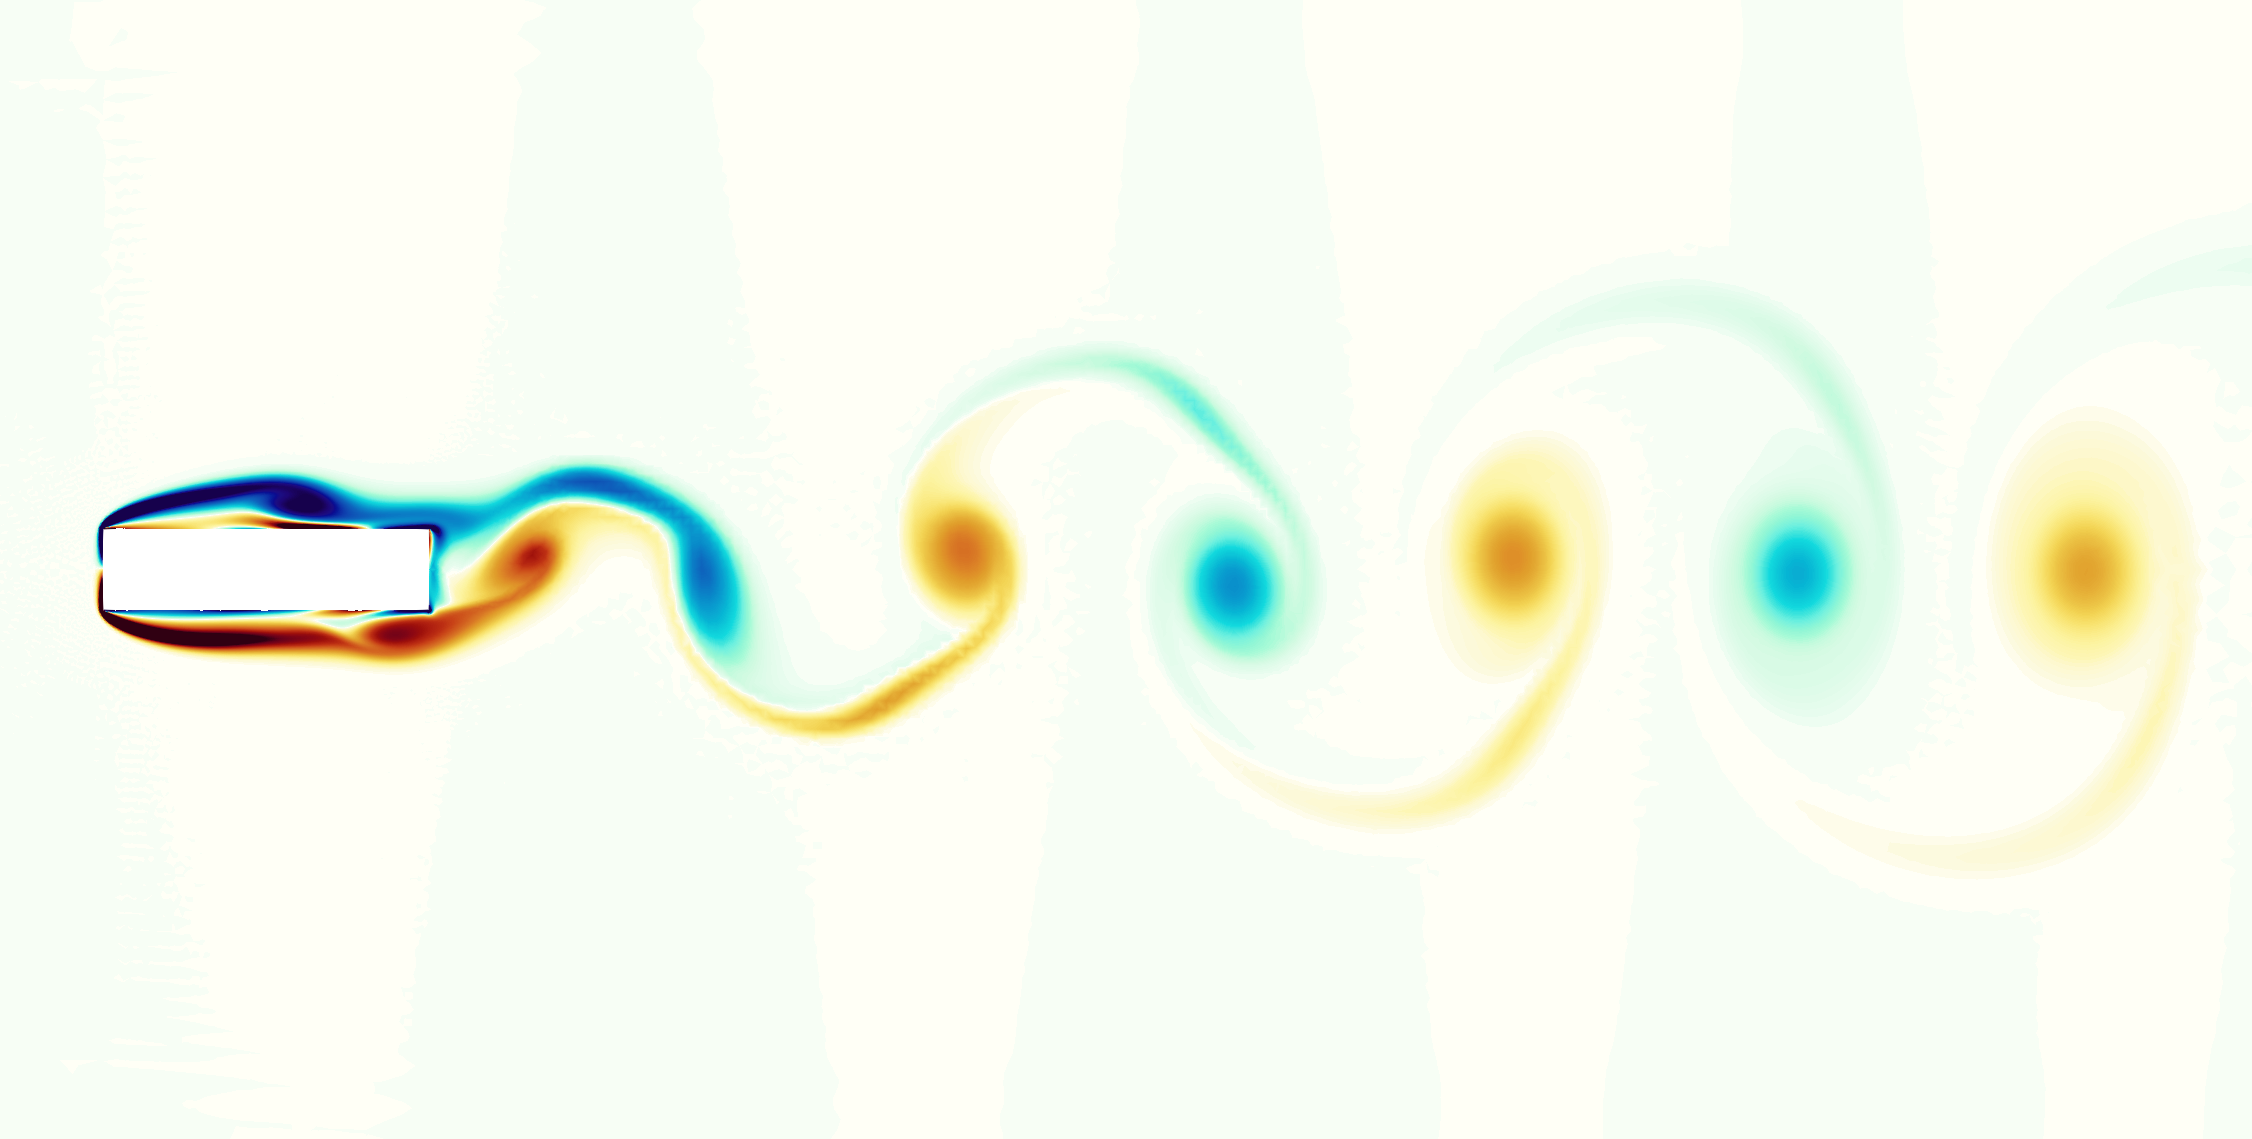
\includegraphics[trim={0 100 0 100},clip,width=0.49\textwidth]{./fig/vort_Re425_100.png}
\vspace{0.1cm}
\begin{tikzpicture}
\draw (-10,2) -- (8,2);
\end{tikzpicture}
\vspace{0.1cm}
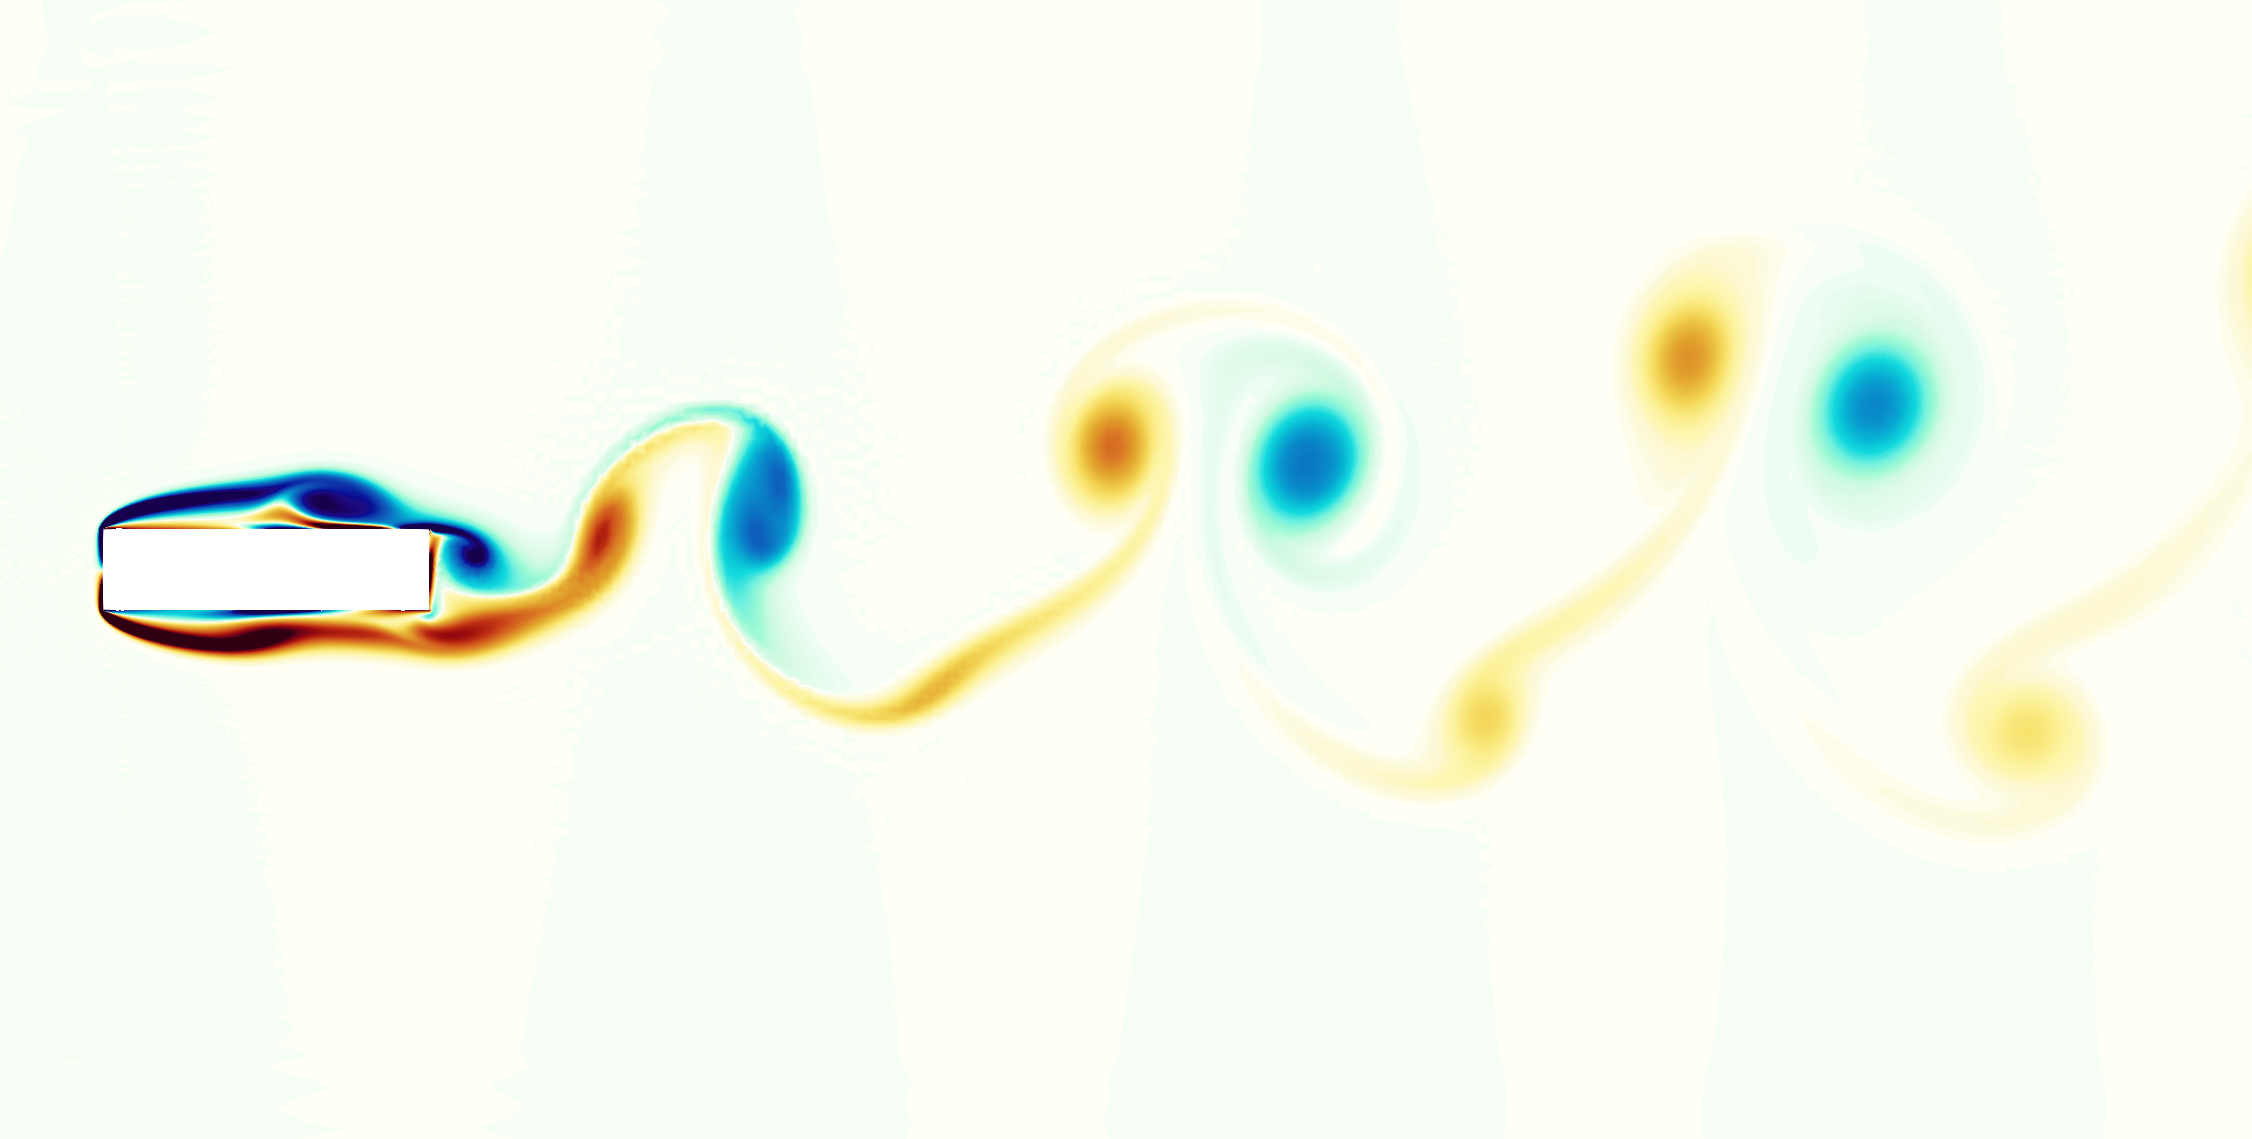
\includegraphics[trim={0 100 0 100},clip,width=0.49\textwidth]{./fig/vort_Re450_25.png}
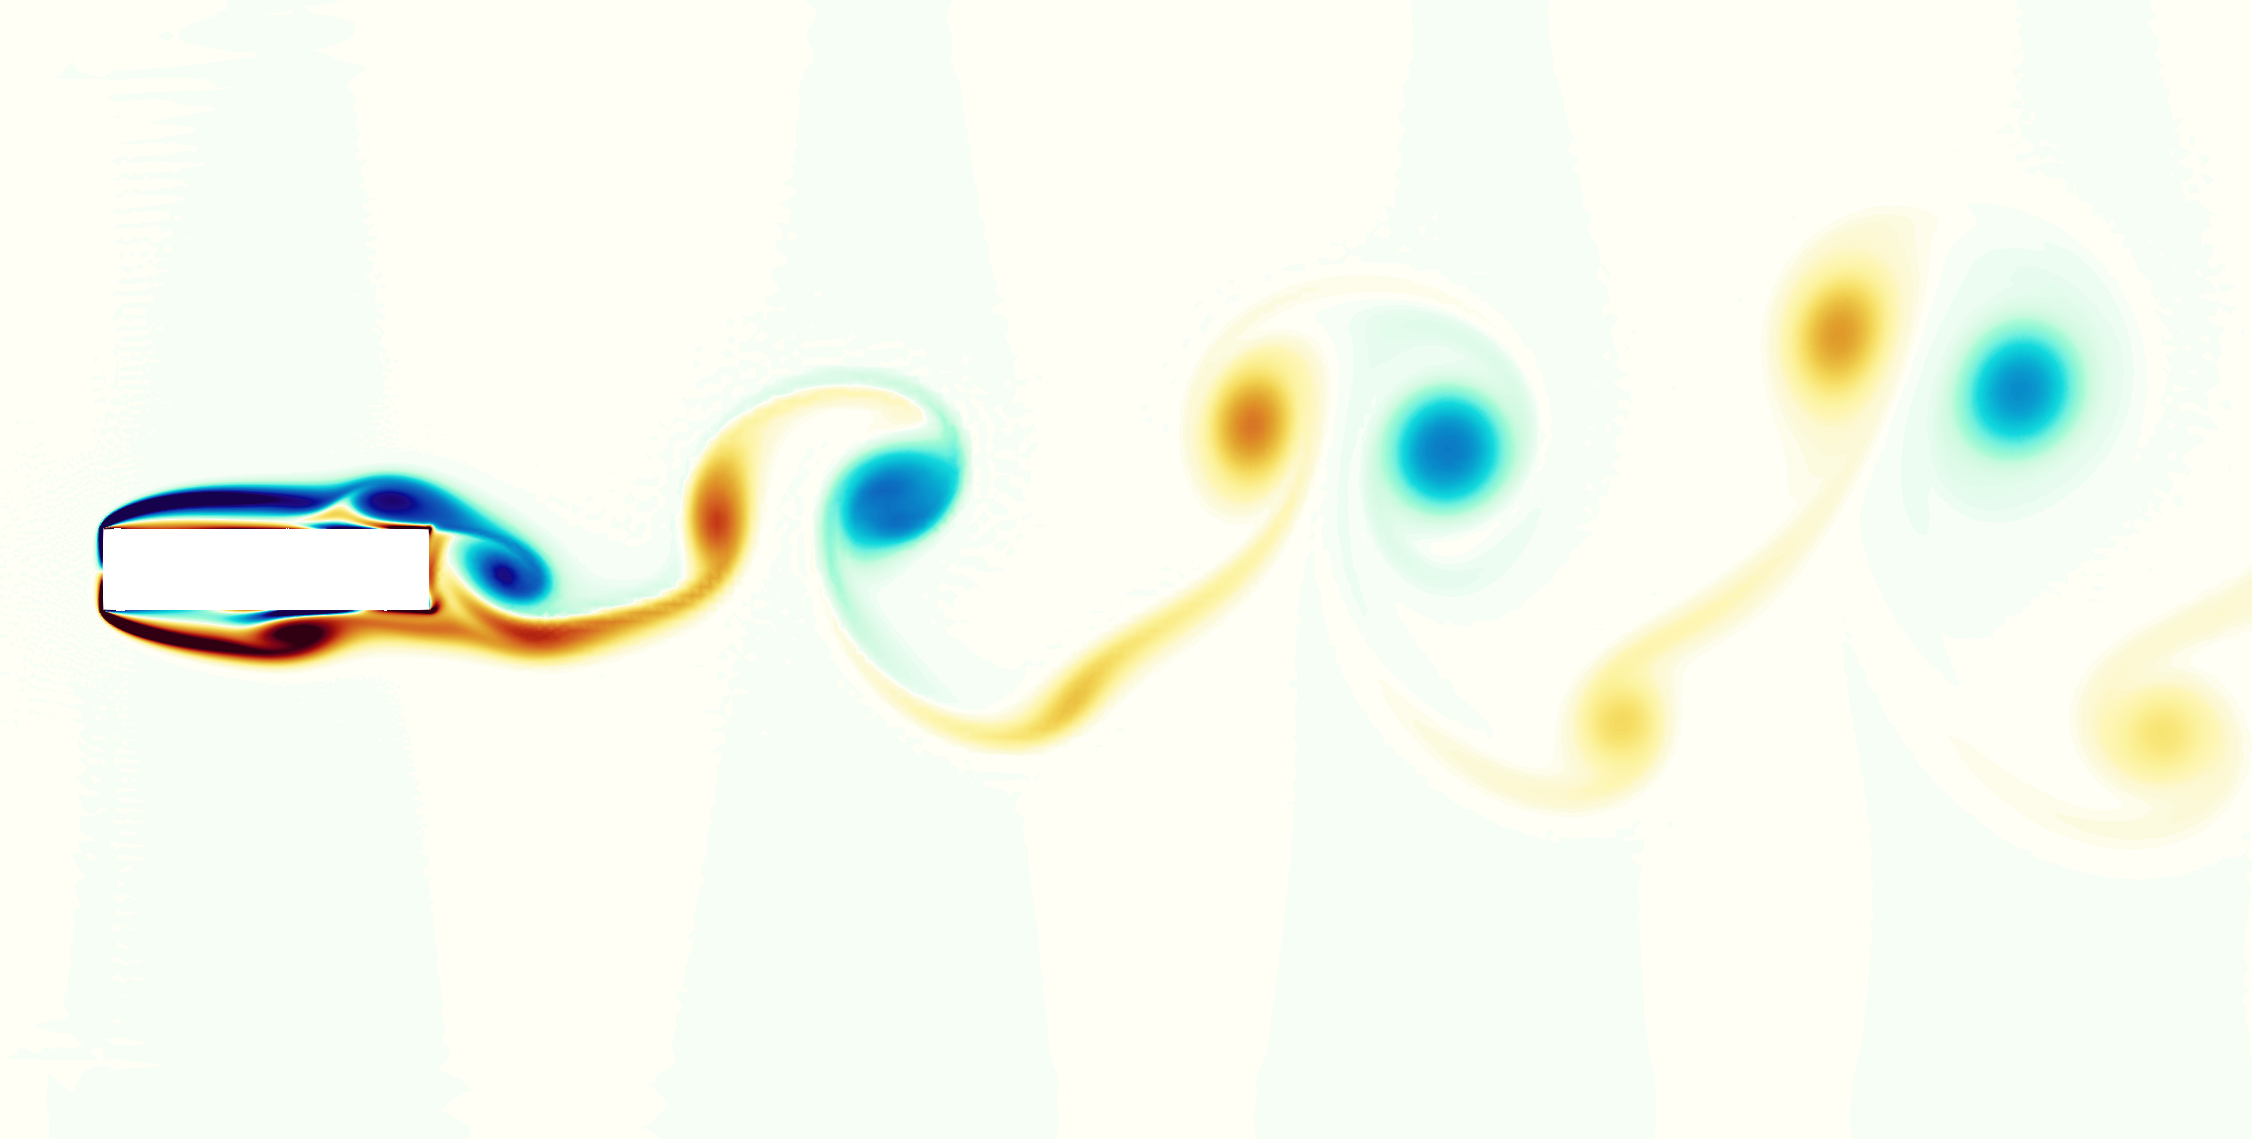
\includegraphics[trim={0 100 0 100},clip,width=0.49\textwidth]{./fig/vort_Re450_50.png}
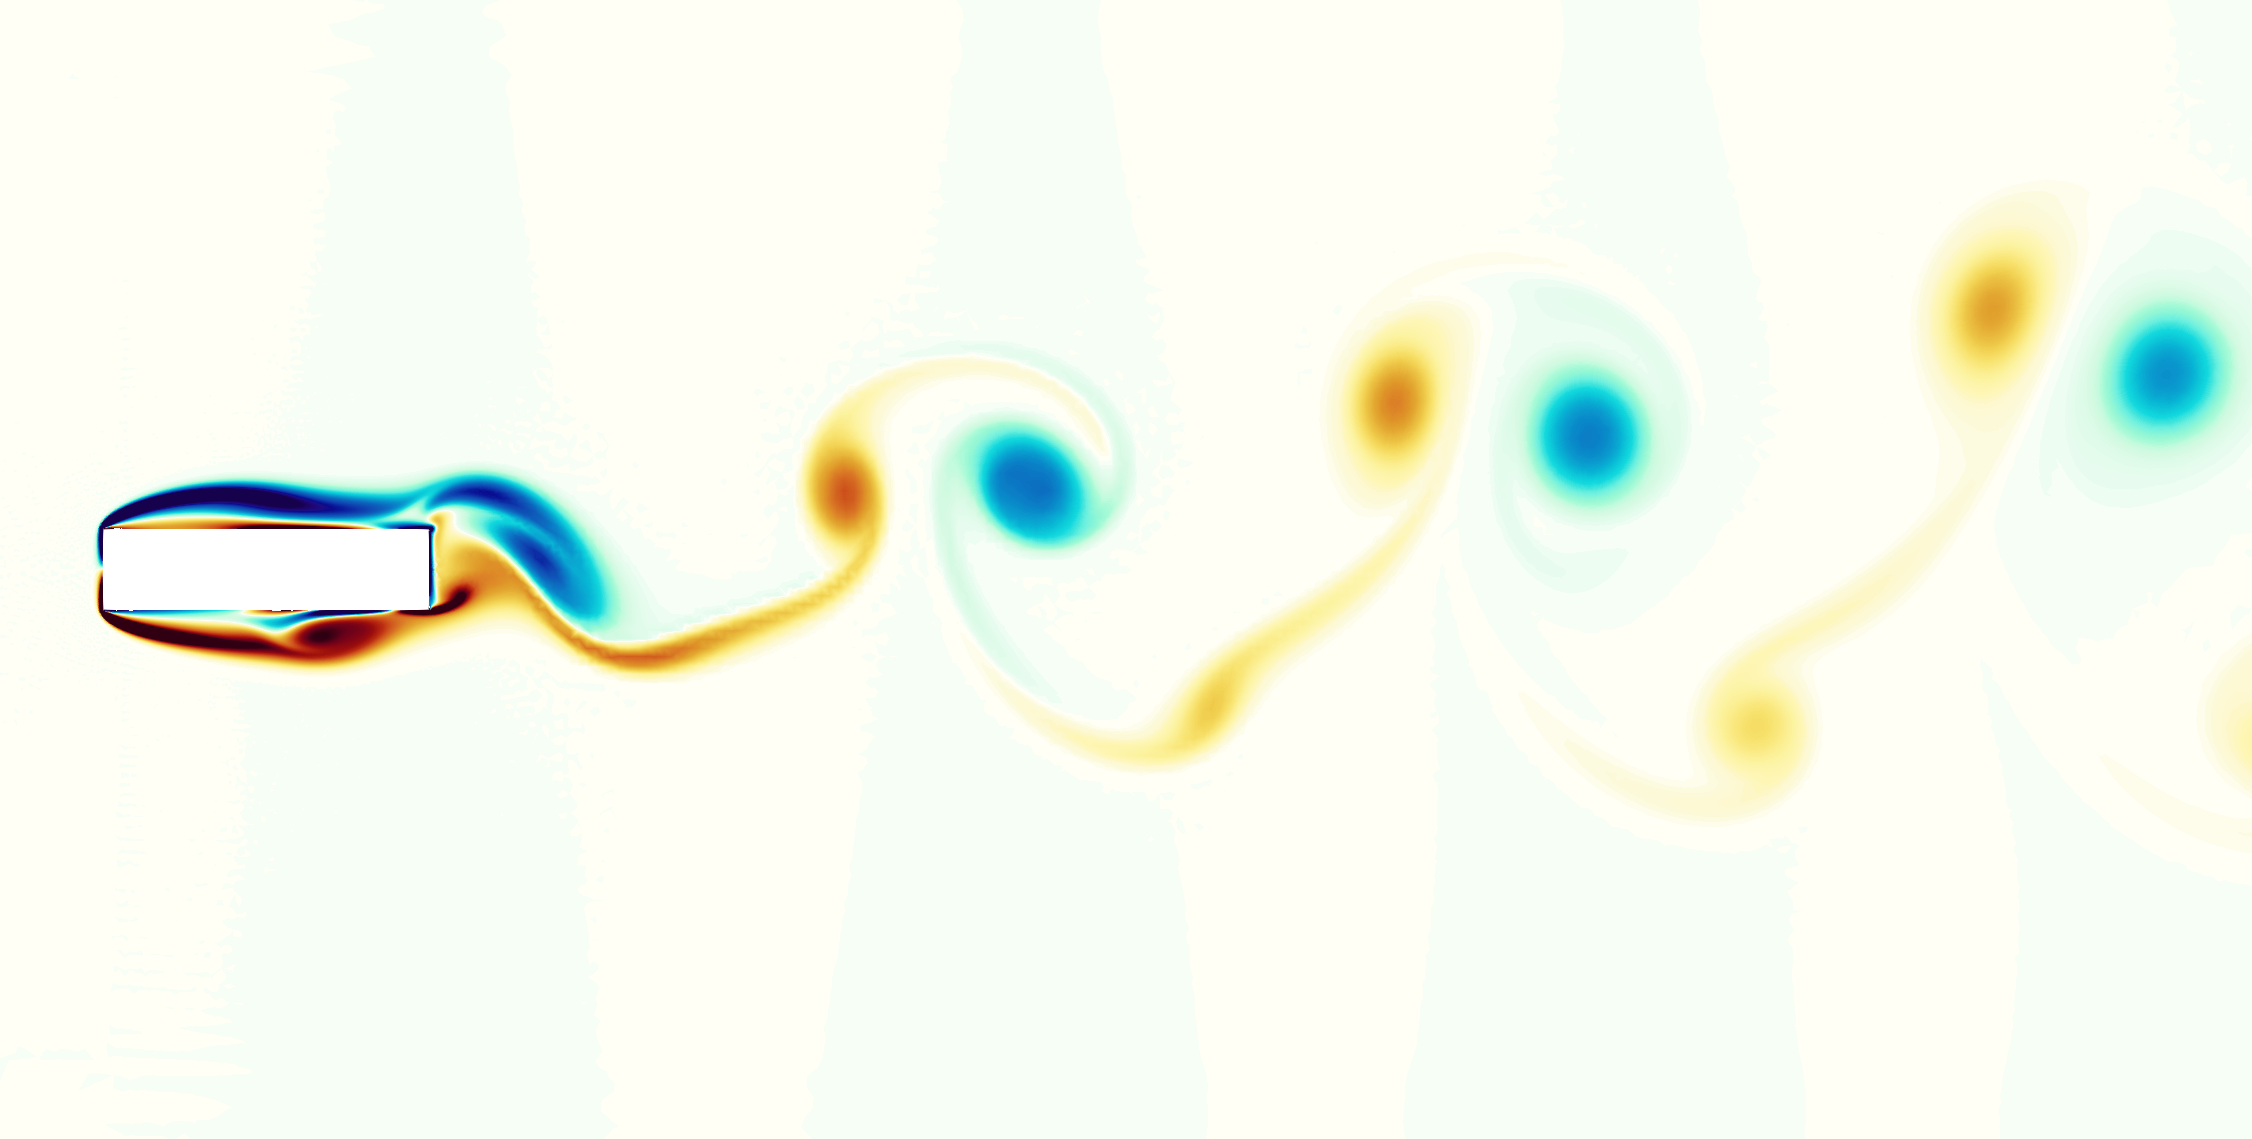
\includegraphics[trim={0 100 0 100},clip,width=0.49\textwidth]{./fig/vort_Re450_75.png}
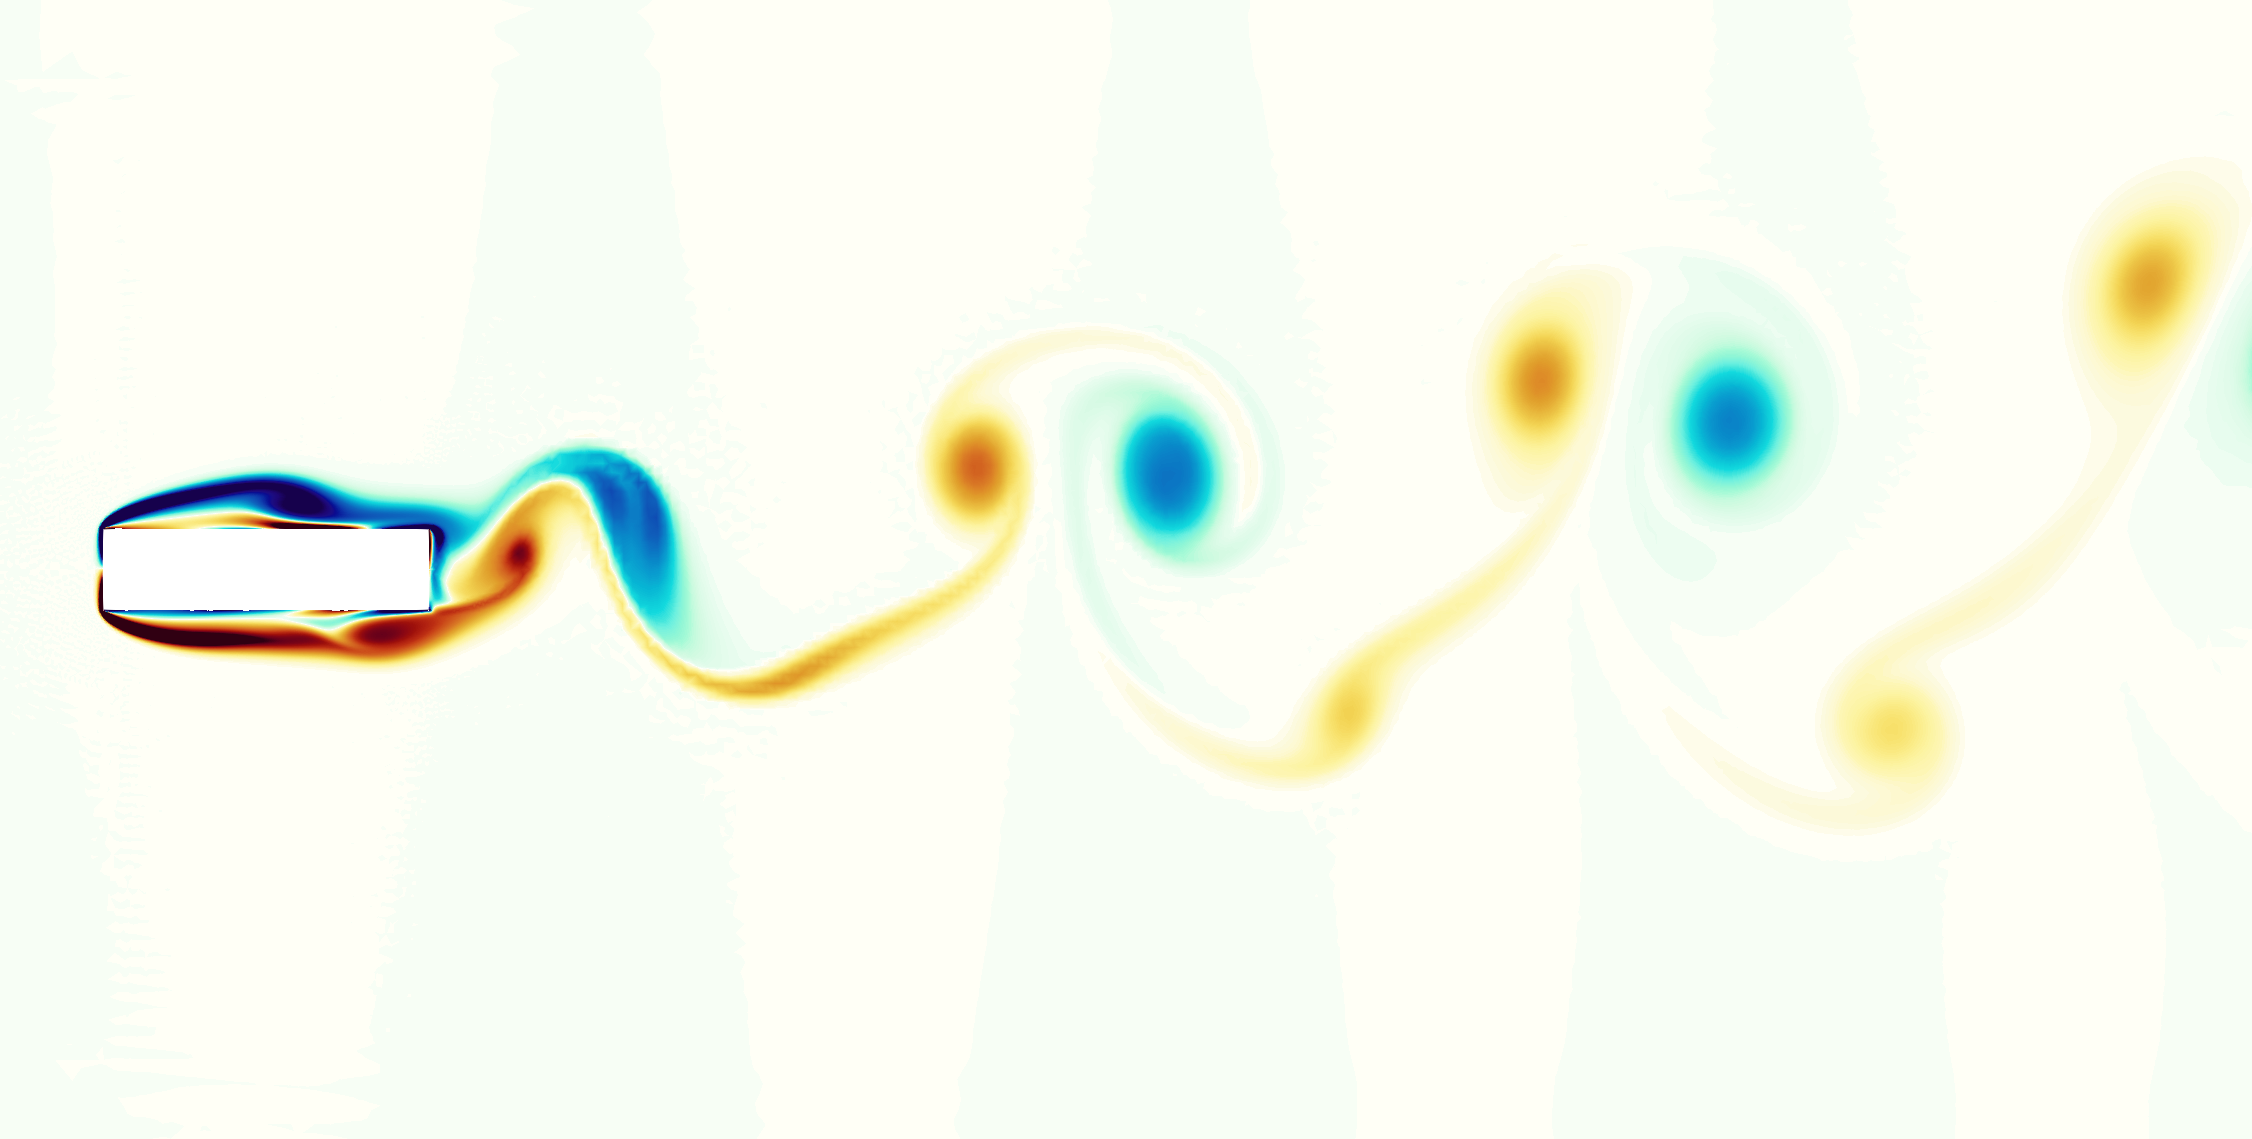
\includegraphics[trim={0 100 0 100},clip,width=0.49\textwidth]{./fig/vort_Re450_100.png}
\caption{Top: Evolution of the vorticity in one oscillation period for $\AR=4$ and $Re=425$. Bottom: Evolution of the vorticity in one oscillation period for $\AR=4$ and $Re=450$.}
\label{fig:vort_AR4_Re425}
\end{figure}

\begin{figure}
\centering
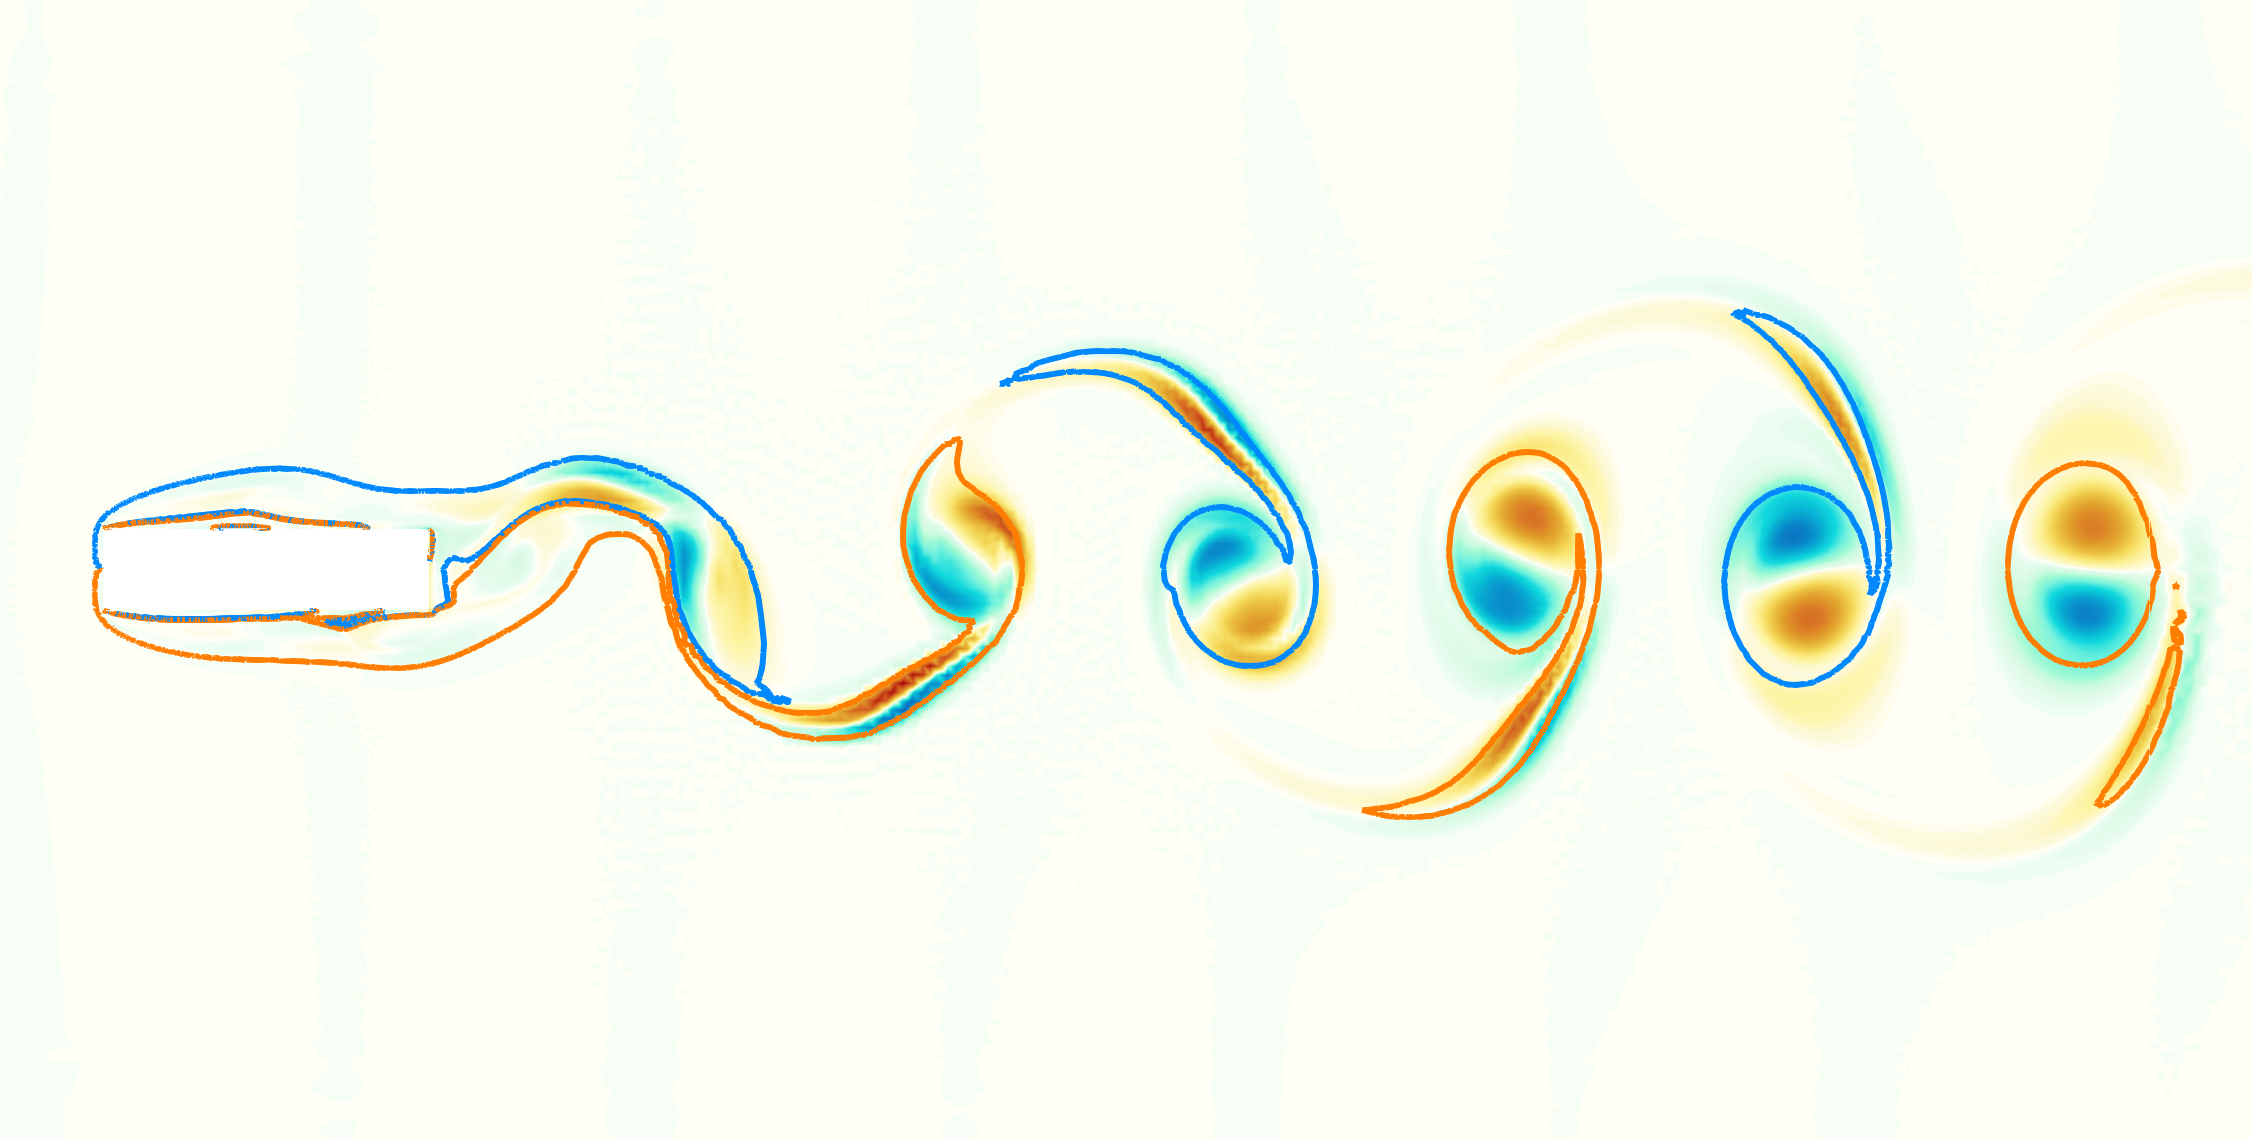
\includegraphics[trim={0 200 0 200},clip,width=0.7\textwidth]{./fig/omegaz_beta0_Re425.png}
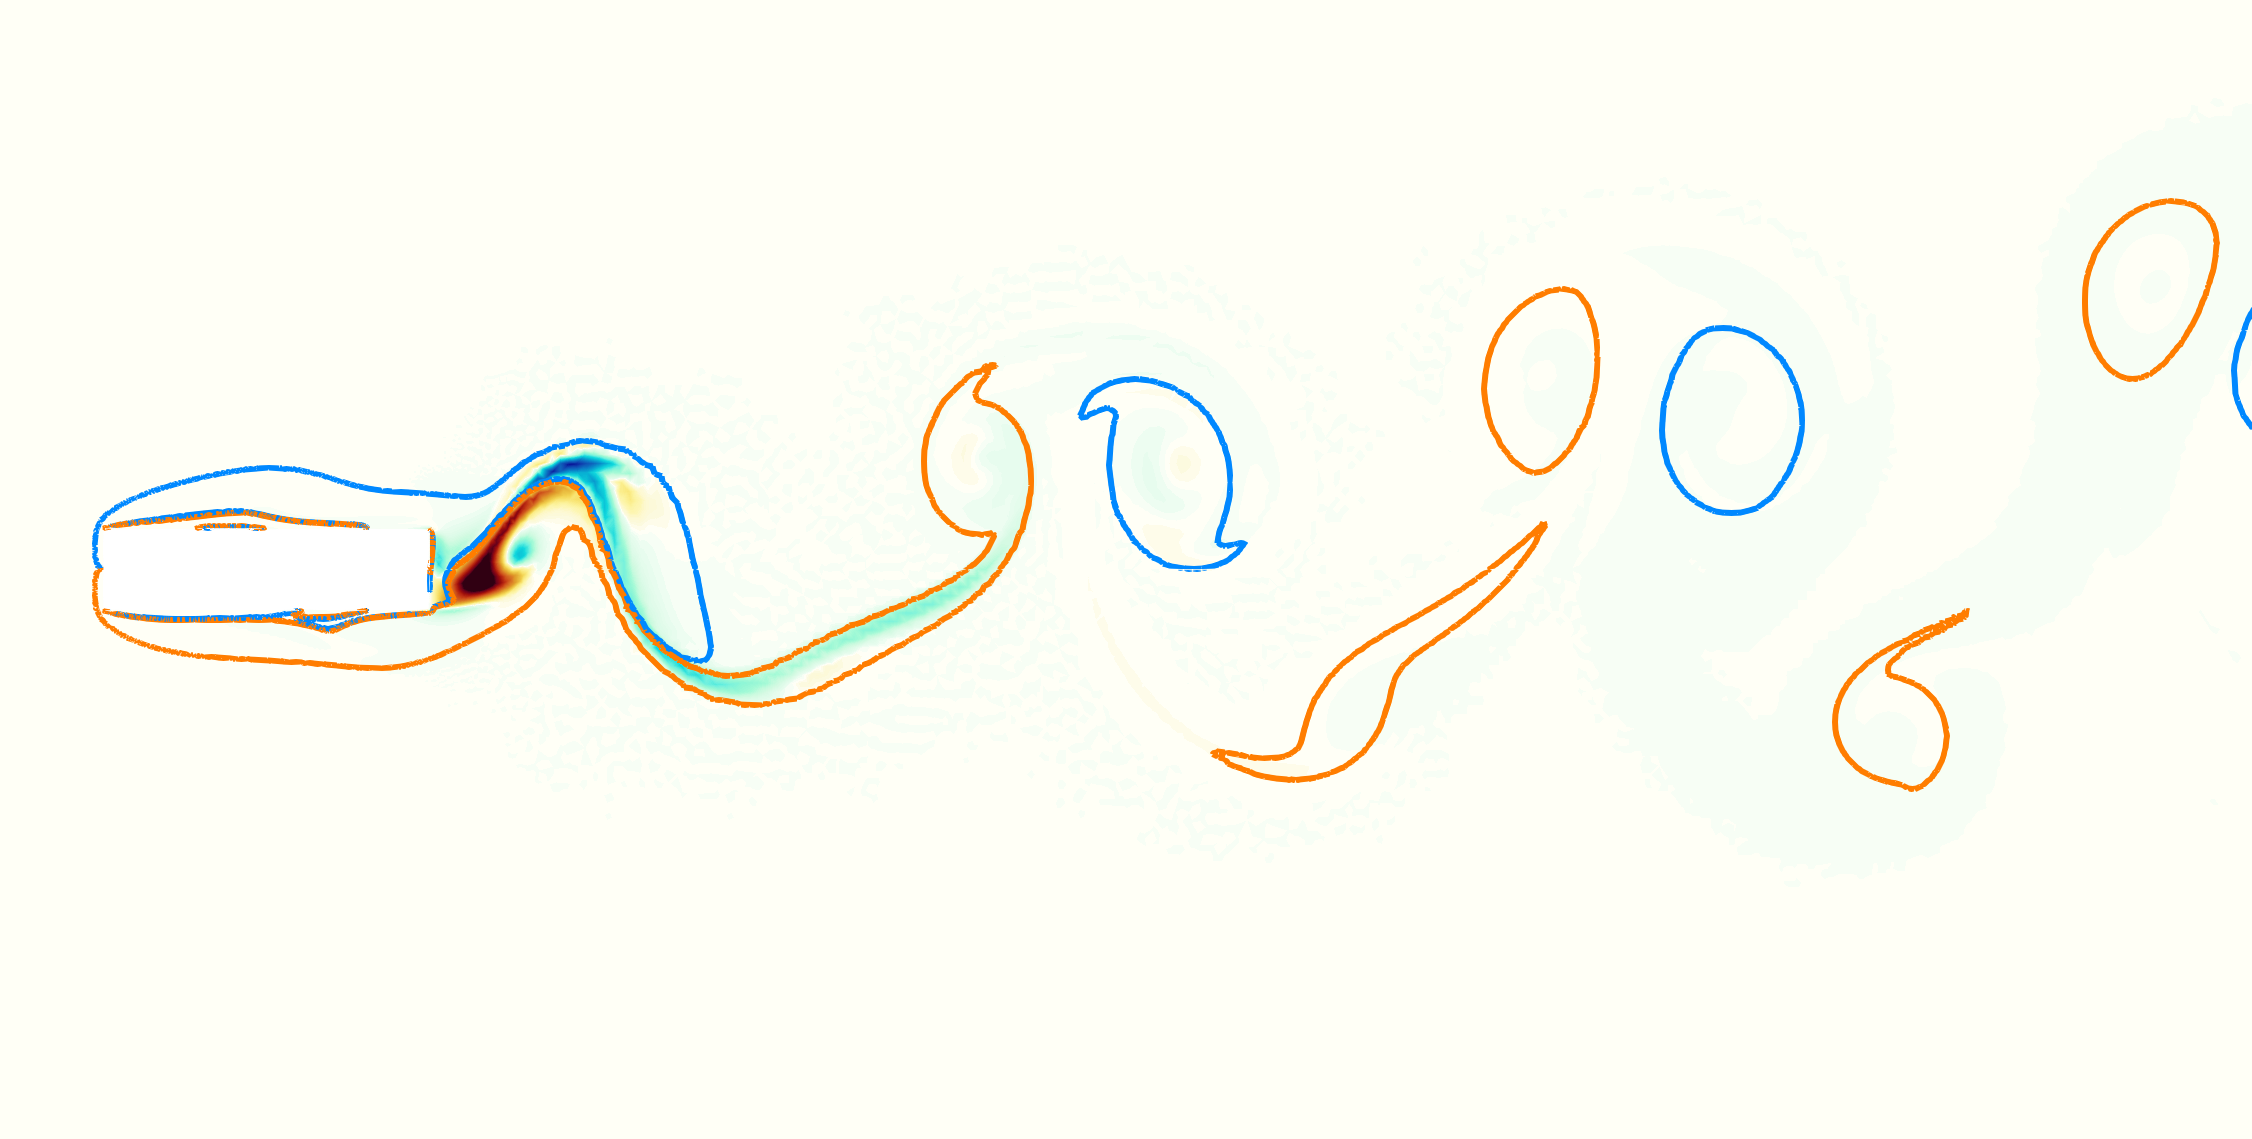
\includegraphics[trim={0 200 0 200},clip,width=0.7\textwidth]{./fig/omegaz_beta7p5_Re450.png}
\caption{Top: Floquet mode $\hat{\omega}_z$ for $\AR=4$, $Re=425$ and $\beta=0$. The isolines are vorticity of the base flow. Bottom: Floquet mode $\hat{\omega}_z$ for $\AR=4$, $Re=450$ and $\beta=7.5$. The isolines are vorticity of the base flow.}
\label{fig:AR4_Floquet_modes}
\end{figure}

\begin{figure}
\centering
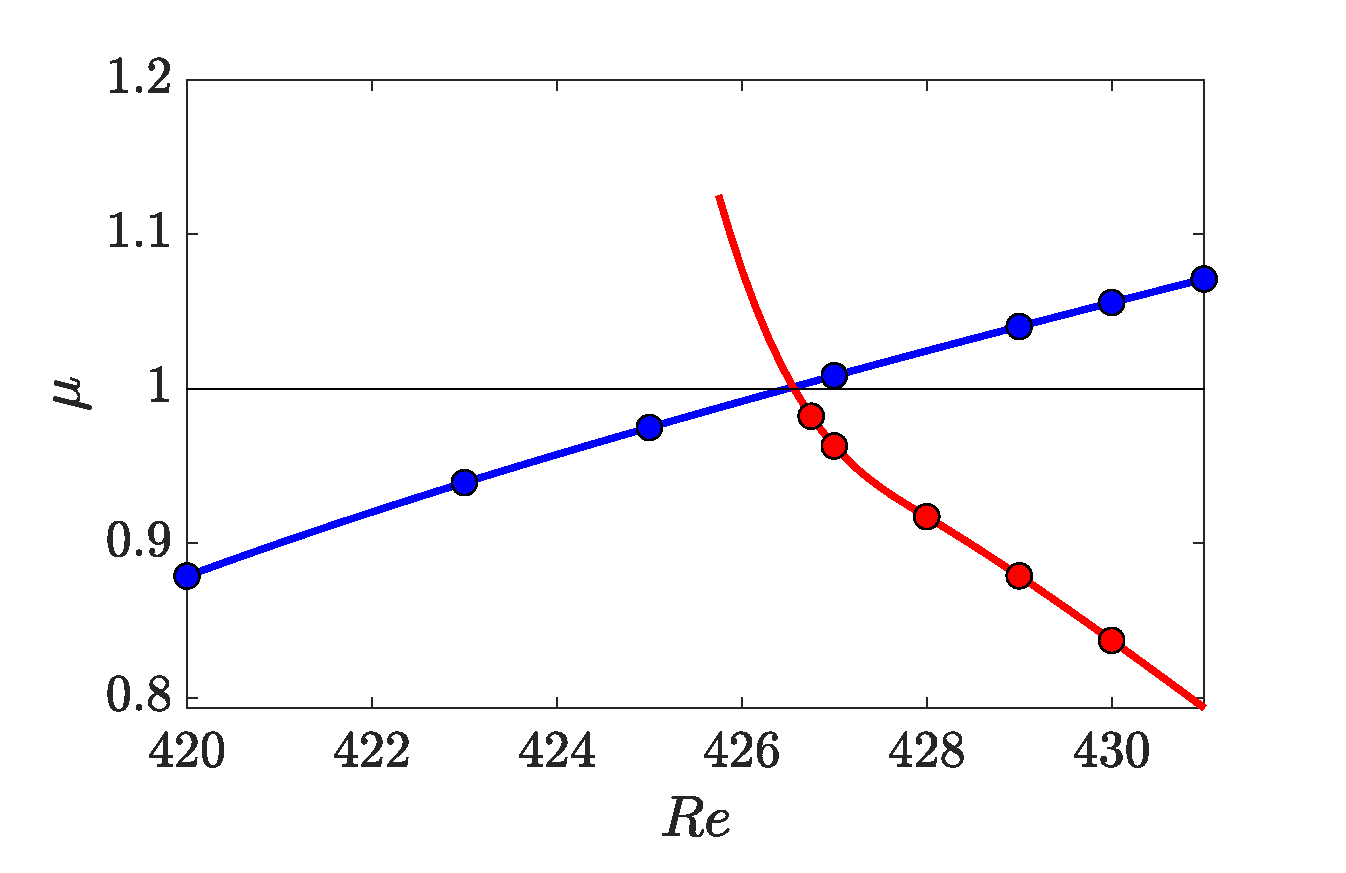
\includegraphics[width=0.49\textwidth]{./fig/AR4_2Dbif_multipliers.eps}
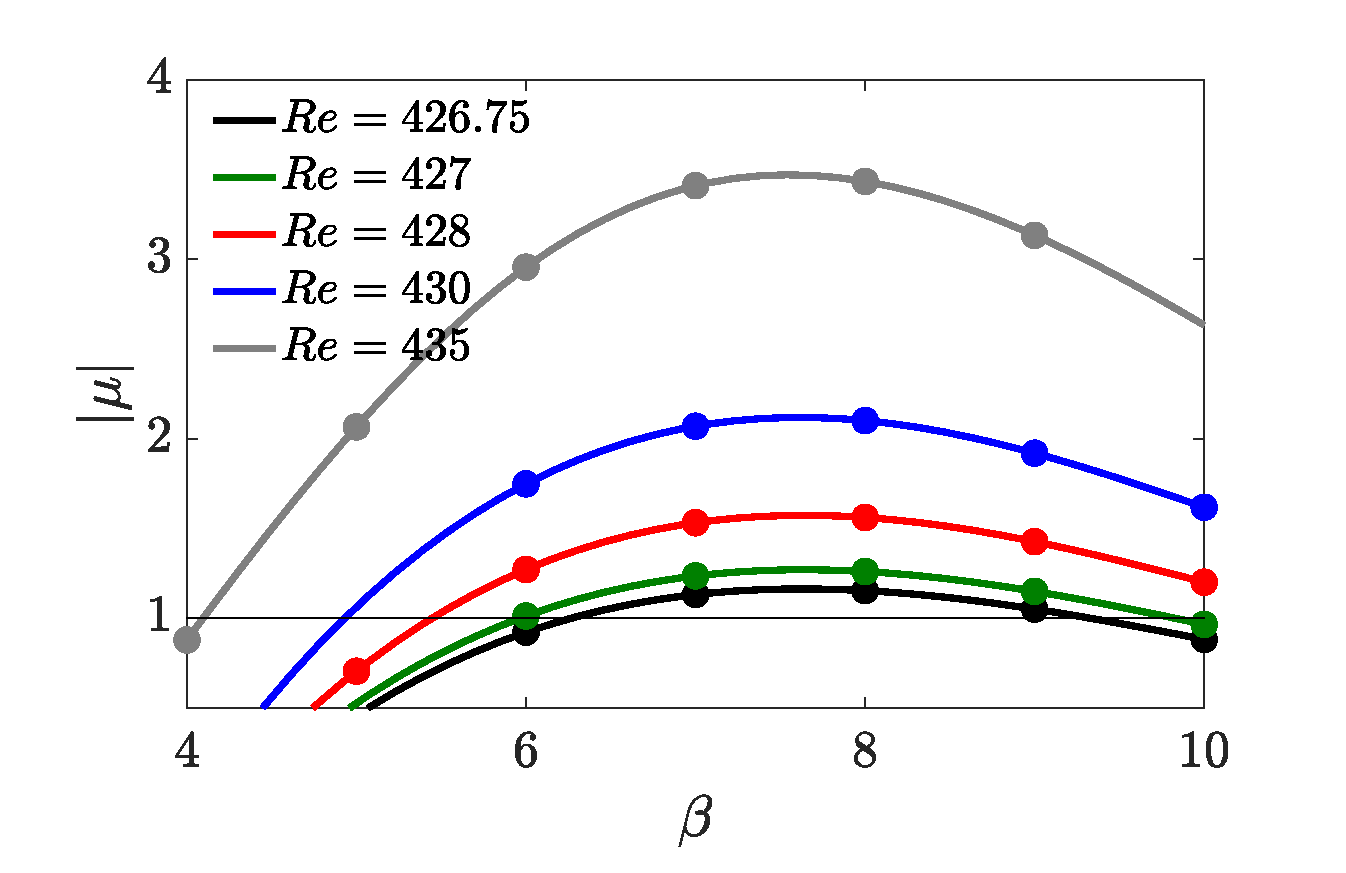
\includegraphics[width=0.49\textwidth]{./fig/AR4_3Dbif_multipliers.eps}
\caption{Left: Stability margin for the straight and slanted wake configuration. The blue circles are the Floquet multipliers related to the base flow with straight wake configuration. The red circles are the Floquet multipliers related to the base flow with the slanted wake configuration. Right: Stability of the slanted wake configuration to three-dimensional perturbations. Modulus of the Floquet unstable floquet multipliers. {\color{red} Need to check the dependence of the results on the size of the computational domain}.}
\label{fig:2Dmultipliers}
\end{figure}

We start considering $\AR=4$, which is in the first horizontal branch of the $St-\AR$ curve. We observe that the flow regime changes as $Re$ increases. For $Re \le 425$ the flow is periodic and the wake is straight. For larger $Re$, instead, the wake experiences an additional bifurcation and becomes slanted. For this $\AR$, the flow experiences a secondary two-dimensional bifurcation towards a limit cycle with the same frequency, before becoming three-dimensional. This is visualised in figures \ref{fig:vort_AR4_Re425} and \ref{fig:vort_AR4_Re450} where flow snapshots are shown for $Re=425$ and $Re=450$. For the lowest $Re$ the wake is straight and characterised by the usual alternating shedding of vortices with positive/negative vorticity from the bottom/top sides of the cylinder. Note that vortices are shed also from the LE, and in agreement with previous results in literature, a single vortex is place at each time over the lateral sides. At $Re=450$, instead, we find a slanted wake. In this case, indeed, the vortex monopoles are not placed along the $y=0$ line, but progressively deviate a part. This has been observed for $Re \ge 435$. 

To investigate the origin of this phenomenon, we have studied the linear stability of the straight wake to two-dimensional perturbations, using Floquet theory; see figure \ref{fig:2Dmultipliers}. For $Re=425$ we have found a multiplier that is very lose to the unit circle being $\mu \approx (0.97,0)$. This agrees with the fact that at this $Re$ the straight wake is stable and that it becomes unstable at slightly larger $Re$. Also, the fact that $\Im(\mu)= 0$ confirms the fact that the slanted wake is the result of a synchronous global instability of the wake. To provide further details, in the top panel of figure \ref{fig:AR4_Floquet_modes} we show the structure of the Floquet mode with isolines of the base-flow vorticity. In the wake the unstable mode generates dipoles of spanwise vorticity that grow in space and time as they are advected downstream. A synchronisation between the base flow and the perturbation field is observed, with the dipoles of the linear mode being centred with the the base-flow vortices at all times. %
A dipolar perturbation of a monopolar vortex is often referred to as displacement mode \citep{brion-sipp-jacquin-2014} and is known to result in a displacement of the vorticity centroid, similarly to what observed in figure \ref{fig:vort_AR4_Re450}. We consider the first positive base-flow vorticity monopole in the wake. Here the Floquet dipole has positive vorticity in the upper part, and negative vorticity in the lower part. This superposition strengthens the top part of the monopole and weakens the bottom part, resulting into a net displacement of the monopole in the upward direction. In contrast, in the second monopole of negative base-flow vorticity the scenario is the opposite. The Floquet dipole has positive vorticity in the bottom part of the monopole, and negative vorticity in the top part %. This strengthens the top part of the monopole and weaken the bottom part, and result
resulting again into a upward shift of the monopole. This explains the vertical displacement of the vortex centroids shown in figure \ref{fig:vort_AR4_Re450}. Overall, this mechanism resembles what observed in \cite{jallas-marquet-fabre-2017} in the case of pitching airfoils.


%
Notably, this new slanted wake is strongly unstable to three-dimensional perturbations of subharmonic nature, being characterised by a small spanwise wavelenght (a large value of $\beta$); see figure \ref{fig:2Dmultipliers}. The linear stability of the slanted wake to three-dimensional perturbations has been investigated again by mean of Floquet analysis. For $Re \ge 435$ we have found a Floquet multiplier outside the unit circle, having negative imaginary part. For $Re=450$ we found $ mu \approx (-4.8,0)$ for $\beta=7$ ({\color{red} we still have to study the dependence of the results on the vertical extent of the computational domain}). The 
structure of the mode is shown in the bottom panel of figure \ref{fig:AR4_Floquet_modes}. This is clearly an unstable mode of the wake. The mode, indeed, in almost null over the lateral sides of the cylinder where instead the flow dynamics is driven by the vortices shed by the LE.




\begin{itemize}
  \item It is still not clear whether the slanted wake is stable for a certain range of $Re$. It actually seems that when the wake becomes slanted it is immediately unstable to three-dimensional perturbations. How is it possible?
  \item After characterising the linear stability of the straight- and slanted-wake configuration it would be interesting to investigate the influence of the non linearity. We can follow the same approach proposed by \cite{jallas-marquet-fabre-2017}. We can stabilise the bifurcation, and write the non linear perturbation at a certain $Re$ as $\{ \bm{u}'',p'' \} = \{\bm{u},p \} - \{\bm{u}_S,p_S \}$, where we use the $\cdot_S$ subscript when referring to the symmetric configuration. At this point we have can plot the perturbation and discuss it. Also, we may also divide it is the symmetric and anisymmetric part to then address what is the influence of the two symmetric and asymmetric modes. Before doing this, we need to use BoostConv to symmetrise the flow, and compute the forces, to understand which is the question we want to address.
  \item Is the mechanism associated with the instability a viscous one? A possible approach would be to perform the Floquet stability by progressively increasing the $Re$?
  \item Also, why the flow becomes suddenly unstable to 3D perturbations once the wake becomes slanted? That mode is not present in the spectrum of the straight wake. My idea is that the feedback that leads to this mode is associated with something close to the trailing edge that appears only in this case. What about looking again at the close orbits, like Giannetti (2010)? We have already tried in a different set up, and we already have the code for this kind of computations.
  \item The scenario seems to hold also for $\AR=4.5$; see figure \ref{fig:vort_AR4p5_Re450}. Actually, in this case flow the low-$Re$ straight wake we observe two multipliers that approach the unit circle for $\beta=0$. One is real and positive (as for $\AR=4$), while one is complex. However, the structure of the mode is similar in both cases (see figure \ref{fig:AR4p5_modes_Re430_beta0}. For $Re=430$ they are $\mu = (1.249,0)$ and $\mu=(0.7949, \pm 0.52)$. Also, once the wake settles to the slanted configuration, similarly to what observed for $\AR=4$ we observe that it is strongly unstable to 3D perturbations with a small spanwise wavelength. Overall, this has been confirmed by Direct numerical simulations; see figure \ref{fig:lambda2_omegax_AR45_Re450}.
\end{itemize}

\begin{figure}
\centering
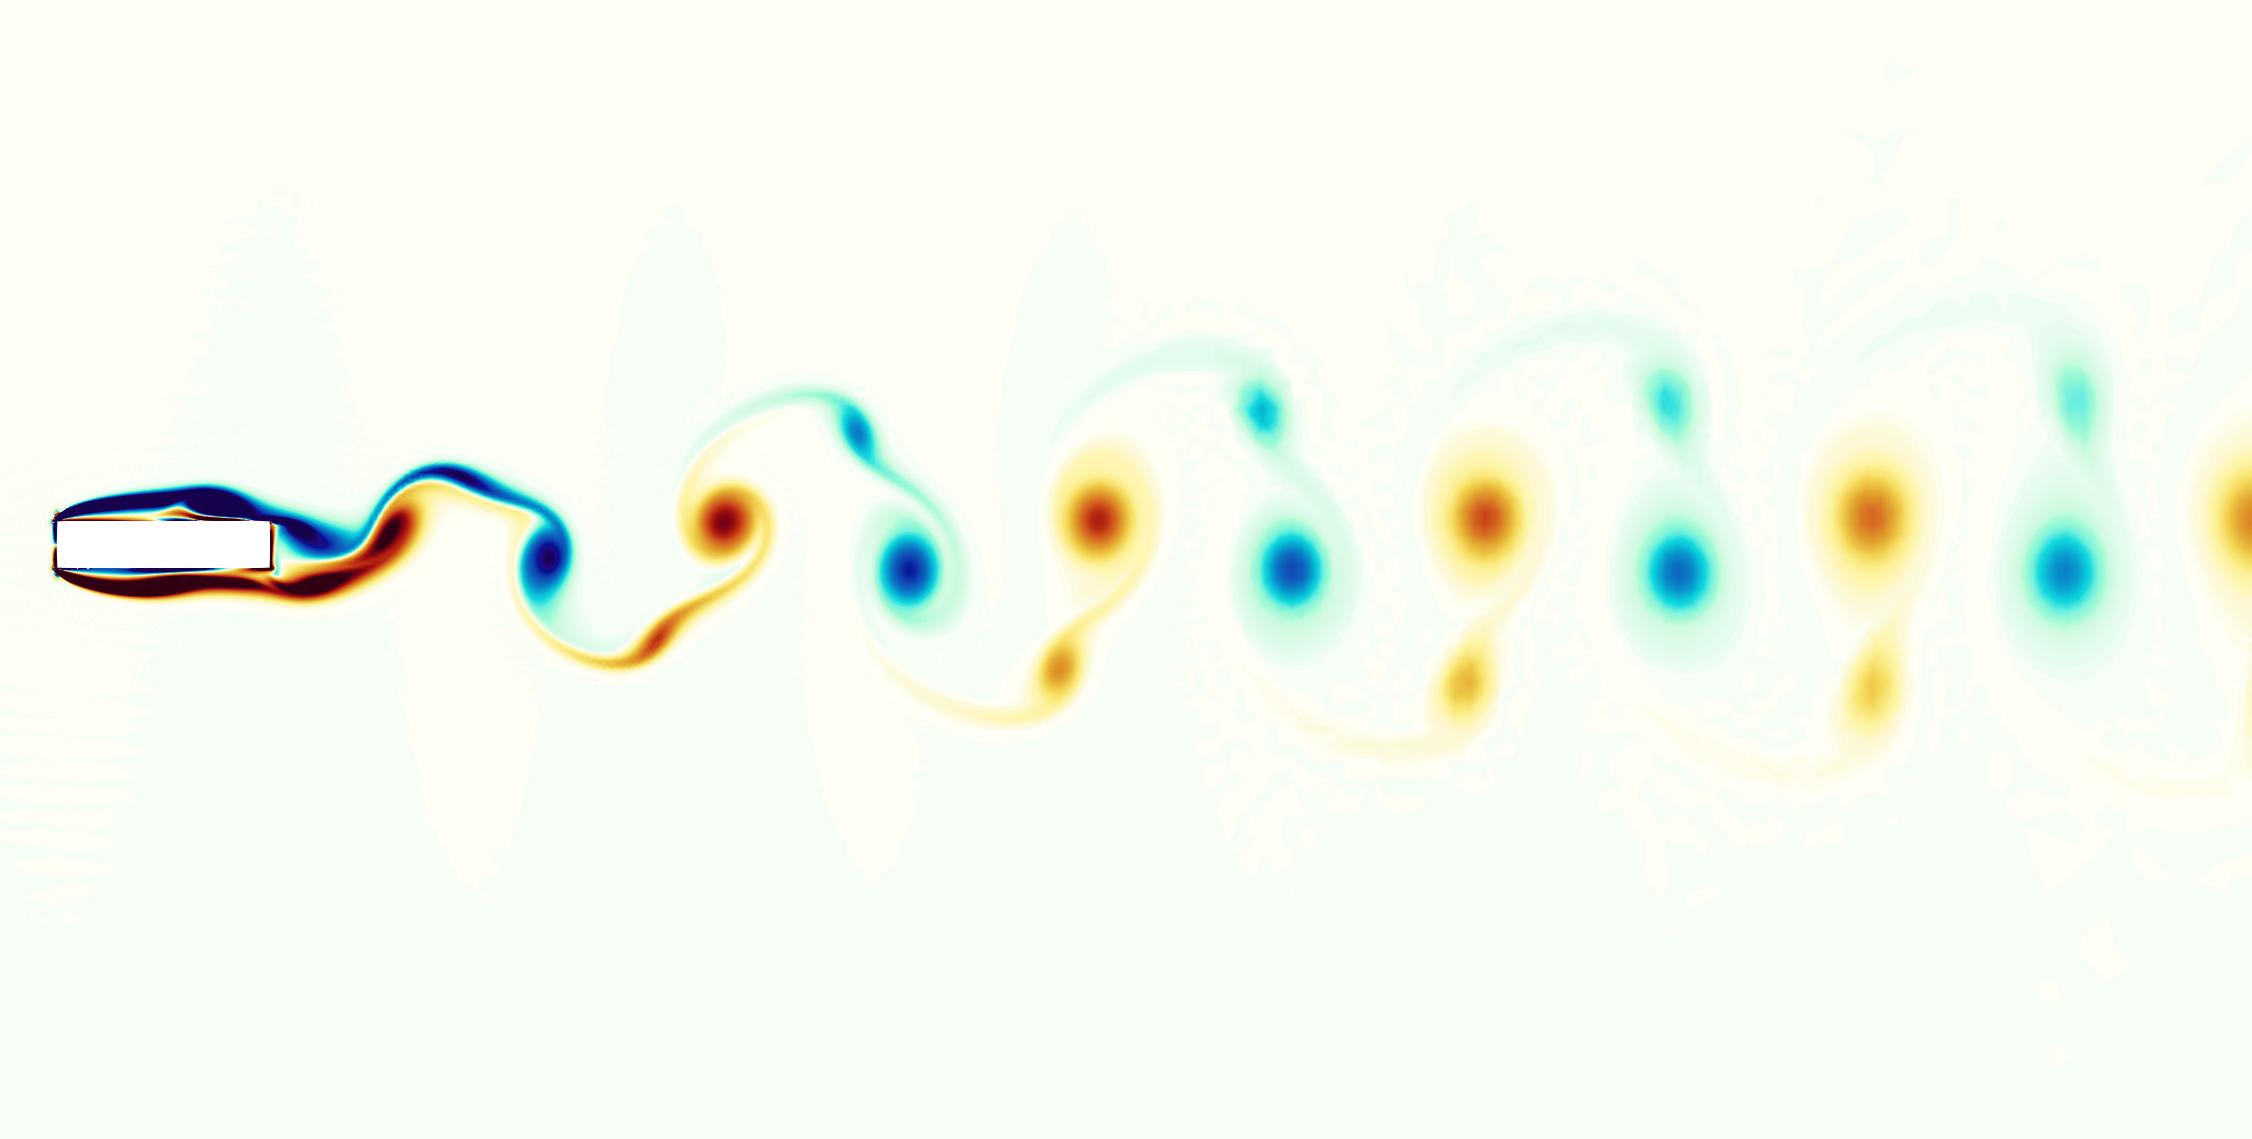
\includegraphics[trim={0 100 0 100},clip,width=0.49\textwidth]{./fig/AR4p5/vort_Re430_25.png}
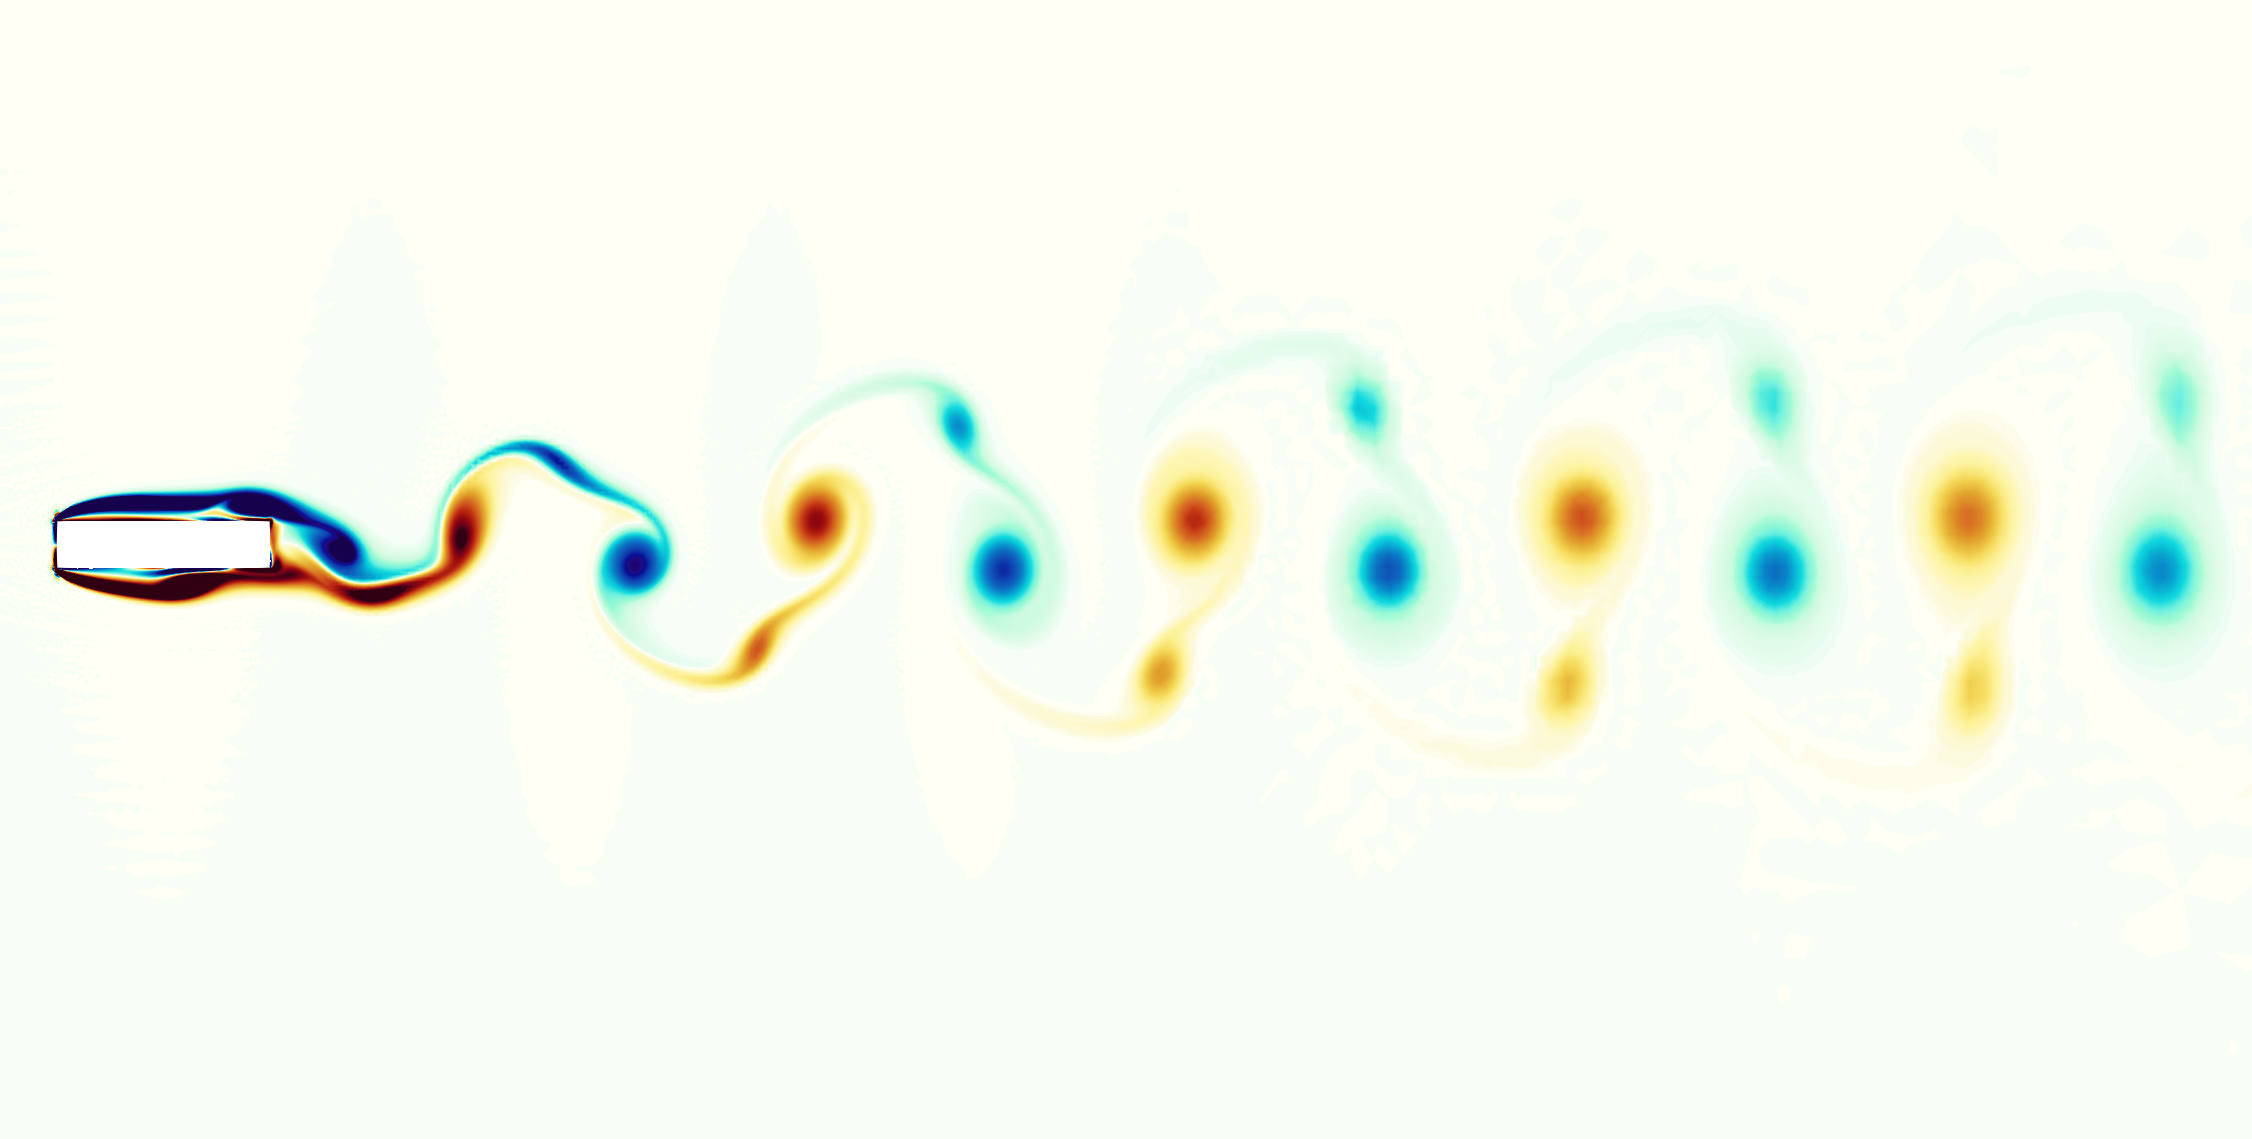
\includegraphics[trim={0 100 0 100},clip,width=0.49\textwidth]{./fig/AR4p5/vort_Re430_50.png}
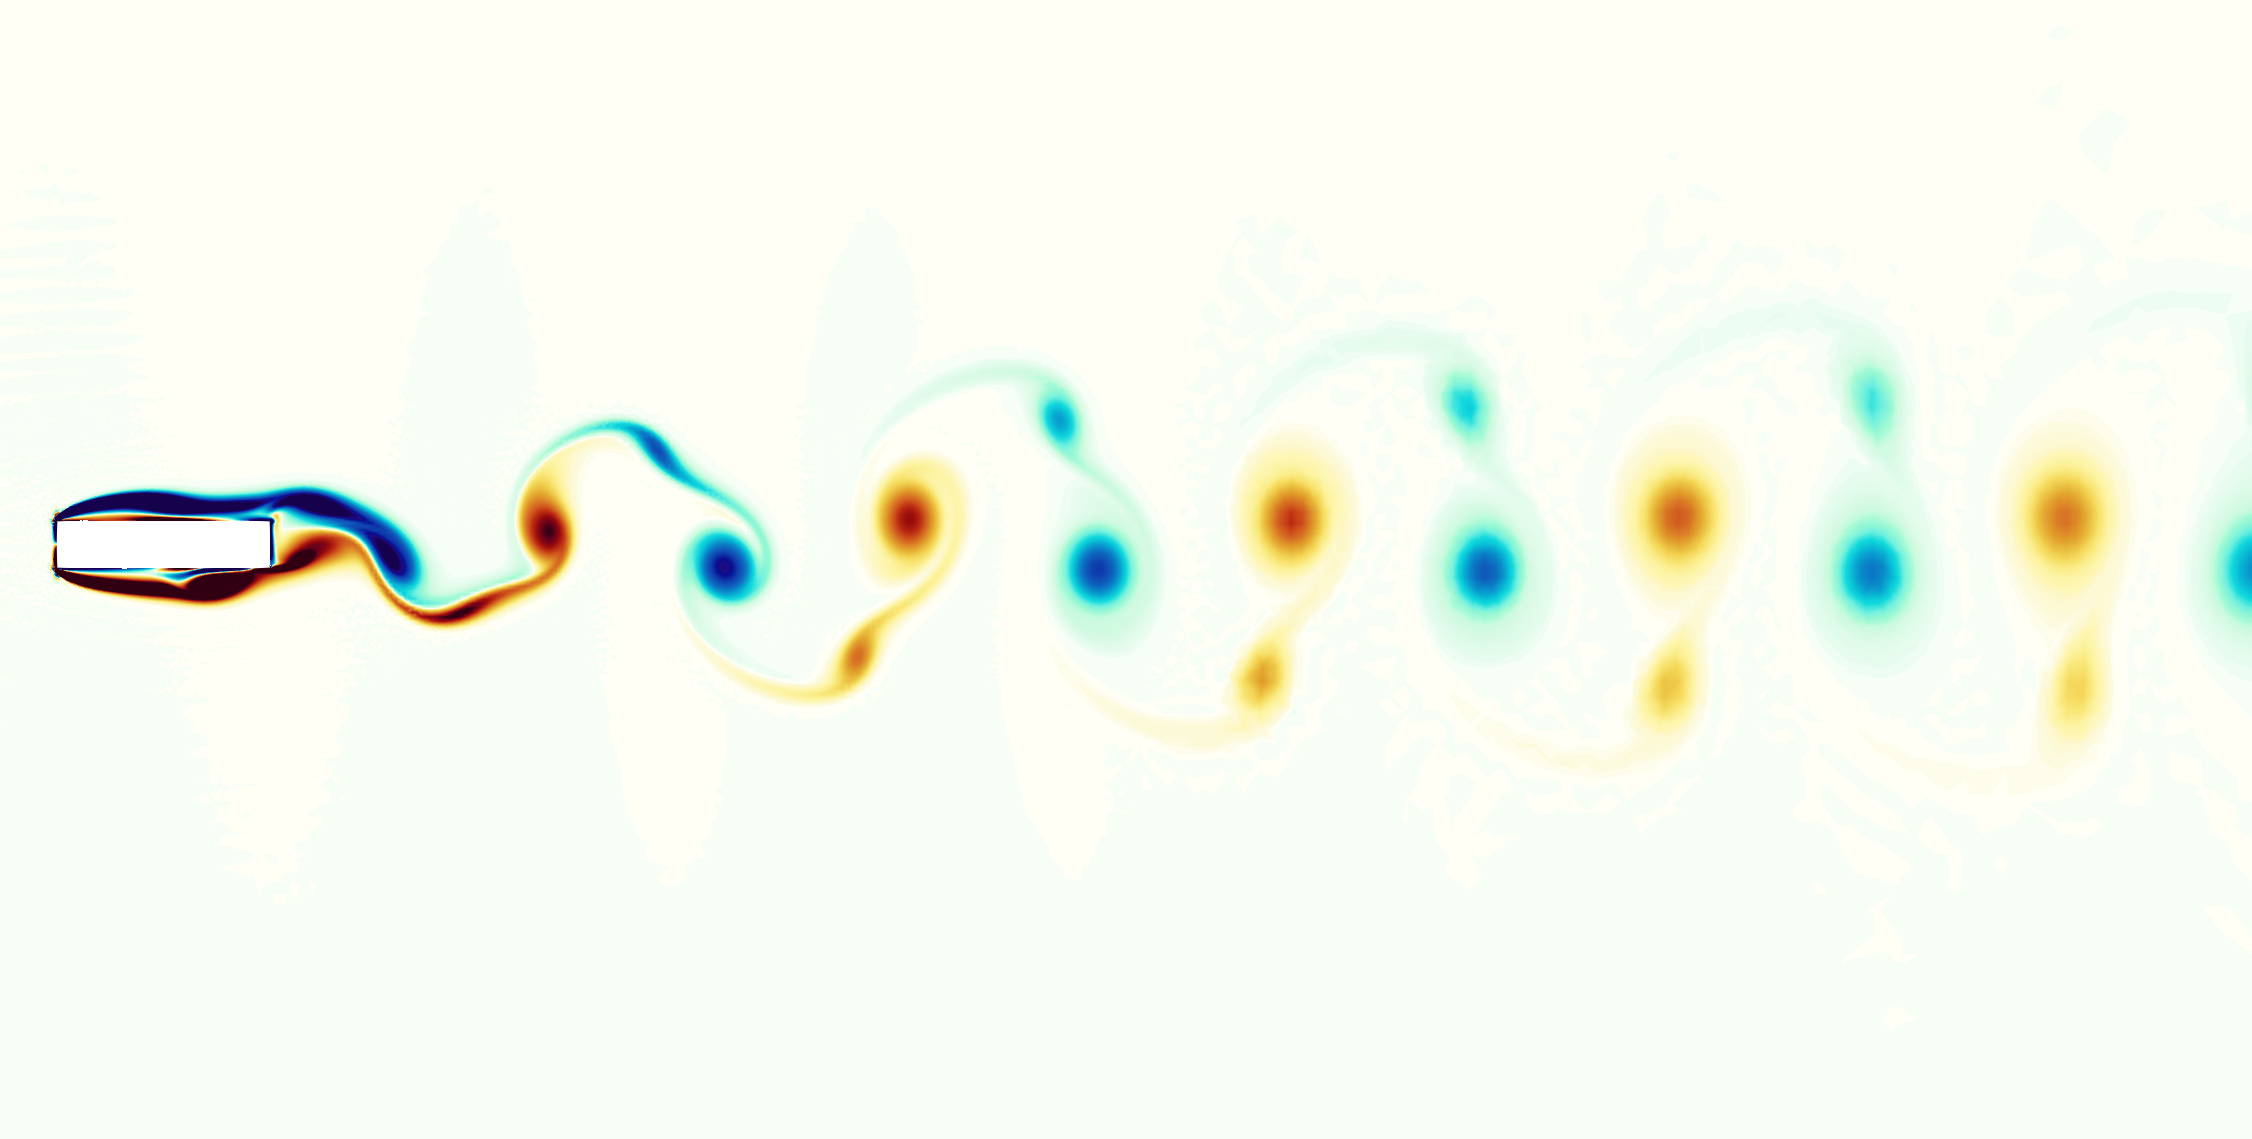
\includegraphics[trim={0 100 0 100},clip,width=0.49\textwidth]{./fig/AR4p5/vort_Re430_75.png}
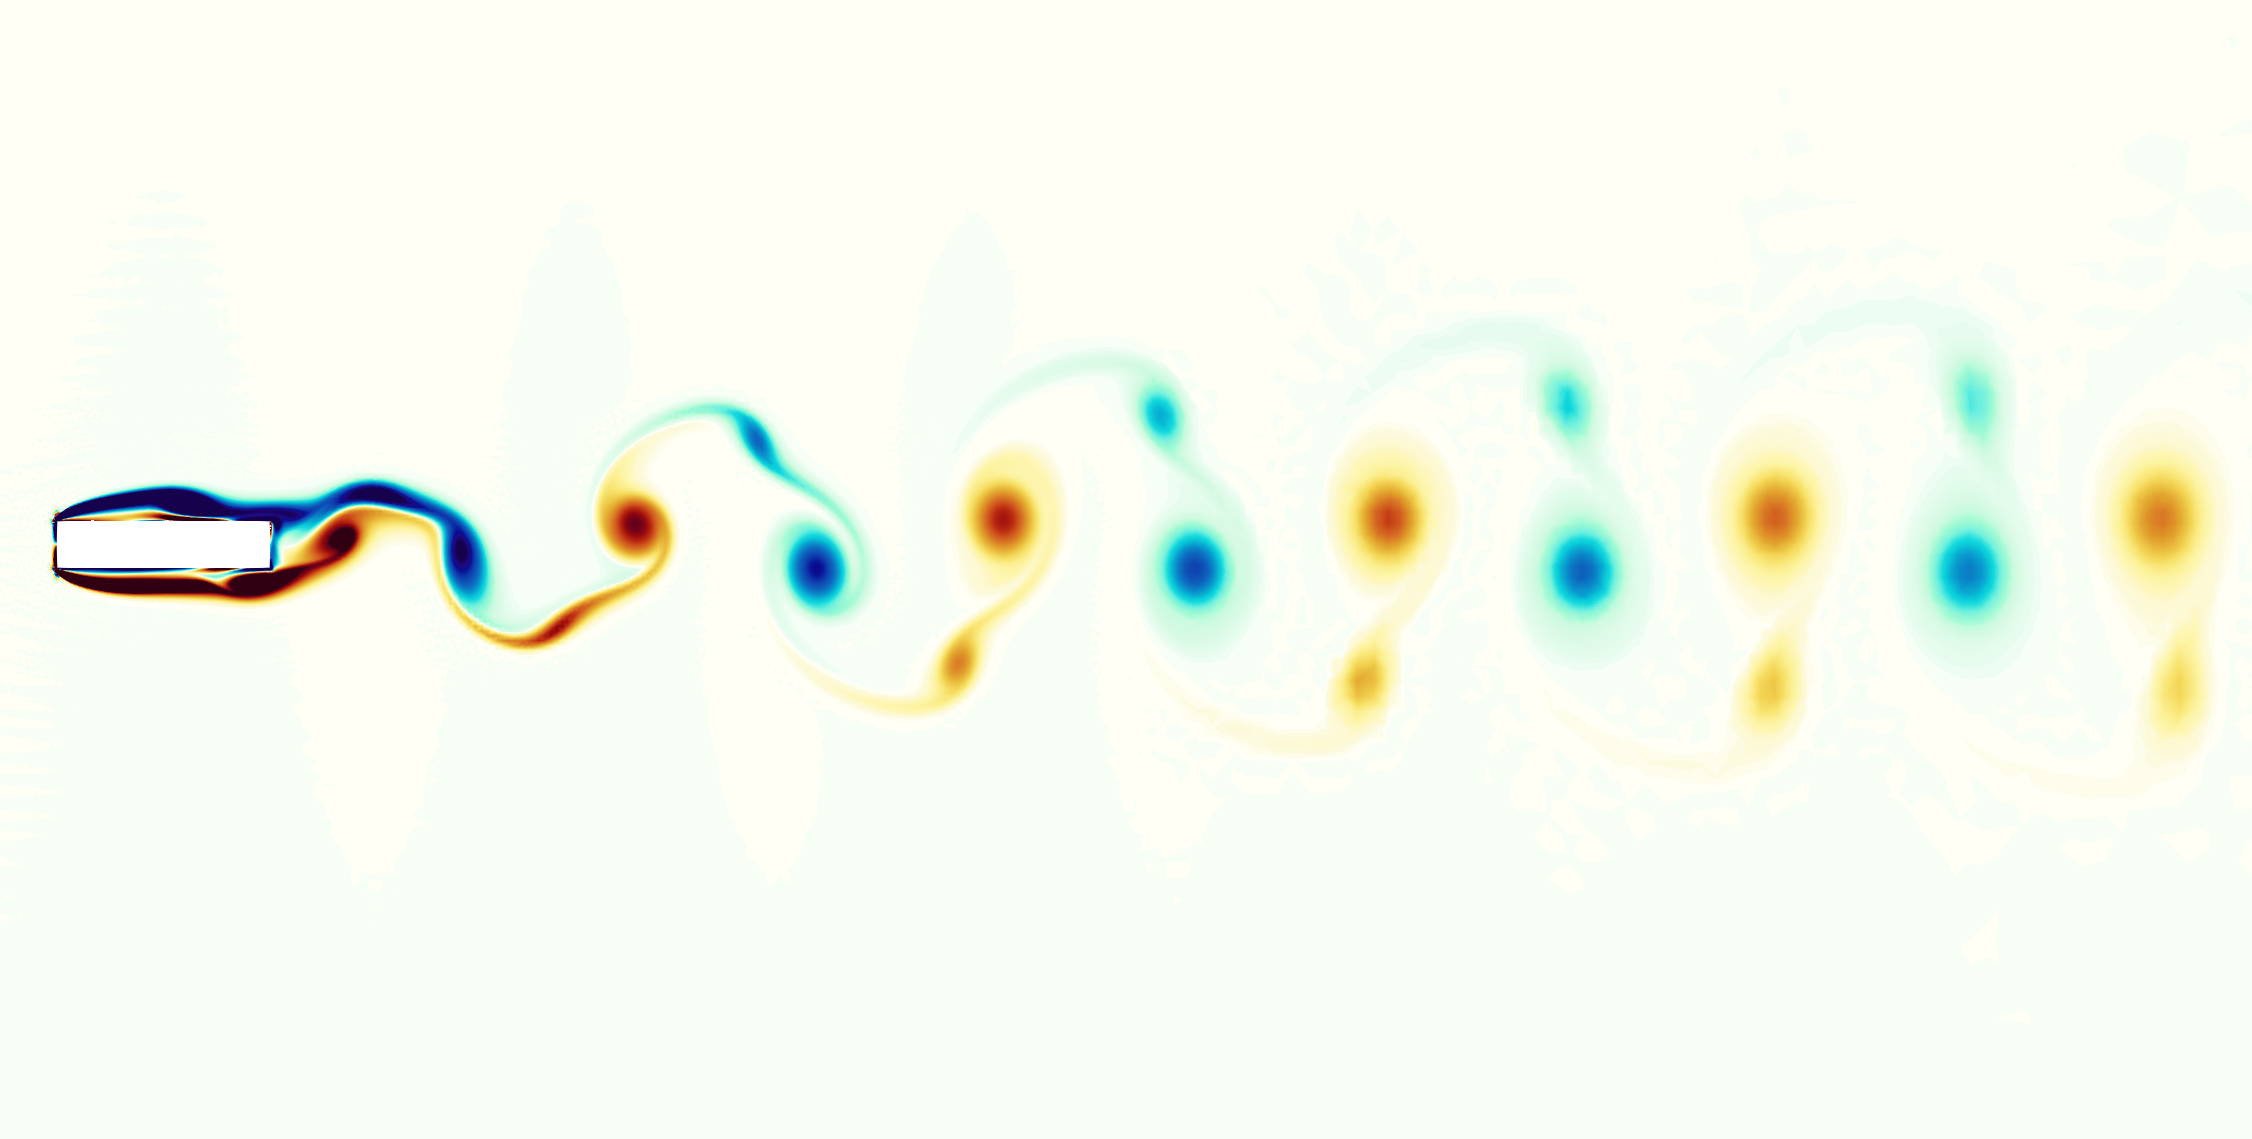
\includegraphics[trim={0 100 0 100},clip,width=0.49\textwidth]{./fig/AR4p5/vort_Re430_100.png}
\vspace{0.1cm}
\begin{tikzpicture}
\draw (-10,2) -- (8,2);
\end{tikzpicture}
\vspace{0.1cm}
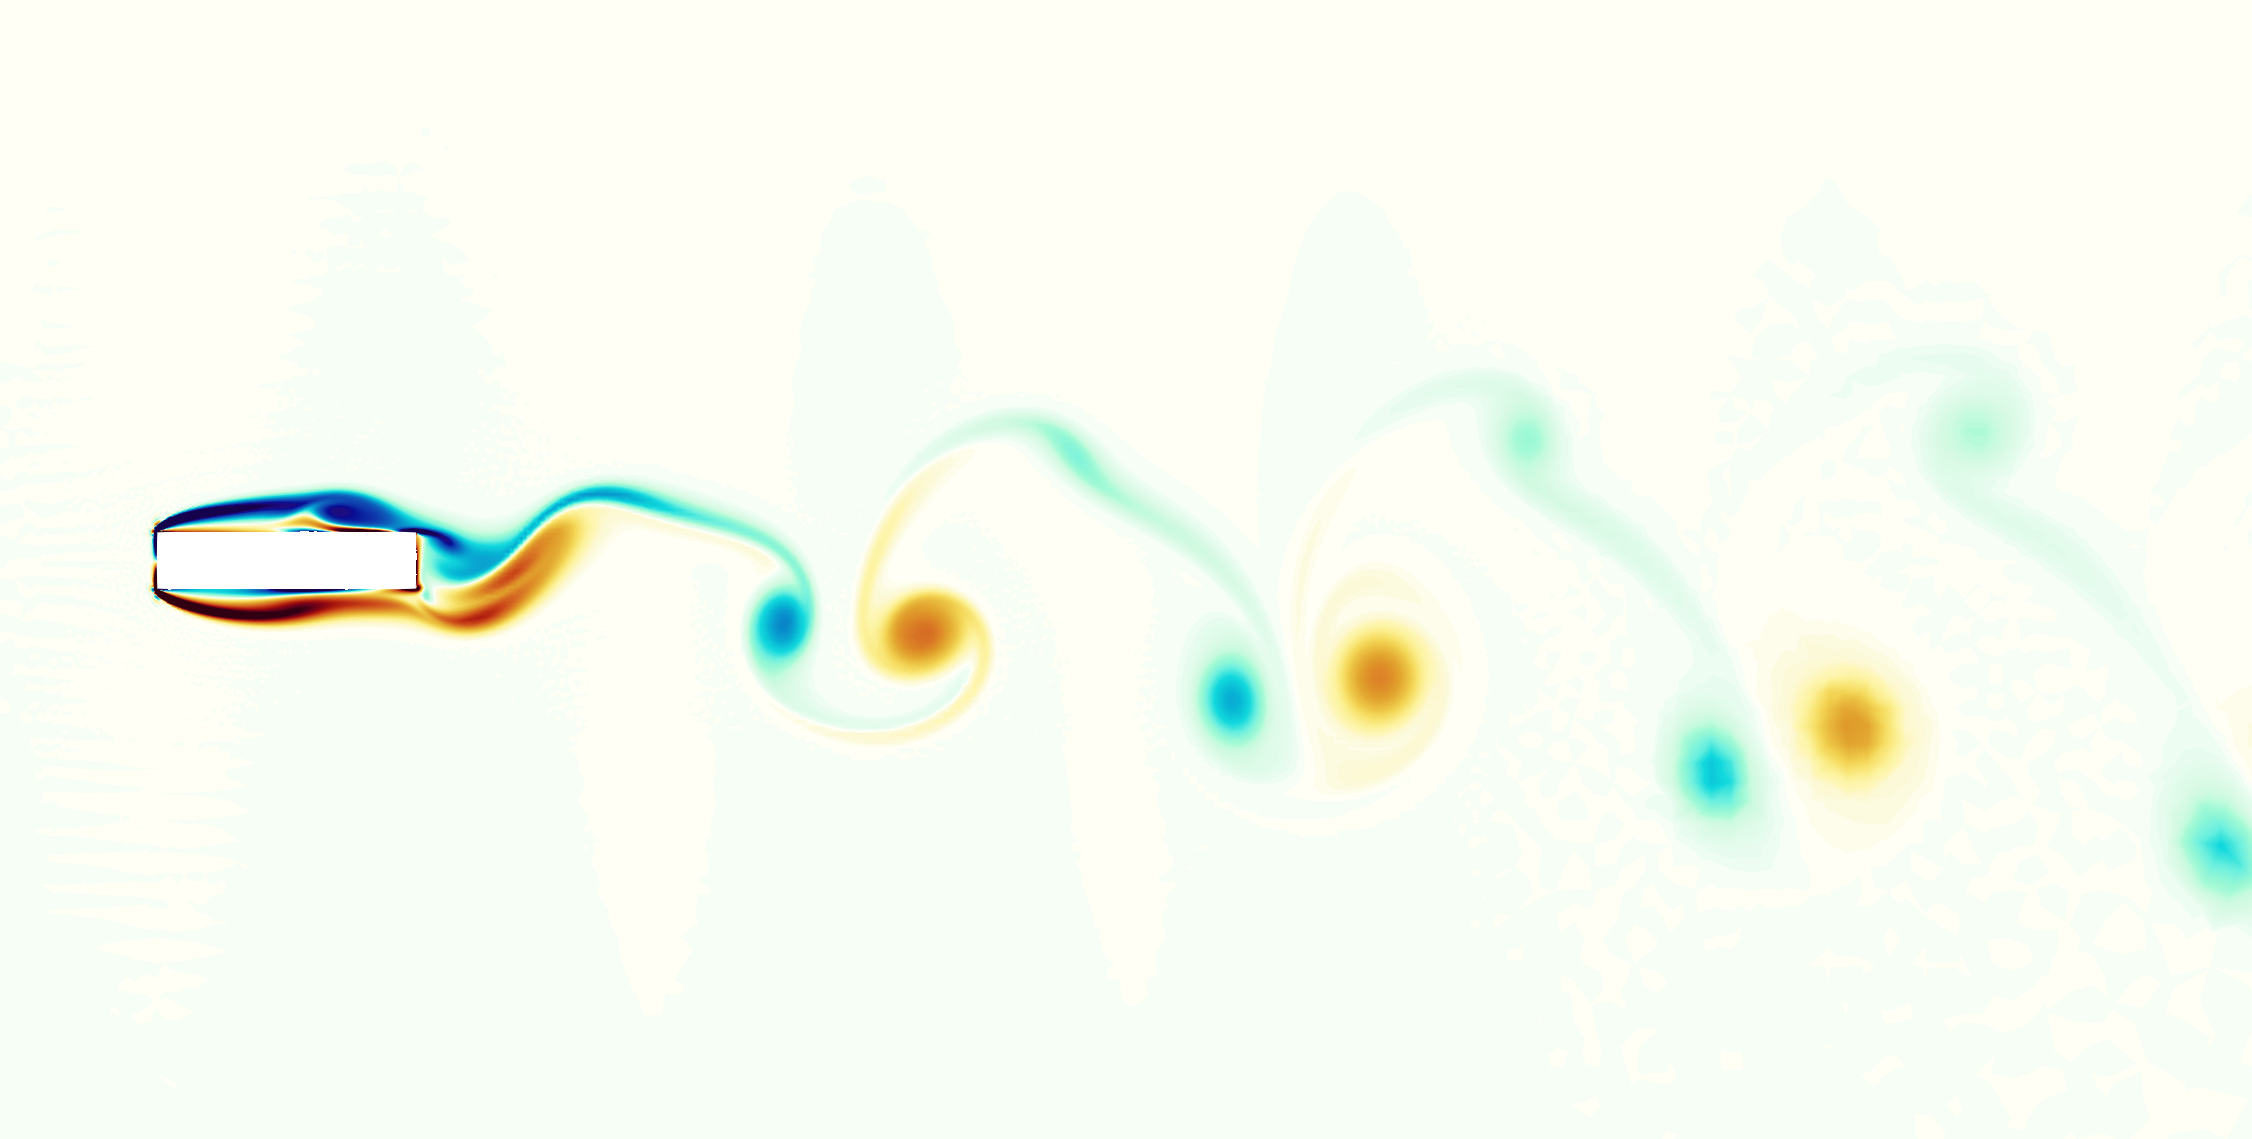
\includegraphics[trim={0 100 0 100},clip,width=0.49\textwidth]{./fig/AR4p5/vort_Re450_25.png}
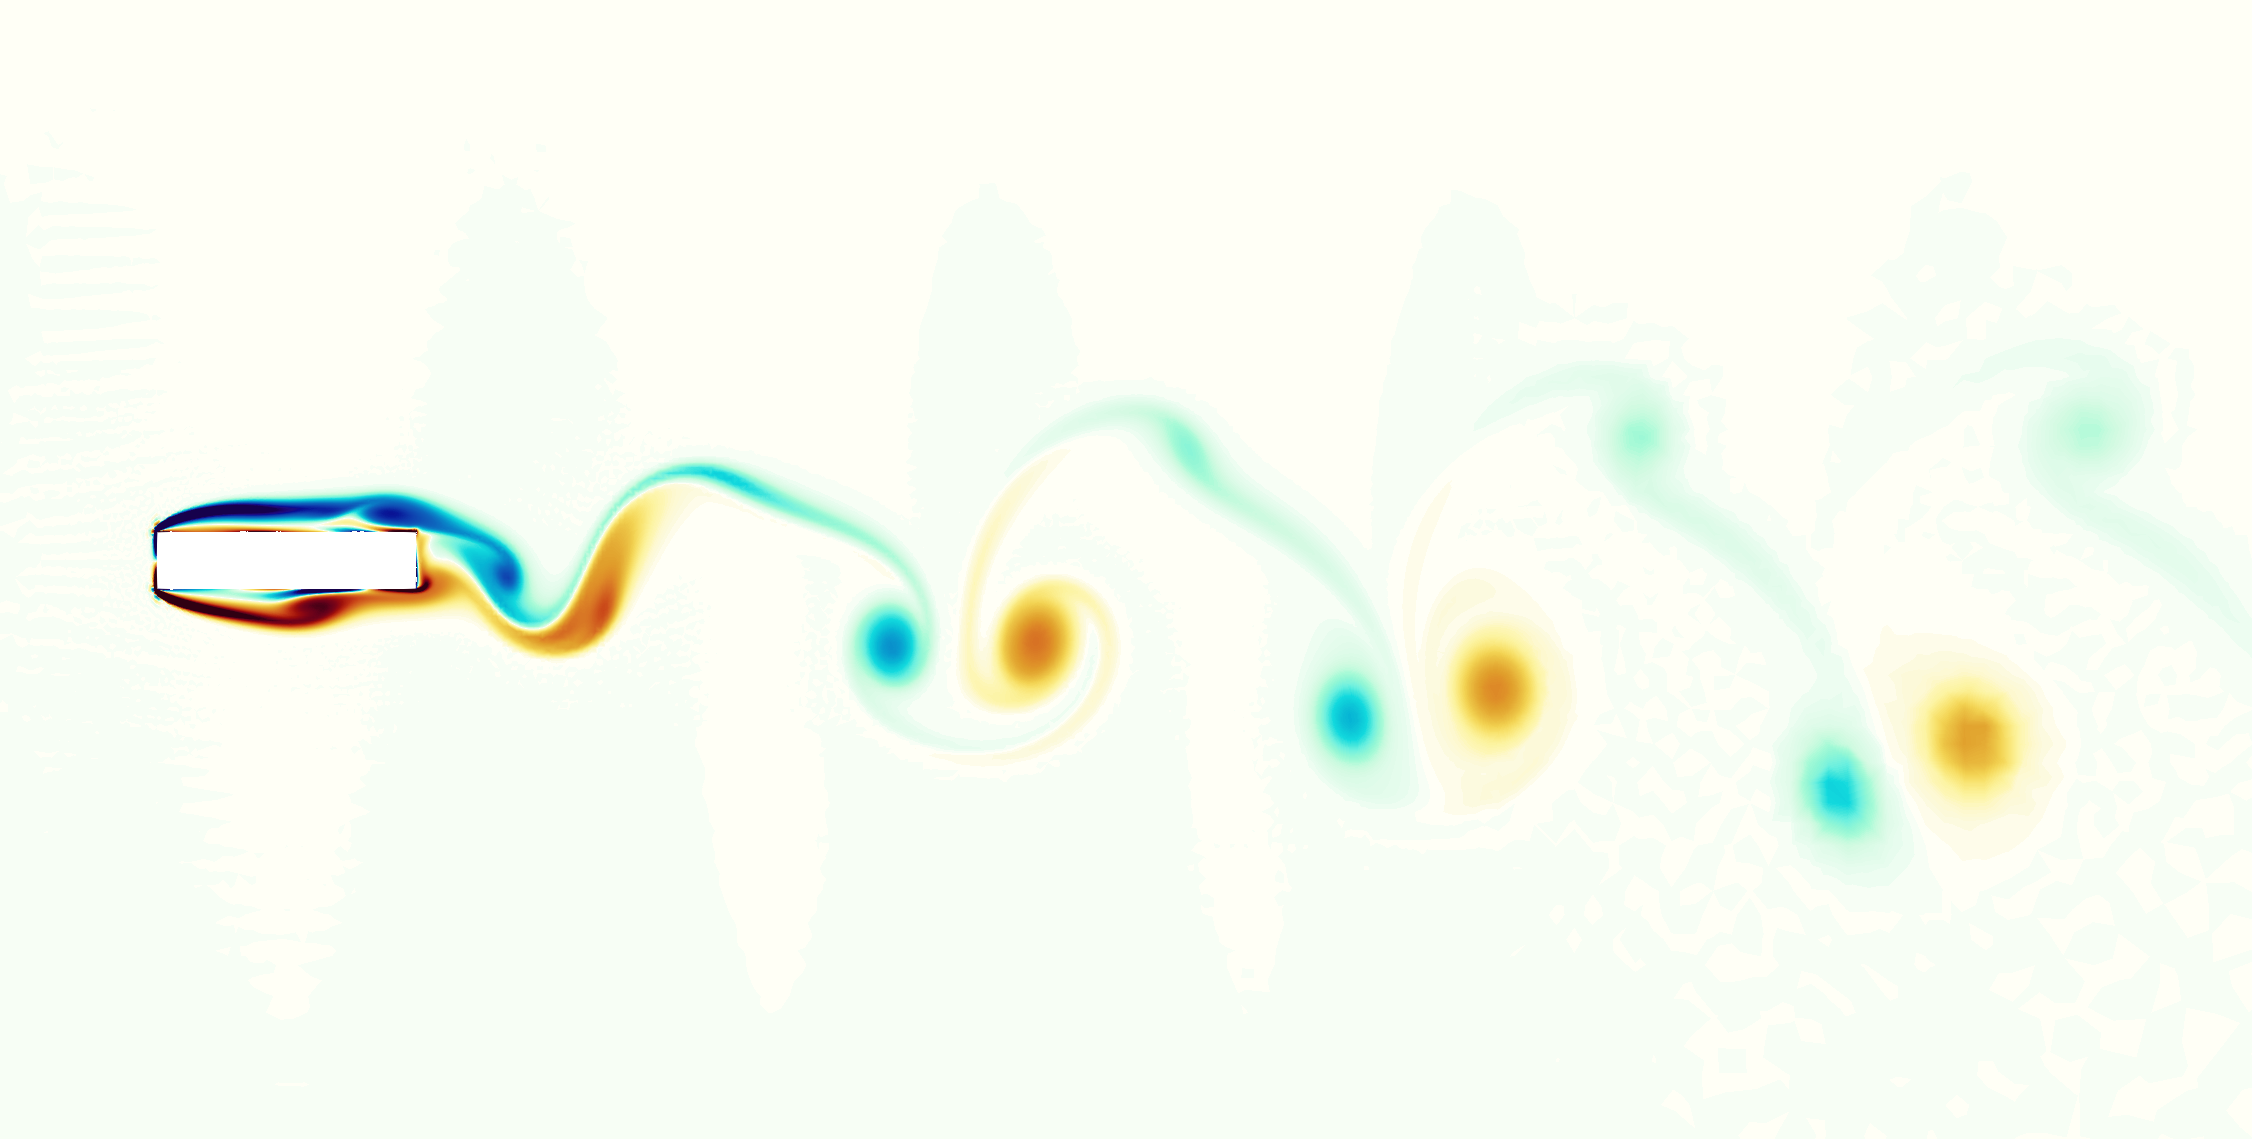
\includegraphics[trim={0 100 0 100},clip,width=0.49\textwidth]{./fig/AR4p5/vort_Re450_50.png}
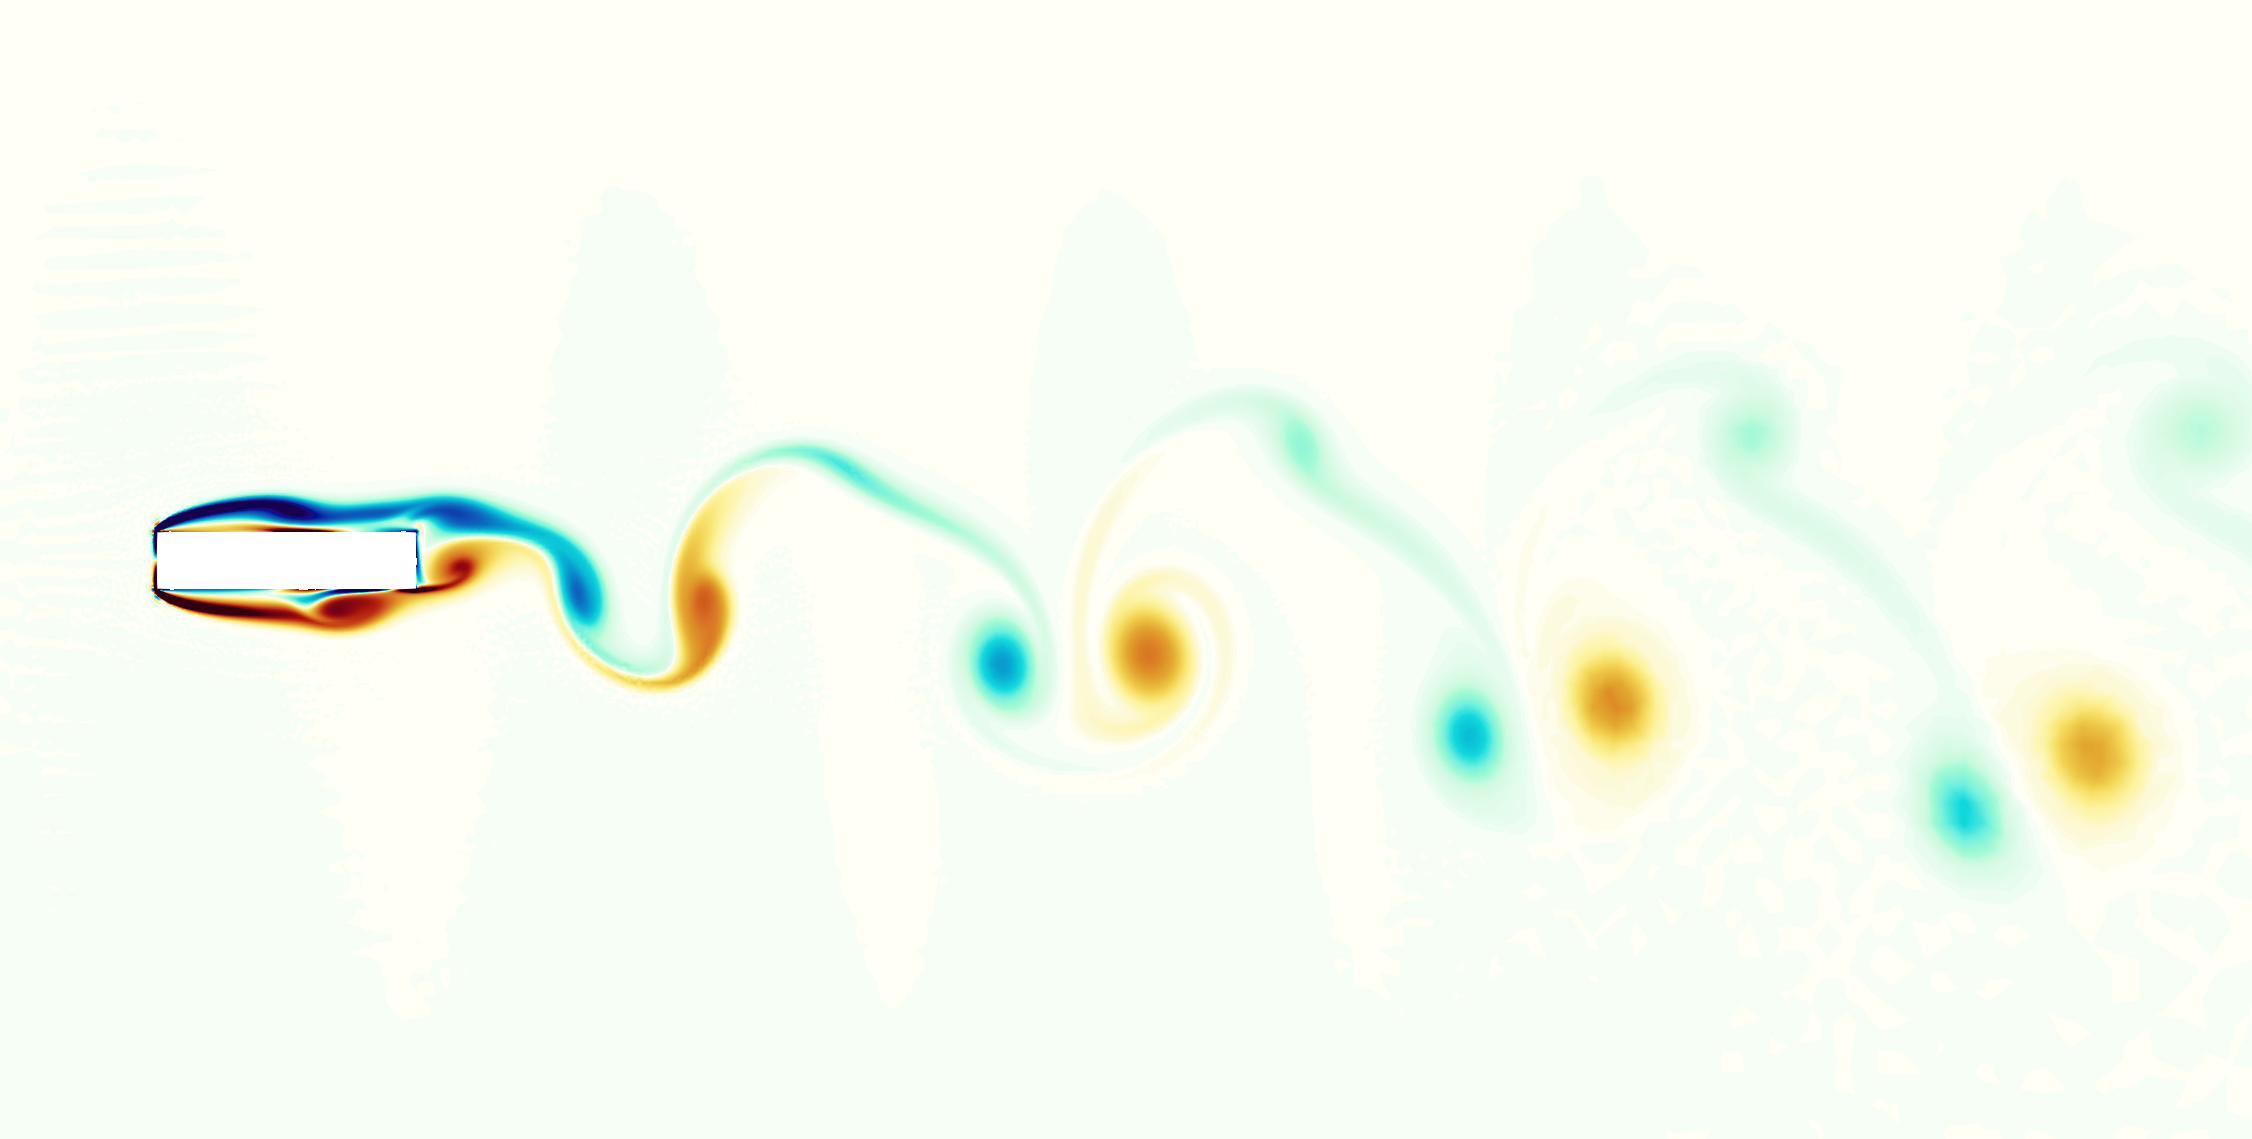
\includegraphics[trim={0 100 0 100},clip,width=0.49\textwidth]{./fig/AR4p5/vort_Re450_75.png}
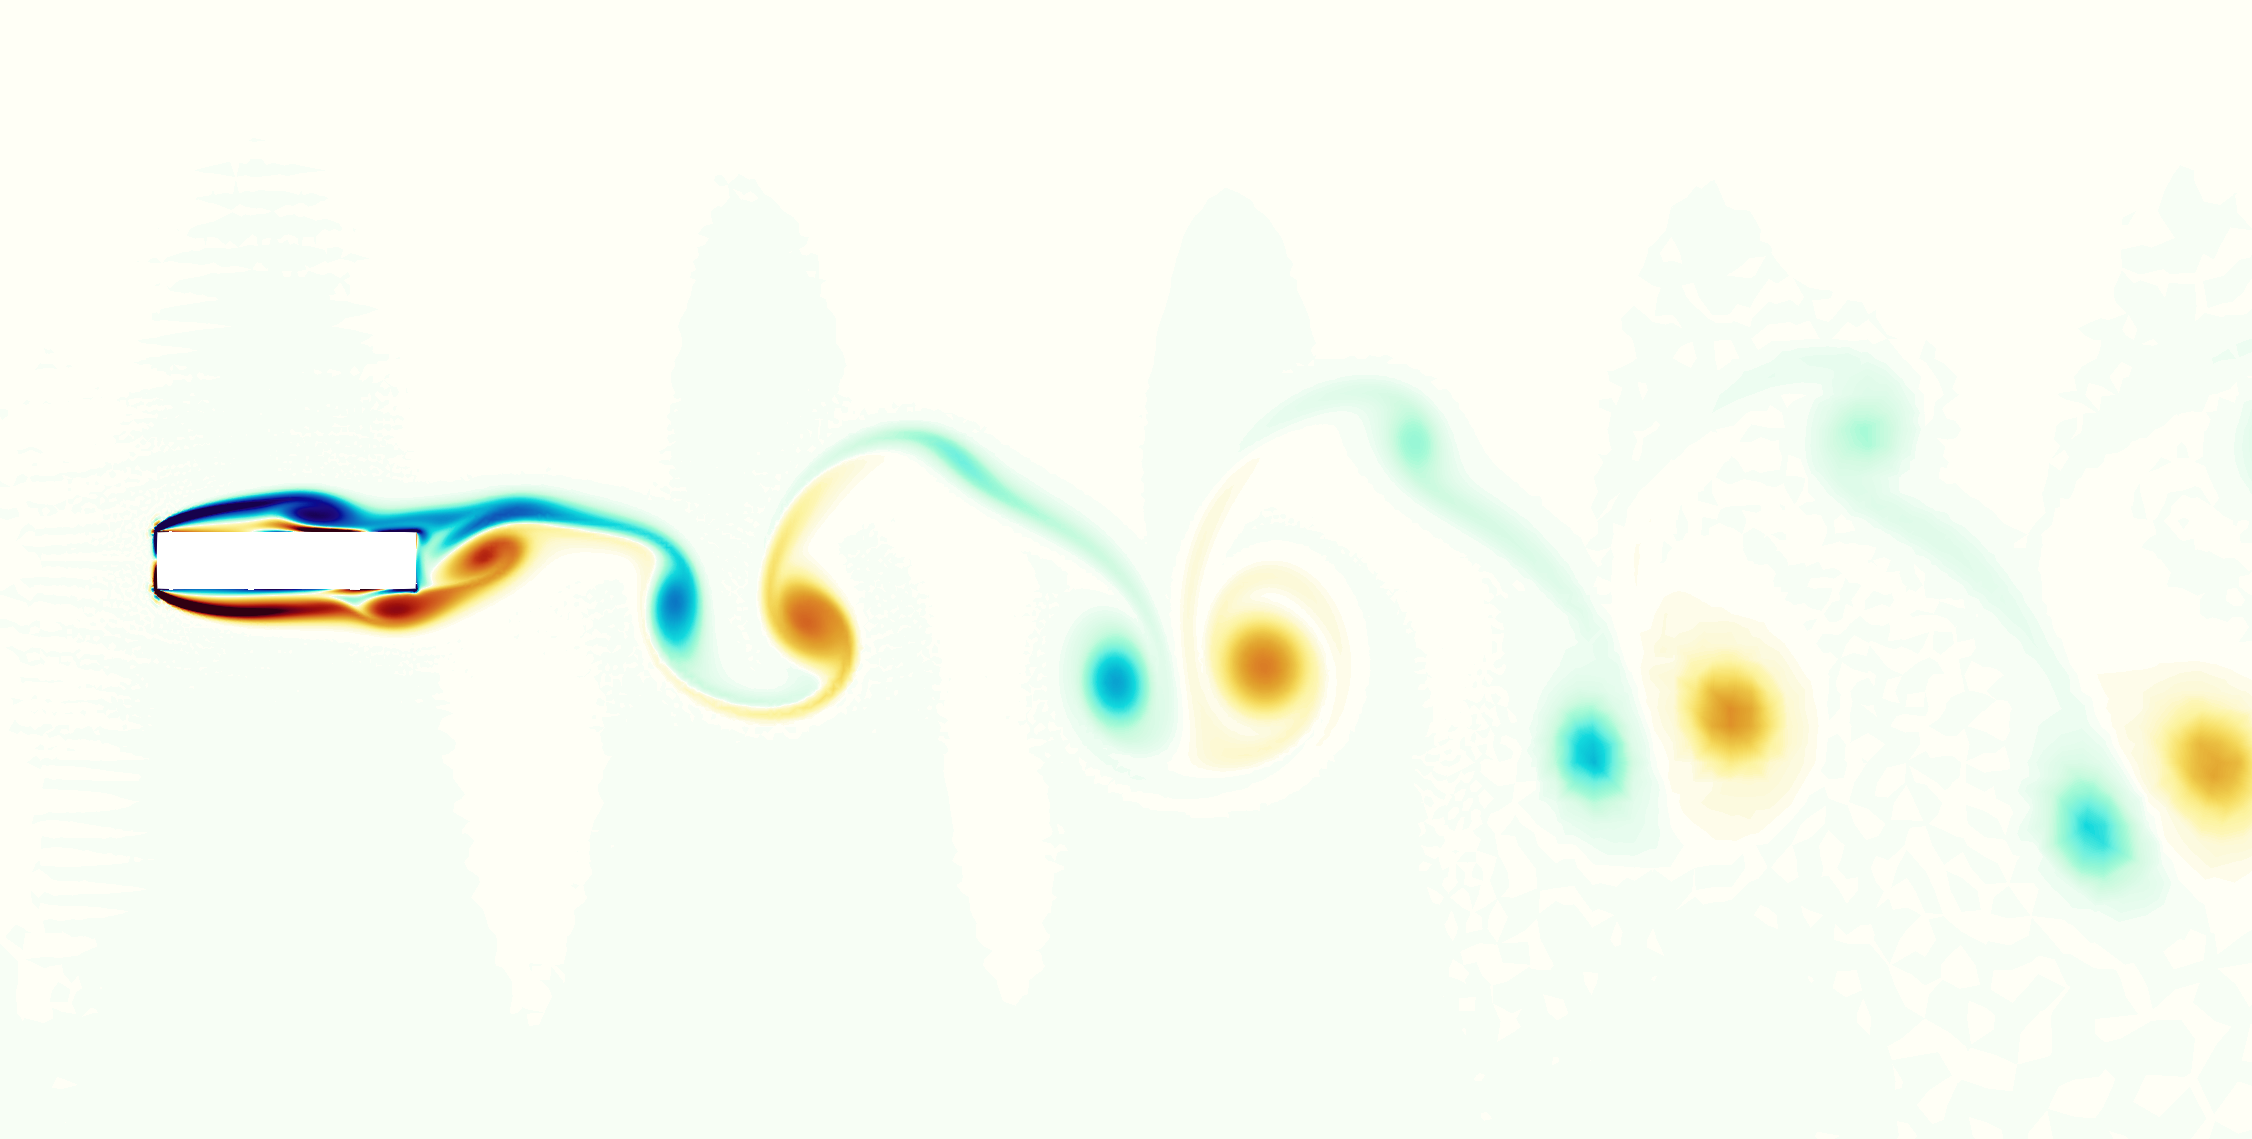
\includegraphics[trim={0 100 0 100},clip,width=0.49\textwidth]{./fig/AR4p5/vort_Re450_100.png}
\caption{Top: Evolution of the vorticity in one oscillation period for $\AR=4.5$ and $Re=430$. Bottom: Evolution of the vorticity in one oscillation period for $\AR=4.5$ and $Re=450$.}
\label{fig:vort_AR4p5_Re450}
\end{figure}

\begin{figure}
\centering
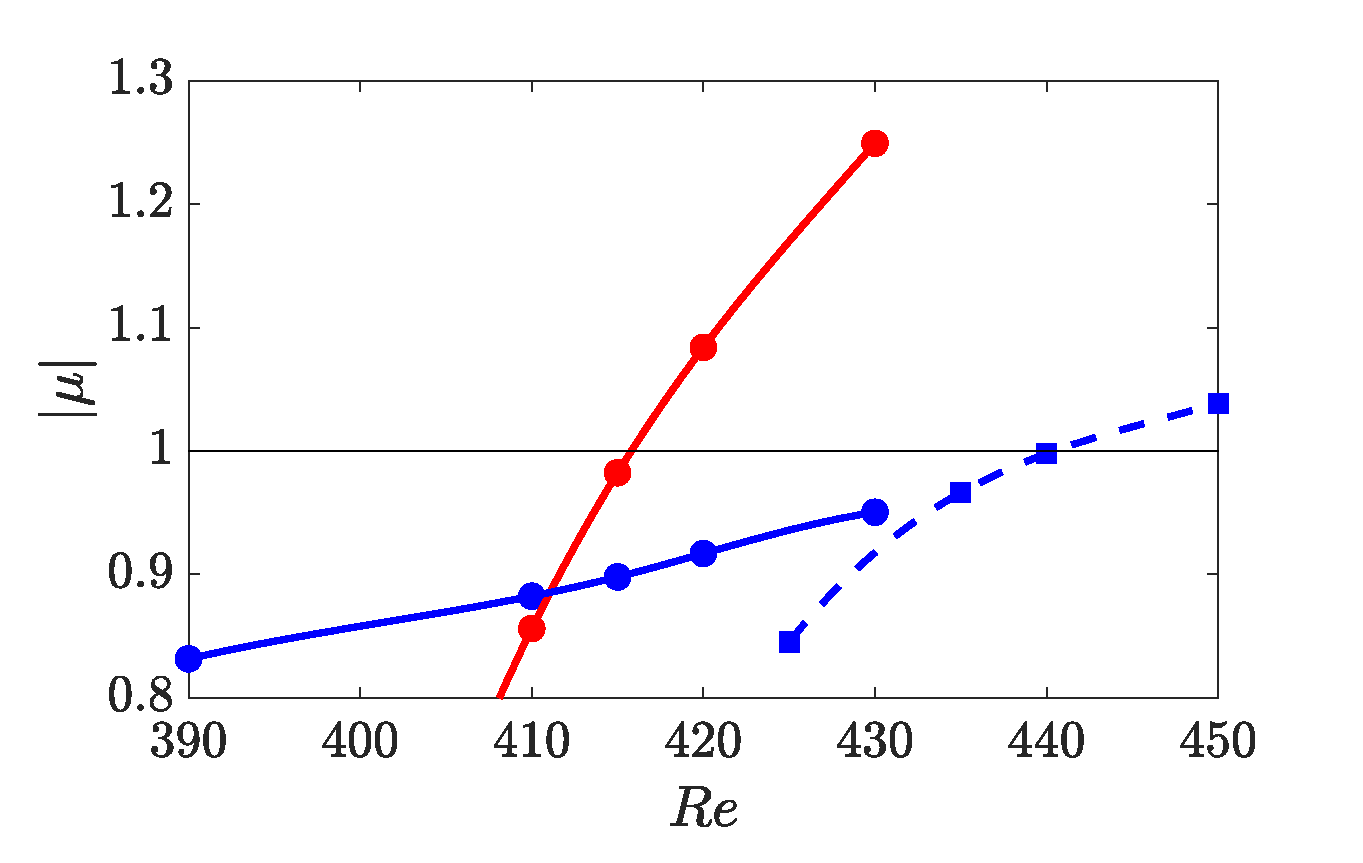
\includegraphics[width=0.49\textwidth]{./fig/AR4p5/multipliers_2D.eps}
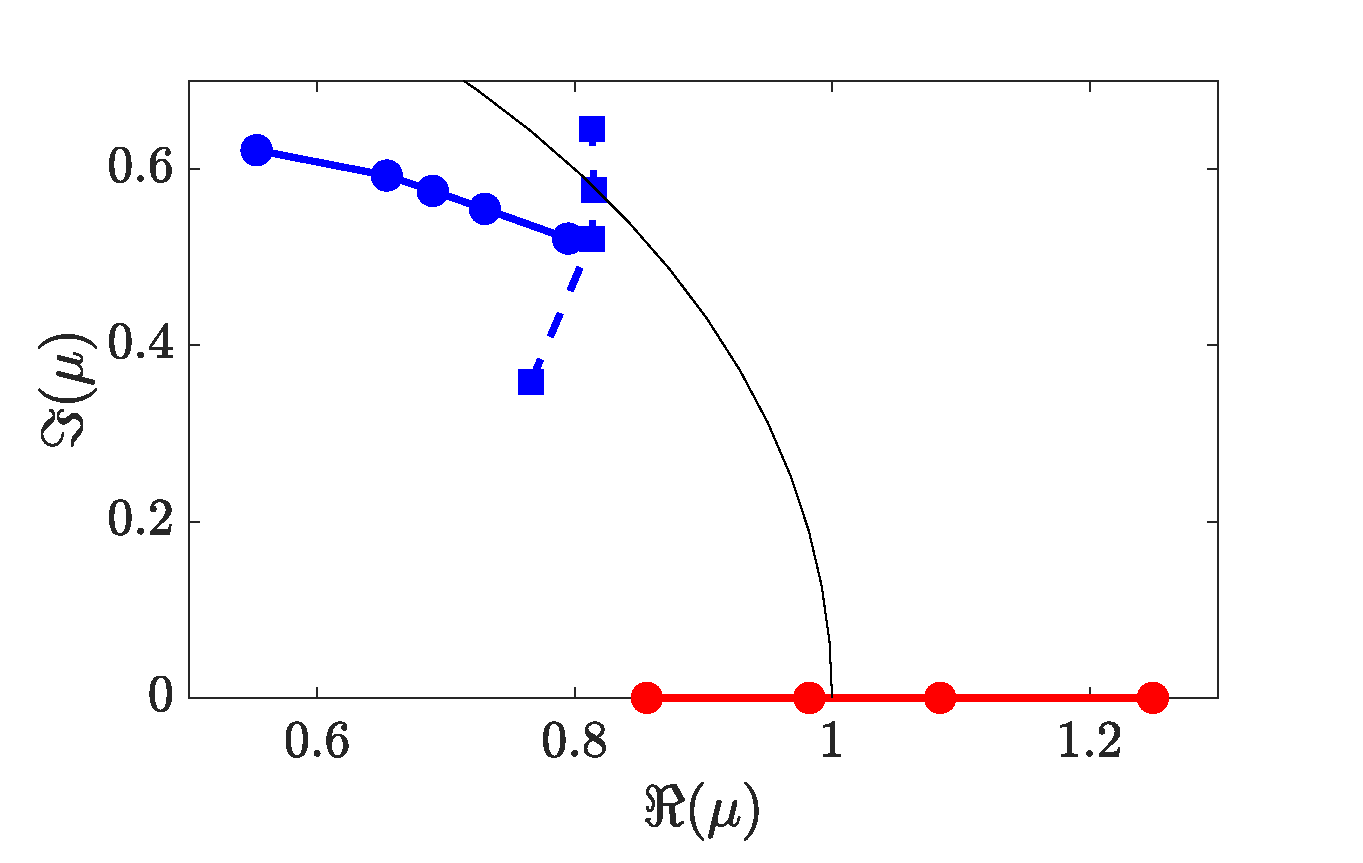
\includegraphics[width=0.49\textwidth]{./fig/AR4p5/multipliers_2D_b.eps}
\vspace{0.1cm}
\begin{tikzpicture}
\draw (-10,2) -- (8,2);
\end{tikzpicture}
\vspace{0.1cm}
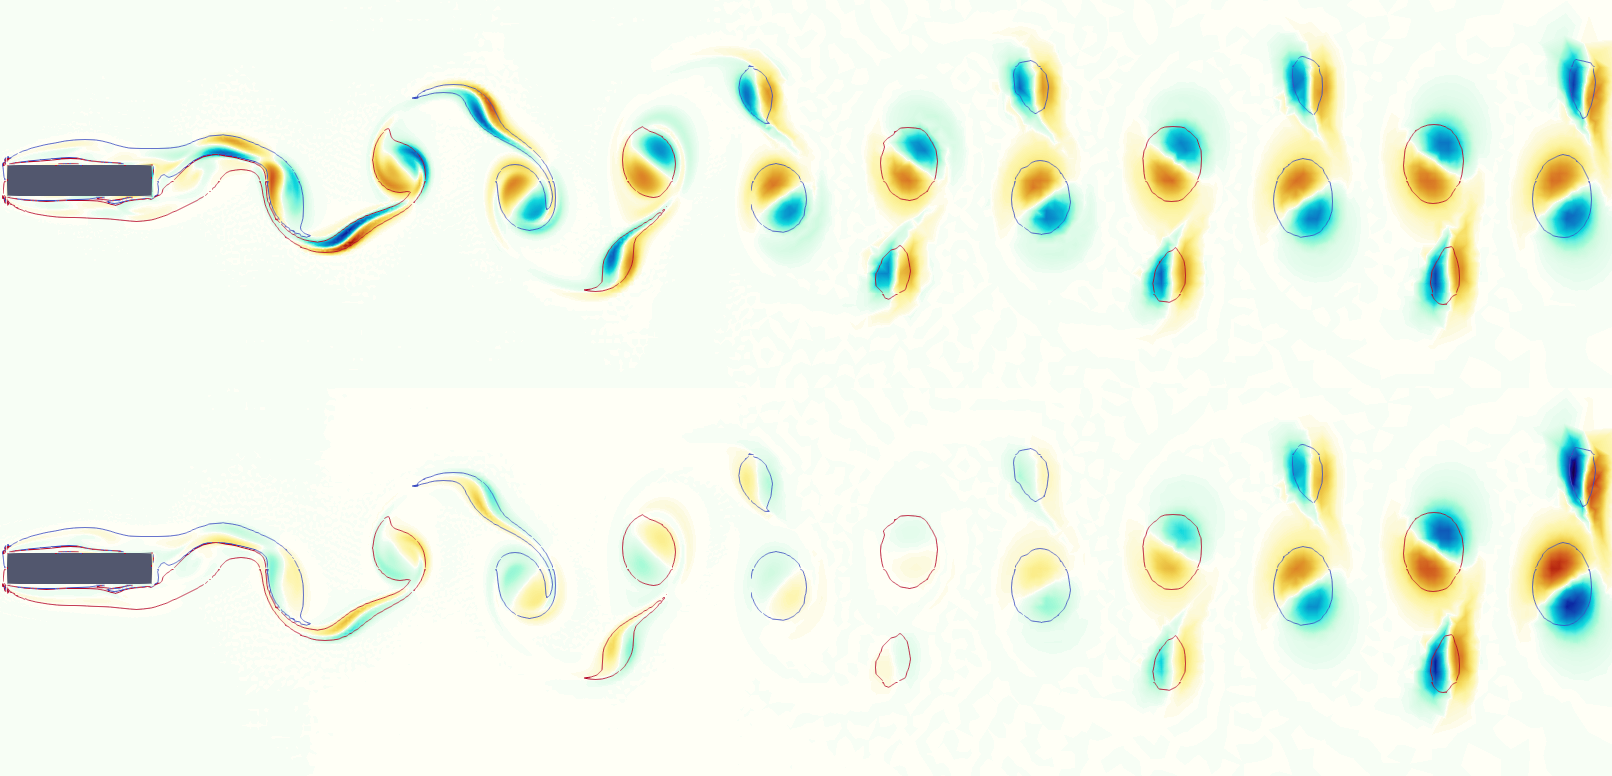
\includegraphics[width=0.7\textwidth]{./fig/AR4p5/omegaz_beta0_Re430_AB.png}
\vspace{0.1cm}
\begin{tikzpicture}
\draw (-10,2) -- (8,2);
\end{tikzpicture}
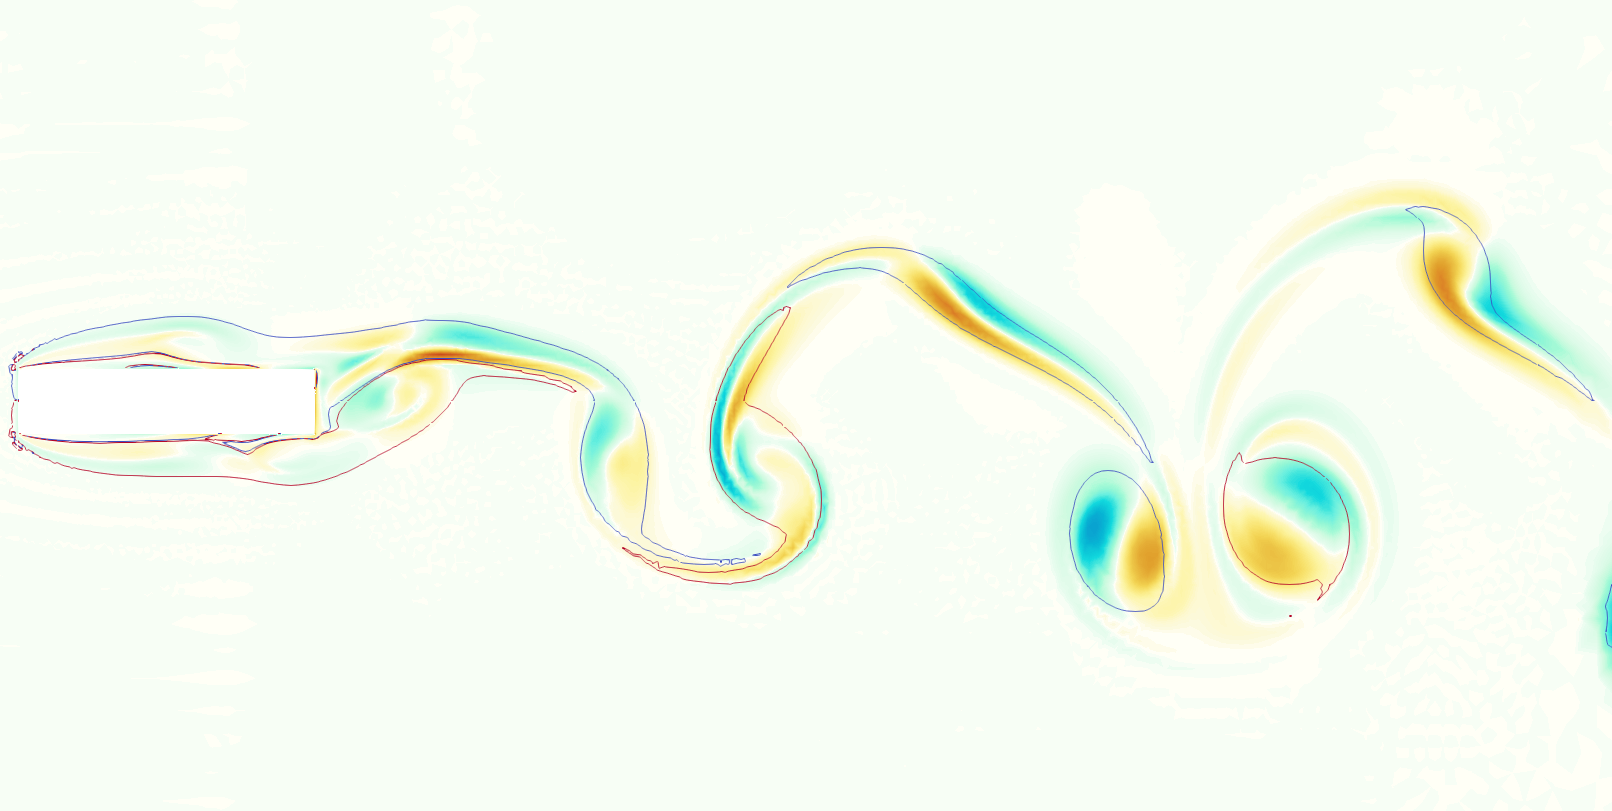
\includegraphics[width=0.7\textwidth]{./fig/AR4p5/Floqetmode_beta_0_Re450_AR4p5.png}
\caption{$2D$ bifurcation of the periodic flow past a rectangular cylinder with $\AR=4.5$. Top: Multipliers associated with the straight (solid) and slanted (dashed) wake for $\AR=4.5$. The left panel plots $|\mu|$ as a function of $\beta$. The red colour refers to real and positive multipliers, while the blue colour refer to complex mutlpliers. The right panel shows the dependence of $\Re(\mu)$ and $\Im(\mu)$ on $Re$. Note that the slanted wake is the results of the synchronous instability described by the red branch. Once the wake becomes slanted a new branch with complex conjugate multipliers arises that becomes unstable at $Re \approx 450$. Centre: Floquet modes associated with the straight wake; the colours are for the spanwise vorticity and the above and bottom panel refer to the red and blue branches respectively. Bottom: Floquet mode associated with the blue branch of the slanted wake.}
\label{fig:AR4p5_modes_Re430_beta0}
\end{figure}

\begin{figure}
  \centering
  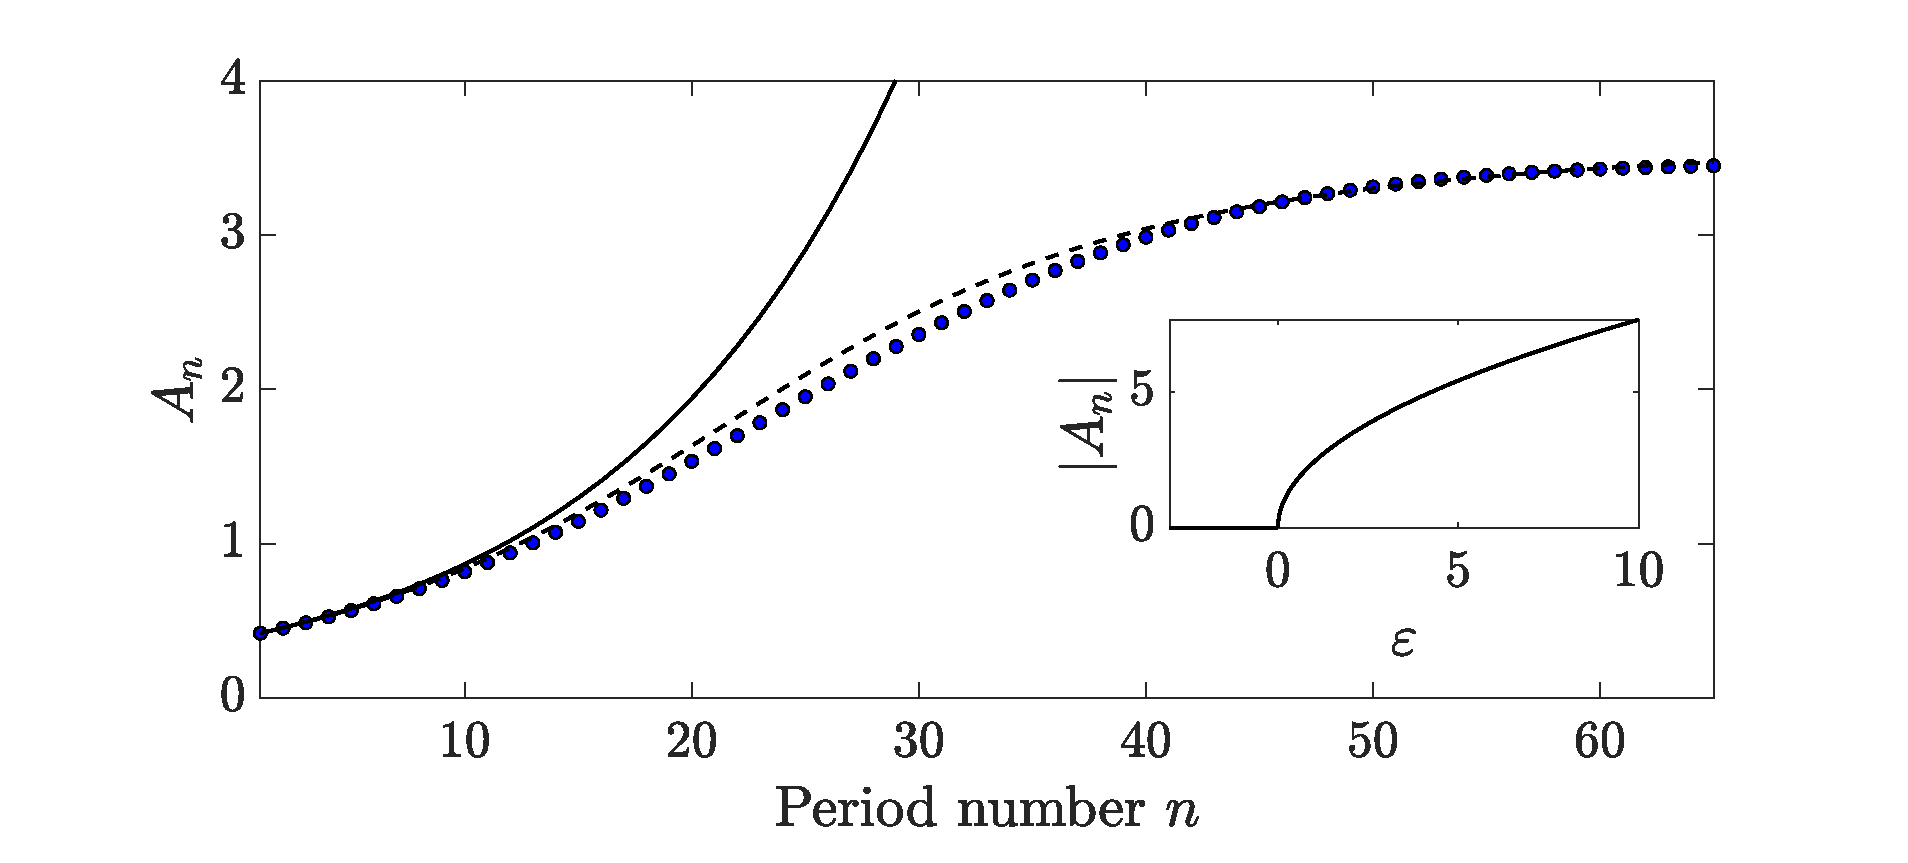
\includegraphics[width=0.7\textwidth]{./fig/AR4p5/Nlgrowth_Re420.eps}
  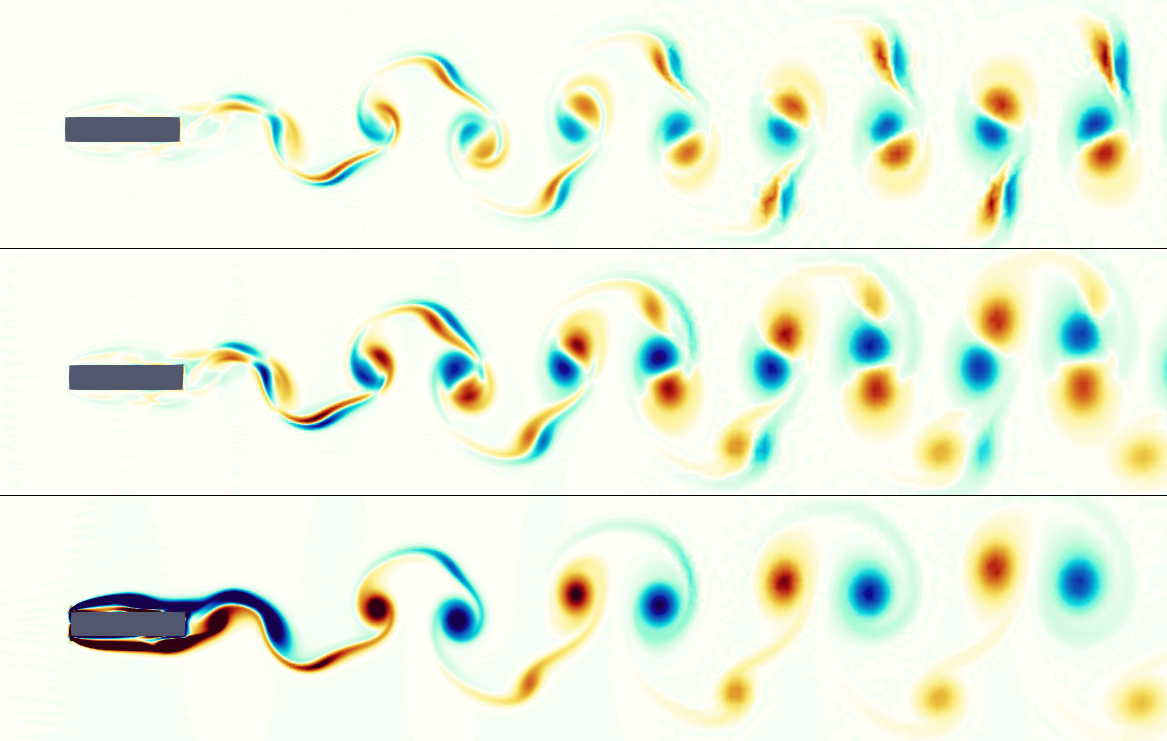
\includegraphics[width=0.8\textwidth]{./fig/AR4p5/LinNonLin_Re420.png}
  \caption{Nonlinear growth of the 2D perturbation to the wake near the secondary instability threshold for $\AR=4.5$ and $Re=420$. Top: the blue circles are the amplitude of $A_n$ evaluated from simulations of the full Navier--Stokes equations at $Re=420$. The solid line shows the prediction $A_{n+1} = \mu A_n$, while the dashed line shows the prediction $A_{n+1} = ( \mu + \alpha_1 A_n + \alpha_2 A_n^3 ) A_n$, with $\alpha_1 = -0.01114$ and $\alpha_2 = 0.000359$. The inset shows the bifurcation diagram. Bottom: snapshots of the vorticity field for linear and nonlinear perturbations and of the total field.}
\end{figure}

\begin{figure}
\centering
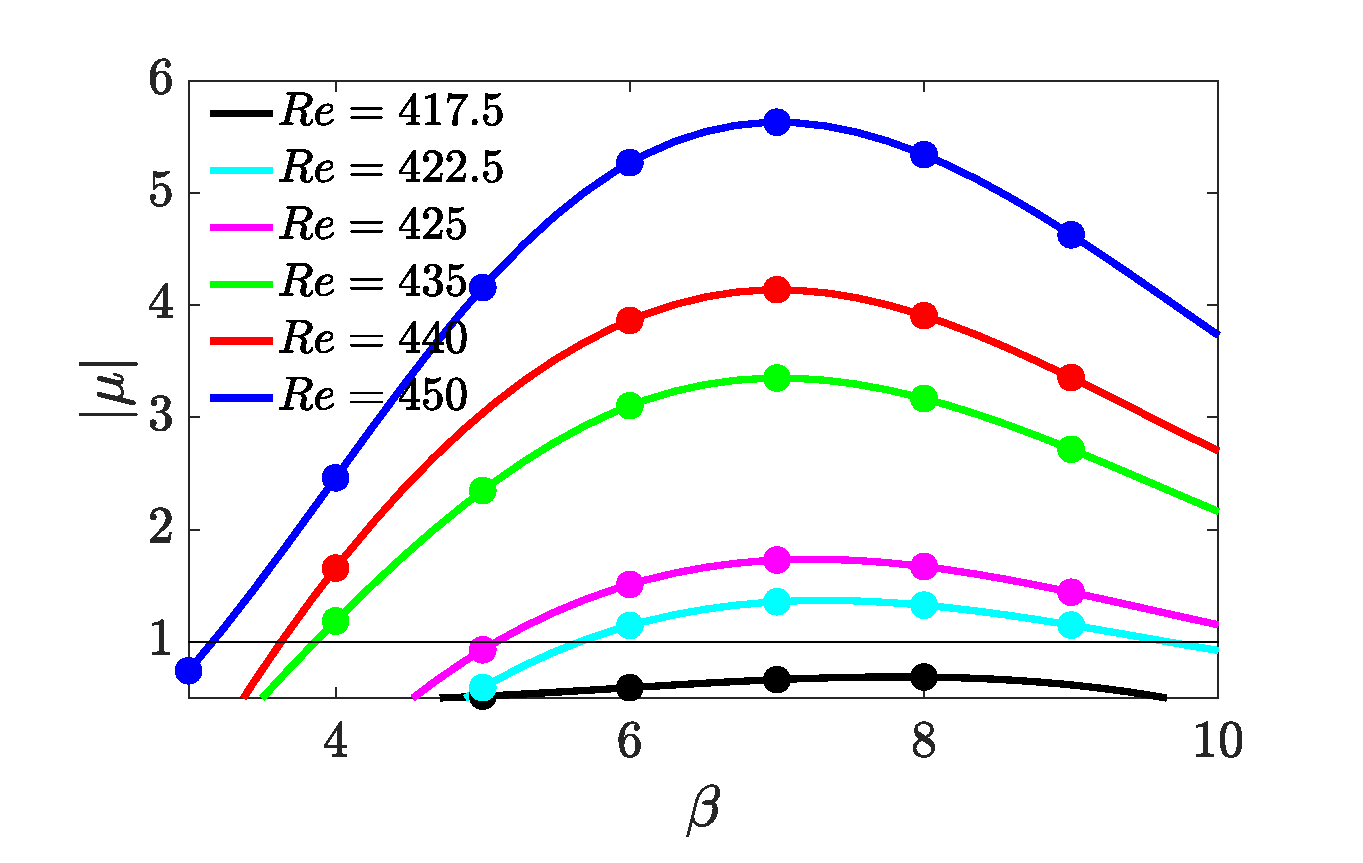
\includegraphics[width=0.49\textwidth]{./fig/AR4p5/multipliers_3D.eps}
\vspace{0.1cm}
\begin{tikzpicture}
\draw (-10,2) -- (8,2);
\end{tikzpicture}
\vspace{0.1cm}
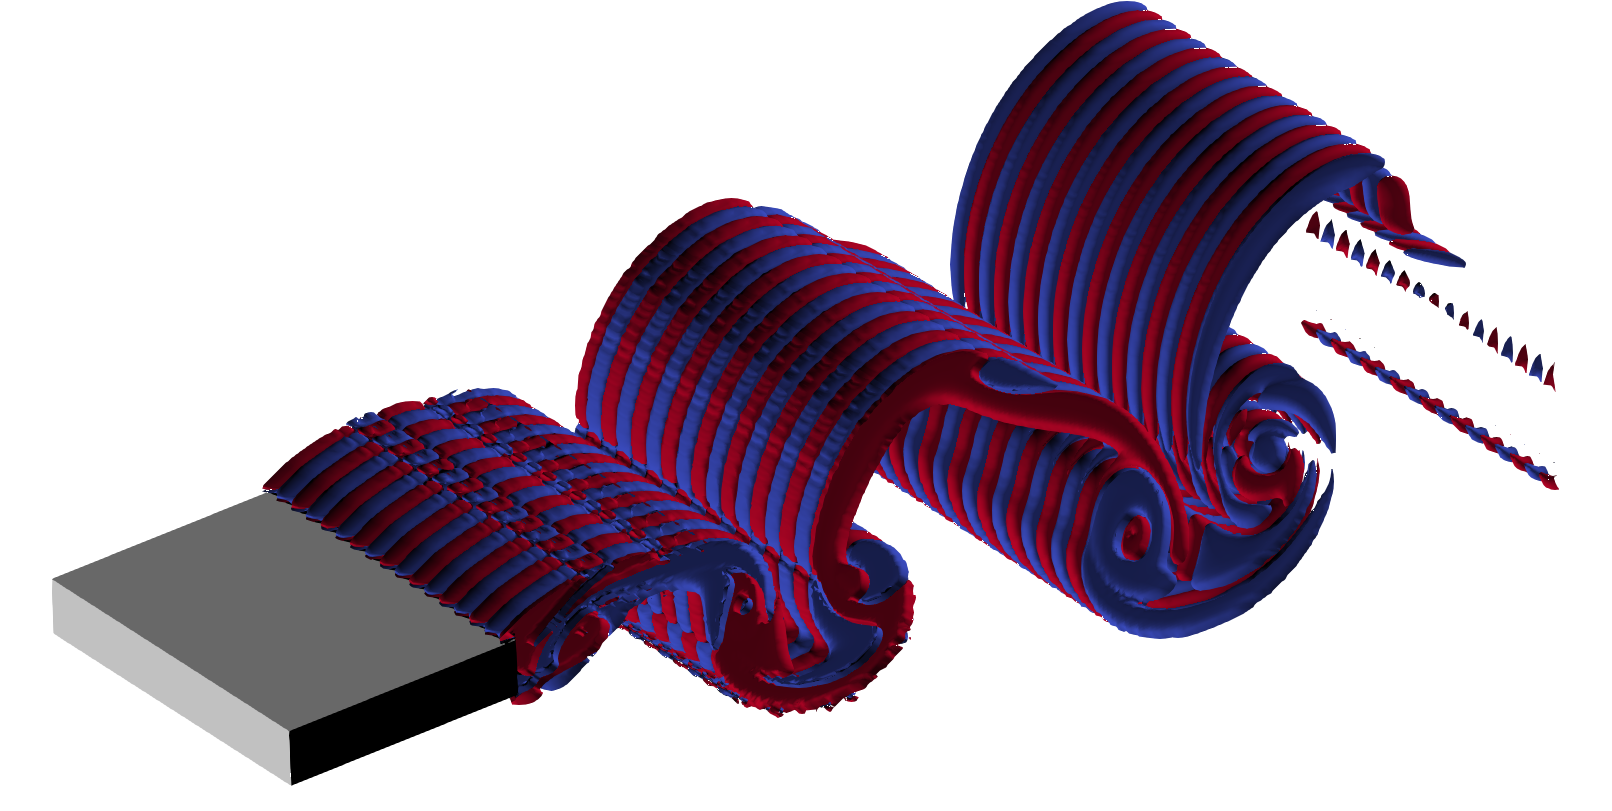
\includegraphics[trim={0 0 0 0},clip,width=0.49\textwidth]{./fig/AR4p5/Floqetmode_beta_8_Re450_AR4p5.png}
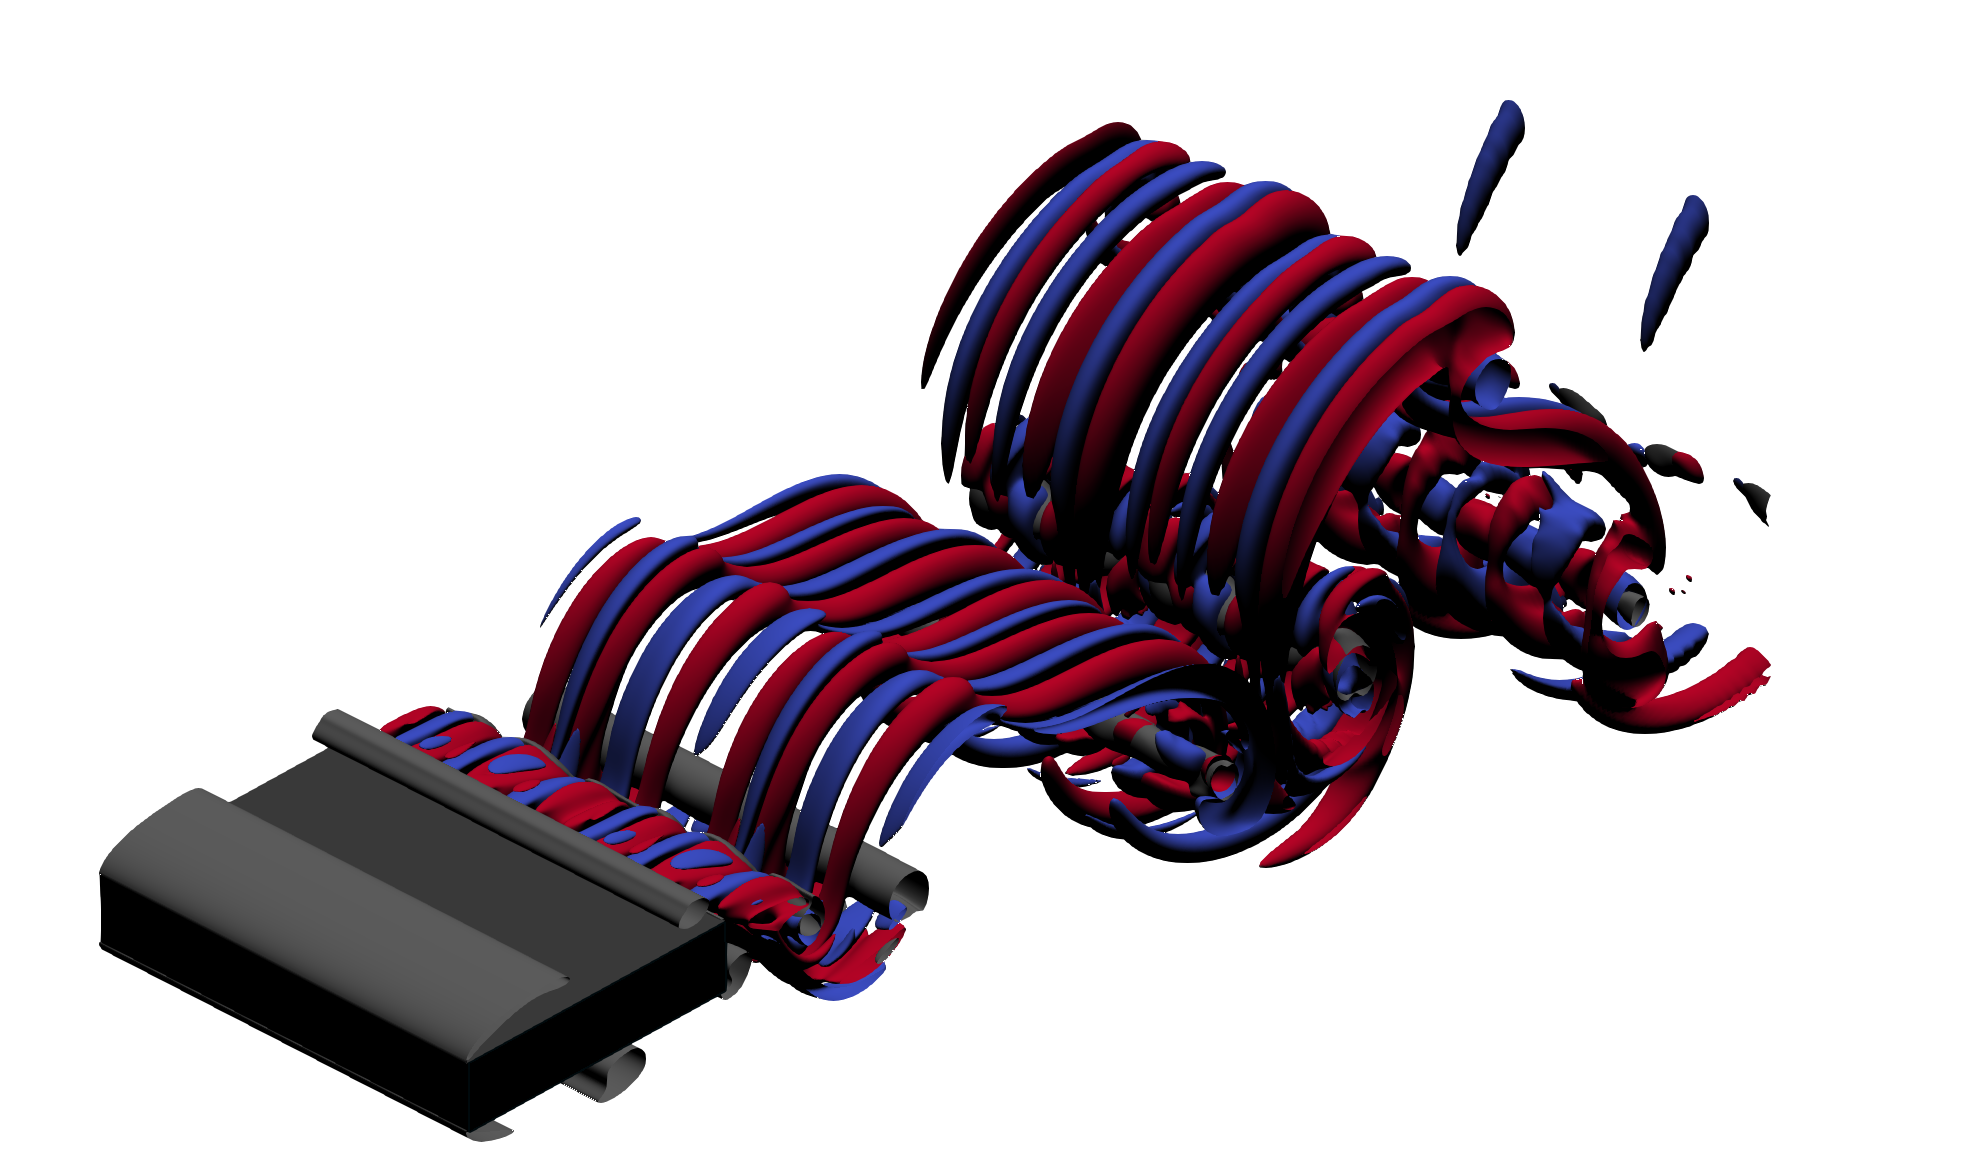
\includegraphics[width=0.49\textwidth]{./fig/AR4p5/lambda2_omegax-3D-Re450b.png}
\caption{Three-dimensional instability of the flow past a rectangular cylinder with $\AR=4.5$. The flow become unstable once the wake has bifurcated to a slanted configuration. The resulting limit cycle is (strongly) unstable to three-dimnsional perturbation of subharmonic nature (here the multipliers are real and negative); see top panel. Modes from the Floquet analysis for $\AR=4.5$. Bottom: Imaginary part of the streamwise vorticity for $\AR=4.5$, $Re=450$ and $\beta=8$ associated with the unstable subharmonic multiplier. Bottom right: DNS of the flow past the rectangular cylinder with $\AR=4.5$ at $Re=450$. Red/blue isosurfaces indicate $\omega_x = \pm 0.015$. Note that the wake is slanted and three-dimensional, as predicted by the Floquet stabilty analysis. The spanwise extent of the computational domain is $L_z=2\pi$.This means that the wavenumber associated with the three-dimensionality is $\beta \approx 6$, which is consistent with the most amplified wavenumber detected with the stability analysis.}
\label{fig:AR4p5_modes_Re430_beta0}
\end{figure}


%\begin{figure}
%\centering
%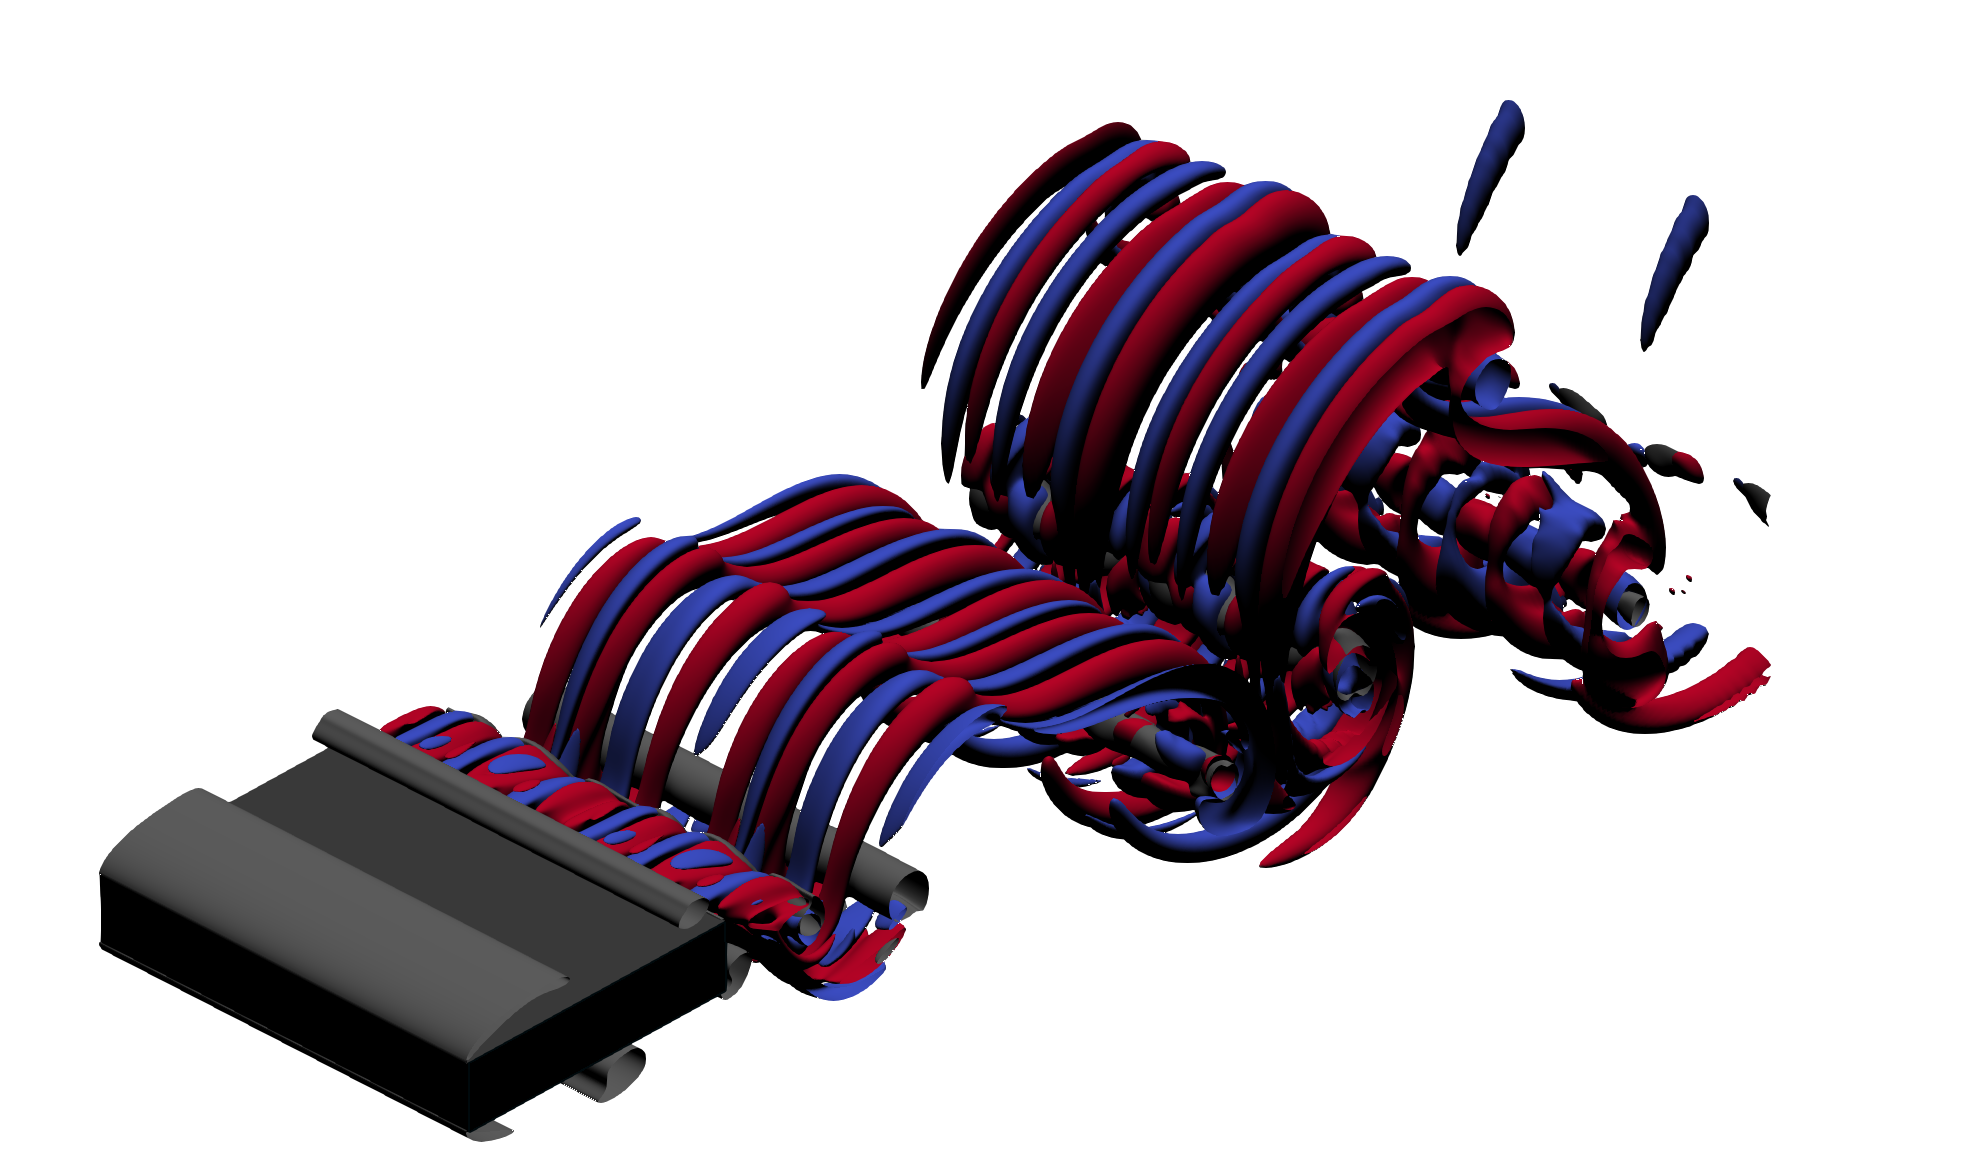
\includegraphics[width=0.7\textwidth]{./fig/AR4p5/lambda2_omegax-3D-Re450b.png}
%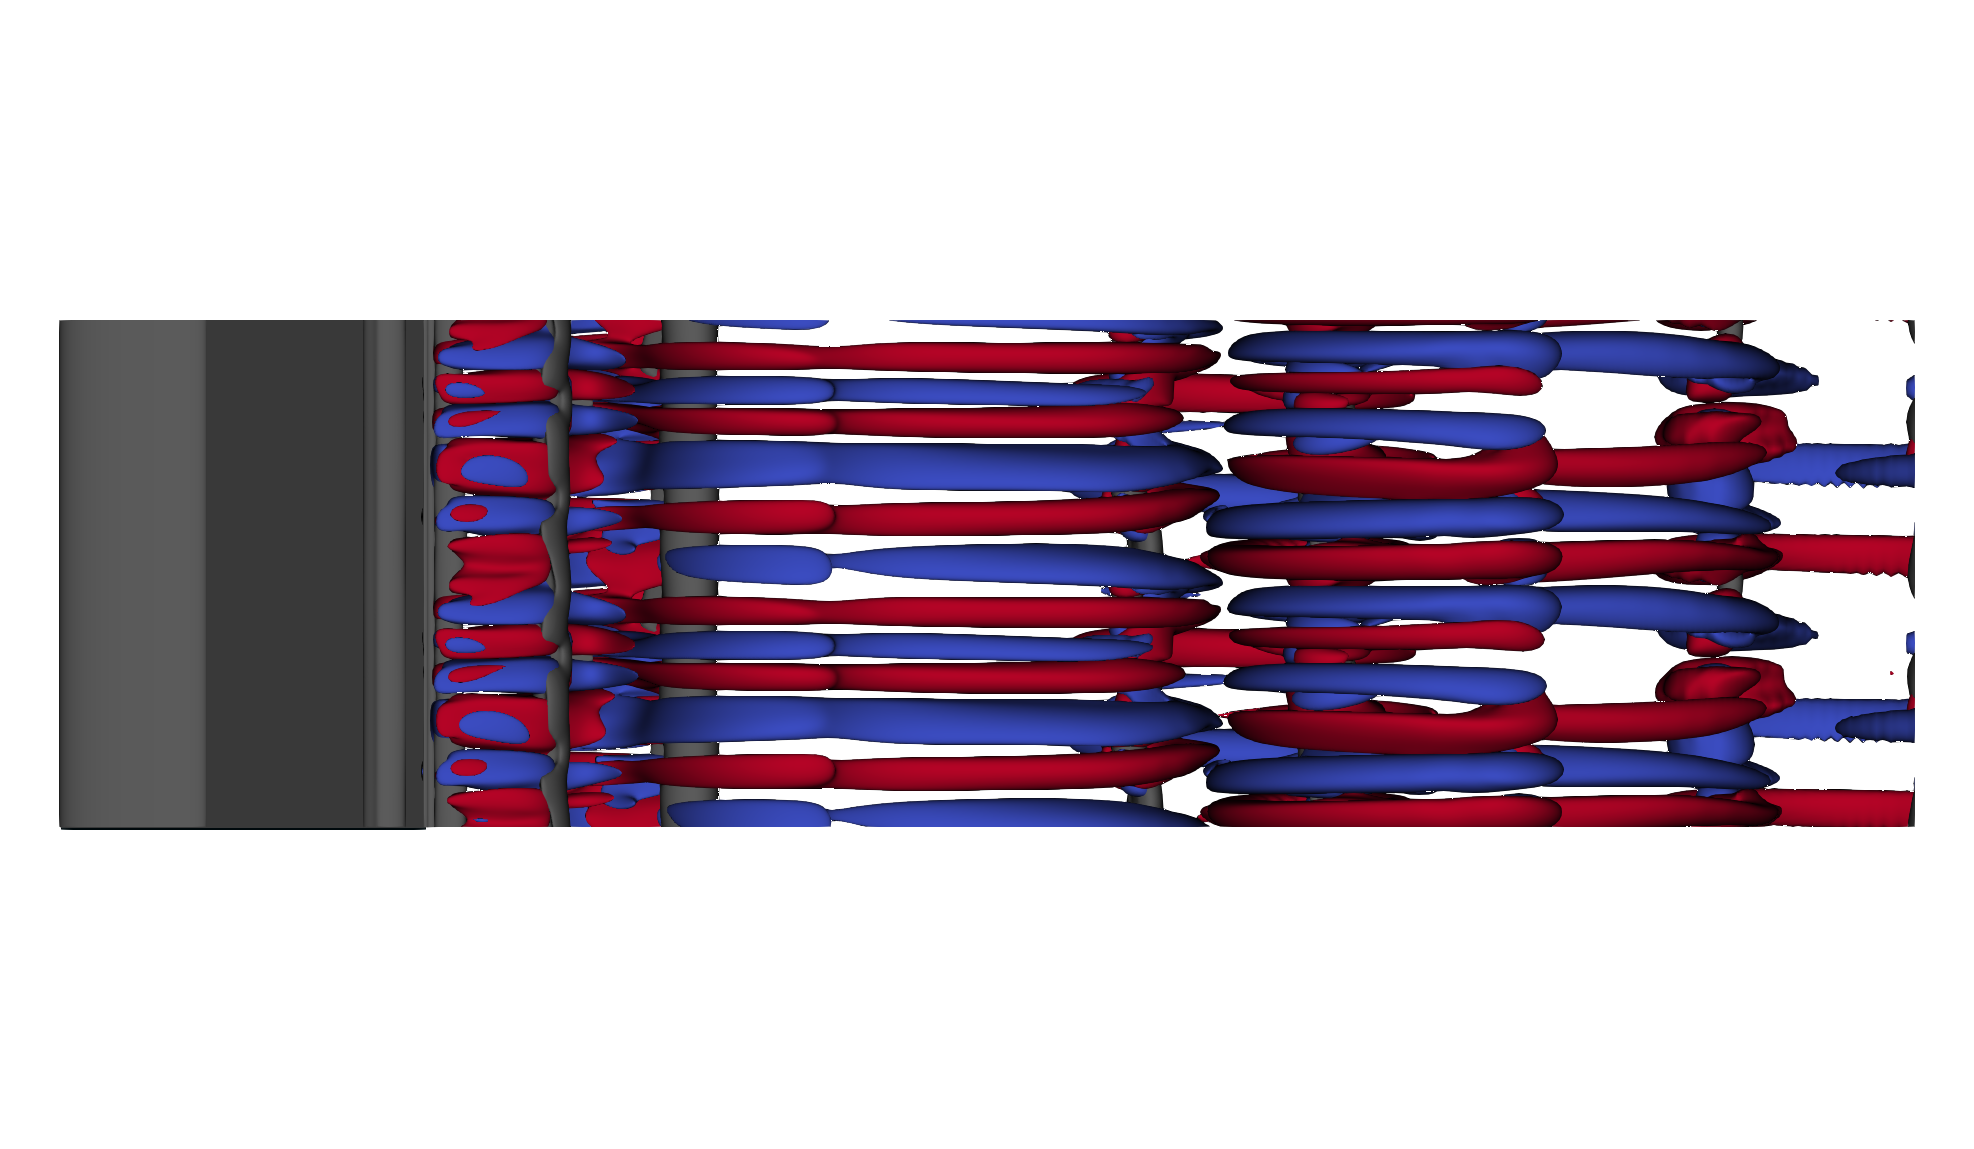
\includegraphics[trim=0 200 0 200,width=0.49\textwidth]{./fig/AR4p5/lambda2_omegax-xz-Re450b.png}
%\caption{DNS of the flow past the rectangular cylinder with $\AR=4.5$ at $Re=450$. Red/blue isosurfaces indicate $%\omega_x = \pm 0.015$. Note that the wake is slanted and three-dimensional, as predicted by the Floquet stabilty analysis. The spanwise extent of the computational domain is $L_z=2\pi$.This means that the wavenumber associated with the three-dimensionality is $\beta \approx 6$, which is consistent with the most amplified wavenumber detected with the stability analysis.}
%\label{fig:lambda2_omegax_AR45_Re450}
%\end{figure}
